\def\year{2019}\relax

\documentclass[letterpaper]{article}% DO NOT CHANGE THIS
\usepackage{aaai20}                 % DO NOT CHANGE THIS
\usepackage{times}                  % DO NOT CHANGE THIS
\usepackage{helvet}                 % DO NOT CHANGE THIS
\usepackage{courier}                % DO NOT CHANGE THIS
\usepackage[hyphens]{url}           % DO NOT CHANGE THIS
\usepackage{graphicx}               % DO NOT CHANGE THIS
\urlstyle{rm}                       % DO NOT CHANGE THIS
\def\UrlFont{\rm}                   % DO NOT CHANGE THIS
\usepackage{graphicx}               % DO NOT CHANGE THIS
\frenchspacing                      % DO NOT CHANGE THIS
\setlength{\pdfpagewidth}{8.5in}    % DO NOT CHANGE THIS
\setlength{\pdfpageheight}{11in}    % DO NOT CHANGE THIS

\nocopyright

\usepackage{epstopdf}
\usepackage{amssymb}
\usepackage{amsmath}
\usepackage{tikz}

\DeclareMathOperator*{\argmax}{arg\,max}

 \pdfinfo{
/Title (Multi-Fare Airline Ticket Dynamic Pricing Using Model-Free Reinforcement Learning)
/Author (Ross B. Alexander, Jonathan S. Ling)
/Keywords (dynamic pricing, multi-agent systems, reinforcement learning)
}

\setcounter{secnumdepth}{0}

\setlength\titlebox{2.5in} % If your paper contains an overfull \vbox too high warning at the beginning of the document, use this command to correct it. You may not alter the value below 2.5 in

\title{Multi-Segment Dynamic Pricing for Airline Tickets \\ Using Model-Free Reinforcement Learning}
\author{Ross B. Alexander \\ Department of Aeronautics and Astronautics \\ Stanford University \\ Stanford, CA 94305 \\ rbalexan@stanford.edu
\And Jonathan S. Ling \\ Department of Management Science and Engineering \\ Stanford University \\ Stanford, CA 94305 \\ jonling@stanford.edu}

\begin{document}

\maketitle

\begin{abstract}
    Dynamic pricing in the airline industry is the problem of optimally selling airline tickets over a finite horizon. Although optimal dynamic pricing can easily be achieved for a single customer segment, achieving optimal dynamic pricing for multiple competing customer segments is more difficult, as it sells from a common pooled inventory but does so at different price points. In this paper, we review common approaches taken to solve the single-segment dynamic pricing problem and formulate a multi-segment dynamic pricing problem using a factored multi-agent Markov decision process (MMDP) framework. We solve the multi-segment dynamic pricing problem using modern reinforcement learning (RL) approaches including Sarsa and Sarsa with eligibility traces and compare the performance of the approaches to various baseline policies.
\end{abstract}

\section{Introduction}

Dynamic pricing problems arise in many industries where goods and services are subject to a finite horizon. This finite horizon can be imposed both naturally or artificially, and often takes the form of perishability or expiration constraints of goods or services. In some cases, the inventory of goods or providers of services may also be finite. In attempting to maximize revenue, establishing a dynamic pricing policy can lead to increased revenue of a static pricing policy (Figure \ref{fig:static-dynamic-pricing}). A thorough survey of dynamic pricing reveals its pervasive presence in essentially all industries and as a result, the sheer variety of approaches taken to date to solve the dynamic pricing problems under the given constraints \cite{denBoer2015DynamicDirections}.

\begin{figure}[t]
    \centering
    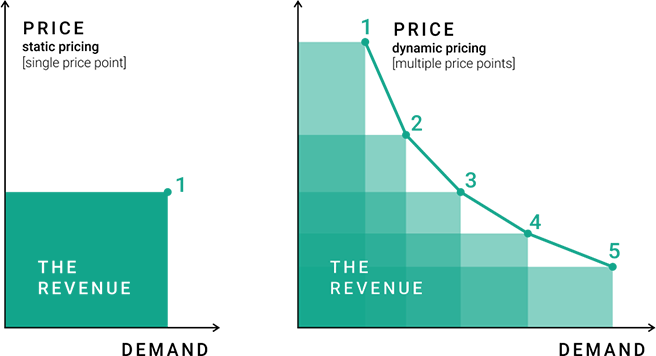
\includegraphics[width=0.99\linewidth]{final-paper/plots/static-dynamic-pricing.png}
    \caption{Maximization of revenue can be achieved using dynamic pricing policies instead of static pricing policies to exploit variation in demand. \cite{Competitoor2016Dynamic2016}}
    \label{fig:static-dynamic-pricing}
\end{figure}

In the airline industry, a natural dynamic pricing problem is evident -- an airline must maximize revenue for a finite set of tickets for a given flight before the flight departs, since sales cannot be made after the flight has departed. The airline must balance the certainty of selling all tickets, the maximization of revenue, and a stochastic demand. While most customers purchasing airline tickets likely know that the price of a given ticket fluctuates with time-to-departure, seasonality, trip type, etc., customers may be unaware that airlines typically offer a number of fare classes for various customer segments \textit{for the same seats on a single flight} (e.g. multiple fare classes for an economy ticket). For example, purchasing a one-way ticket, a return ticket spanning a weekend, or a return ticket spanning only business days will mean different costs to the customer for the same leg of the journey, despite being for the same seat. The International Air Transport Association (IATA) has standardized a system of 26 different fare classes (formally called \textit{Reservation Booking Designators}) that airlines use to characterize these different customer segments, which thus gives rise to 26 possible price points \cite{Touraine2018DynamicPaper}. As a result, a critical but often unseen dynamic pricing problem naturally arises in the airline industry for maximizing revenue over the different fare classes for a single flight.

Decision theory provides a foundation for formulating these types dynamic pricing problems, and dynamic programming and reinforcement learning provide methods for solving these problems to generate an optimal or approximately optimal pricing policy. More detail is given in the Proposed Approach section, and a survey of decision-theoretic approaches for airline ticket dynamic pricing problems is given in \citeauthor{Abdella2019} (\citeyear{Abdella2019}).

Based on a review given by \citeauthor{Rana2014Real-timeLearning} in \citeyear{Rana2014Real-timeLearning}, in the 2000's, most dynamic pricing problems were solved using model-based reinforcement learning methods that explicitly described the interaction of demand and pricing. While these model-based approaches were widely popular and quite accurate, misrepresentation of the model led to reduced performance of these dynamic pricing policies. Model-free approaches are a relatively new area of research, and are proving to be more relevant given the explosion of big data applications, unknown and complex model structures, and high-uncertainty situations. 

Here, we provide a brief survey of model-free approaches to the dynamic pricing problem in the literature. \citeauthor{Carvalho2003DynamicLearning} (\citeyear{Carvalho2003DynamicLearning}) have studied parametric forms of the customer arrival distribution, and used reinforcement learning to estimate the parameters to predict demand and compute optimal dynamic policies, partially bridging the gap between model-based and model-free approaches. \citeauthor{Rana2014Real-timeLearning} (\citeyear{Rana2014Real-timeLearning}) have used reinforcement learning and Q-learning to compute optimal pricing policies under incomplete information and non-stationary demand. We extend this by considering multiple customer segments. \citeauthor{Raju2006LearningSegmentation} (\citeyear{Raju2006LearningSegmentation}) have used Q-learning to dynamically price products with customer segmentation, but their segments are specially characterized and do not allow for generalizations to more segments, which we study.

This paper adds to the dynamic pricing reinforcement learning literature by considering how to price for multiple customer segments from a single pooled inventory source.

\section{Proposed Approach}

\subsection{MMDP Background}

In the general hierarchy of decision-theoretic approaches for solving multi-agent sequential decision-making under uncertainty problems (Figure \ref{fig:multiagent-framework-hierarchy}), the most general framework is the partially-observable stochastic game (POSG) where each agent maintains its own individually partially-observable state space, action space, observation space, and reward model \cite{Hansen2004DynamicGames}. Decentralized partially-observable Markov decision processes (DEC-POMDPs) are a subclass of POSGs that have a single reward model rather than a reward model for each agent, though the agents' objectives may still be competing. Decentralized Markov decision processes (DEC-MDPs) are a subclass of DEC-POMDPs characterized by joint full-observability of the joint state, and multi-agent Markov decision processes (MMDPs) are a subclass of DEC-MDPs characterized by individual full-observability of the joint state. A detailed overview of DEC-POMDPs and their subclasses is given in \citeauthor{doi:10.1002/9781118557426.ch9} \citeyear{doi:10.1002/9781118557426.ch9}.

\begin{figure}[b]
    \centering
    \tikzset{every picture/.style={line width=0.75pt}} %set default line width to 0.75pt        
    \begin{tikzpicture}[x=0.75pt,y=0.75pt,yscale=-0.95,xscale=0.77]
    %uncomment if require: \path (0,300); %set diagram left start at 0, and has height of 300
    
    %Shape: Ellipse [id:dp4251694647784602] 
    \draw   (206,143.29) .. controls (206,125.22) and (255.02,110.57) .. (315.5,110.57) .. controls (375.98,110.57) and (425,125.22) .. (425,143.29) .. controls (425,161.35) and (375.98,176) .. (315.5,176) .. controls (255.02,176) and (206,161.35) .. (206,143.29) -- cycle ;
    %Shape: Ellipse [id:dp06475026590390243] 
    \draw   (46,143.29) .. controls (46,125.22) and (95.02,110.57) .. (155.5,110.57) .. controls (215.98,110.57) and (265,125.22) .. (265,143.29) .. controls (265,161.35) and (215.98,176) .. (155.5,176) .. controls (95.02,176) and (46,161.35) .. (46,143.29) -- cycle ;
    %Shape: Ellipse [id:dp8014248709484794] 
    \draw   (207,143.29) .. controls (207,128.1) and (236.55,115.79) .. (273,115.79) .. controls (309.45,115.79) and (339,128.1) .. (339,143.29) .. controls (339,158.47) and (309.45,170.79) .. (273,170.79) .. controls (236.55,170.79) and (207,158.47) .. (207,143.29) -- cycle ;
    %Shape: Ellipse [id:dp27296915659951937] 
    \draw   (38,143) .. controls (38,109.31) and (126.42,82) .. (235.5,82) .. controls (344.58,82) and (433,109.31) .. (433,143) .. controls (433,176.69) and (344.58,204) .. (235.5,204) .. controls (126.42,204) and (38,176.69) .. (38,143) -- cycle ;
    %Shape: Ellipse [id:dp17544716770223856] 
    \draw   (29.5,142) .. controls (29.5,91.19) and (121.73,50) .. (235.5,50) .. controls (349.27,50) and (441.5,91.19) .. (441.5,142) .. controls (441.5,192.81) and (349.27,234) .. (235.5,234) .. controls (121.73,234) and (29.5,192.81) .. (29.5,142) -- cycle ;
    
    % Text Node
    \draw (236.5,143.29) node  [align=left] {MDP};
    % Text Node
    \draw (295.5,143.29) node  [align=left] {MMDP};
    % Text Node
    \draw (381.5,143.29) node  [align=left] {DEC-MDP};
    % Text Node
    \draw (155.5,143.29) node  [align=left] {POMDP};
    % Text Node
    \draw (235.5,99) node  [align=left] {DEC-POMDP};
    % Text Node
    \draw (235.5,68) node  [align=left] {POSG};
    
    
    \end{tikzpicture}
    \caption{Hierarchy of decision-theoretic approaches for multi-agent sequential decision-making under uncertainty.}
    \label{fig:multiagent-framework-hierarchy}
\end{figure}

\begin{figure}[t]
    \centering
    \tikzset{every picture/.style={line width=0.75pt}} %set default line width to 0.75pt 
    \begin{tikzpicture}[x=0.75pt,y=0.75pt,yscale=-0.9,xscale=0.9]
%uncomment if require: \path (0,450); %set diagram left start at 0, and has height of 450

%Shape: Circle [id:dp7971837618192504] 
\draw   (88,253) .. controls (88,239.19) and (99.19,228) .. (113,228) .. controls (126.81,228) and (138,239.19) .. (138,253) .. controls (138,266.81) and (126.81,278) .. (113,278) .. controls (99.19,278) and (88,266.81) .. (88,253) -- cycle ;
%Shape: Circle [id:dp4245933526012209] 
\draw   (227,253) .. controls (227,239.19) and (238.19,228) .. (252,228) .. controls (265.81,228) and (277,239.19) .. (277,253) .. controls (277,266.81) and (265.81,278) .. (252,278) .. controls (238.19,278) and (227,266.81) .. (227,253) -- cycle ;
%Straight Lines [id:da27108952217182103] 
\draw    (138,253) -- (224,253) ;
\draw [shift={(227,253)}, rotate = 180] [fill={rgb, 255:red, 0; green, 0; blue, 0 }  ][line width=0.08]  [draw opacity=0] (8.93,-4.29) -- (0,0) -- (8.93,4.29) -- cycle    ;

%Shape: Square [id:dp2484773301173374] 
\draw   (92.5,20) -- (133.5,20) -- (133.5,61) -- (92.5,61) -- cycle ;
%Shape: Diamond [id:dp6458027862228564] 
\draw   (113,118.25) -- (138.75,144) -- (113,169.75) -- (87.25,144) -- cycle ;

%Straight Lines [id:da8485112219933894] 
\draw    (112.5,61) -- (225.46,250.42) ;
\draw [shift={(227,253)}, rotate = 239.19] [fill={rgb, 255:red, 0; green, 0; blue, 0 }  ][line width=0.08]  [draw opacity=0] (8.93,-4.29) -- (0,0) -- (8.93,4.29) -- cycle    ;

%Straight Lines [id:da8093839051067403] 
\draw    (113,228) -- (113,172.75) ;
\draw [shift={(113,169.75)}, rotate = 450] [fill={rgb, 255:red, 0; green, 0; blue, 0 }  ][line width=0.08]  [draw opacity=0] (8.93,-4.29) -- (0,0) -- (8.93,4.29) -- cycle    ;

%Straight Lines [id:da553758533588754] 
\draw    (112.5,61) -- (112.97,115.25) ;
\draw [shift={(113,118.25)}, rotate = 269.5] [fill={rgb, 255:red, 0; green, 0; blue, 0 }  ][line width=0.08]  [draw opacity=0] (8.93,-4.29) -- (0,0) -- (8.93,4.29) -- cycle    ;

%Rounded Rect [id:dp9390891470163364] 
\draw   (50.5,18) .. controls (50.5,11.92) and (55.42,7) .. (61.5,7) -- (162.5,7) .. controls (168.58,7) and (173.5,11.92) .. (173.5,18) -- (173.5,78.63) .. controls (173.5,84.7) and (168.58,89.63) .. (162.5,89.63) -- (61.5,89.63) .. controls (55.42,89.63) and (50.5,84.7) .. (50.5,78.63) -- cycle ;
%Shape: Circle [id:dp7810602827185217] 
\draw   (88,356) .. controls (88,342.19) and (99.19,331) .. (113,331) .. controls (126.81,331) and (138,342.19) .. (138,356) .. controls (138,369.81) and (126.81,381) .. (113,381) .. controls (99.19,381) and (88,369.81) .. (88,356) -- cycle ;
%Shape: Circle [id:dp6780539984791033] 
\draw   (227,356) .. controls (227,342.19) and (238.19,331) .. (252,331) .. controls (265.81,331) and (277,342.19) .. (277,356) .. controls (277,369.81) and (265.81,381) .. (252,381) .. controls (238.19,381) and (227,369.81) .. (227,356) -- cycle ;
%Rounded Rect [id:dp26692211648926156] 
\draw   (212.5,334) .. controls (212.5,326.82) and (218.32,321) .. (225.5,321) -- (281.5,321) .. controls (288.68,321) and (294.5,326.82) .. (294.5,334) -- (294.5,390.63) .. controls (294.5,397.8) and (288.68,403.63) .. (281.5,403.63) -- (225.5,403.63) .. controls (218.32,403.63) and (212.5,397.8) .. (212.5,390.63) -- cycle ;
%Straight Lines [id:da5535478530681583] 
\draw    (138,253) -- (225.04,353.73) ;
\draw [shift={(227,356)}, rotate = 229.17000000000002] [fill={rgb, 255:red, 0; green, 0; blue, 0 }  ][line width=0.08]  [draw opacity=0] (8.93,-4.29) -- (0,0) -- (8.93,4.29) -- cycle    ;

%Straight Lines [id:da45351505035954487] 
\draw    (138,356) -- (224,356) ;
\draw [shift={(227,356)}, rotate = 180] [fill={rgb, 255:red, 0; green, 0; blue, 0 }  ][line width=0.08]  [draw opacity=0] (8.93,-4.29) -- (0,0) -- (8.93,4.29) -- cycle    ;

%Straight Lines [id:da30858363643947473] 
\draw    (138,356) -- (225.04,255.27) ;
\draw [shift={(227,253)}, rotate = 490.83] [fill={rgb, 255:red, 0; green, 0; blue, 0 }  ][line width=0.08]  [draw opacity=0] (8.93,-4.29) -- (0,0) -- (8.93,4.29) -- cycle    ;

%Straight Lines [id:da7765491376645027] 
\draw    (112.5,61) -- (225.91,353.2) ;
\draw [shift={(227,356)}, rotate = 248.79000000000002] [fill={rgb, 255:red, 0; green, 0; blue, 0 }  ][line width=0.08]  [draw opacity=0] (8.93,-4.29) -- (0,0) -- (8.93,4.29) -- cycle    ;

%Rounded Rect [id:dp33428251319510194] 
\draw   (70.5,335) .. controls (70.5,327.82) and (76.32,322) .. (83.5,322) -- (139.5,322) .. controls (146.68,322) and (152.5,327.82) .. (152.5,335) -- (152.5,391.63) .. controls (152.5,398.8) and (146.68,404.63) .. (139.5,404.63) -- (83.5,404.63) .. controls (76.32,404.63) and (70.5,398.8) .. (70.5,391.63) -- cycle ;
%Curve Lines [id:da2562950314163758] 
\draw    (113,331) .. controls (111.39,295.52) and (155.08,288.96) .. (155.5,255) .. controls (155.91,221.55) and (148.88,207.18) .. (114.59,171.4) ;
\draw [shift={(113,169.75)}, rotate = 406.05] [fill={rgb, 255:red, 0; green, 0; blue, 0 }  ][line width=0.08]  [draw opacity=0] (8.93,-4.29) -- (0,0) -- (8.93,4.29) -- cycle    ;


% Text Node
\draw (252,253) node   {$s^{t+1}_{0}$};
% Text Node
\draw (113,144) node   {$r^{t}$};
% Text Node
\draw (113,253) node   {$s^{t}_{0}$};
% Text Node
\draw (82,79) node [scale=0.7]  {$i=1,...,n$};
% Text Node
\draw (113,40.5) node [scale=1]  {$a^{t}_{i}$};
% Text Node
\draw (252,356) node   {$s^{t+1}_{i}$};
% Text Node
\draw (113,356) node   {$s^{t}_{i}$};
% Text Node
\draw (244,392) node [scale=0.7]  {$i=1,...,n$};
% Text Node
\draw (102,393) node [scale=0.7]  {$i=1,...,n$};


\end{tikzpicture}
    \caption{Structure of the factored multi-agent Markov decision process (MMDP) as a dynamic decision network.}
    \label{fig:mmdp-ddn-diagram}
\end{figure}

An MMDP \cite{Boutilier1999SequentialSystems} is defined by the 5-tuple $\langle n, \mathcal{S}, \mathcal{A}, T, R \rangle$ where $n$ is the number of agents ($i \in \{1, ..., n\}$), $\mathcal{S}$ is the joint state space, $\mathcal{A}$ is the joint action space, $T$ is the transition model, and $R$ is the reward model. 

In a factored MMDP, depicted in Figure \ref{fig:mmdp-ddn-diagram}, the joint state space can be factored into a representation composed of the environment state space $\mathcal{S}_0$ and the local state space $\mathcal{S}_i$ for agent $i$ such that the joint state space $\mathcal{S} = \mathcal{S}_0 \times \mathcal{S}_1 \times ... \times \mathcal{S}_n$. The joint state $s$, which is jointly fully-observable, is thus the specific state given by the environmental state $s_0$ and sub-state $s_i$ of all $n$ agents ($s = \langle s_0, s_1, ..., s_n \rangle$).  The joint action space can be represented similarly using the action space $\mathcal{A}_i$ for agent $i$ such that the joint action space $\mathcal{A} = \mathcal{A}_1 \times ... \times \mathcal{A}_n$. The joint action $a$ is given by the actions $a_i$ of all $n$ agents ($a = \langle a_1, ..., a_n \rangle$). The transition model gives the probability $T(s, a, s')$ of transitioning to joint state $s'$ from the joint state $s$ after executing the joint action $a$. A general factored MMDP does not necessarily have transition independence; in general, $T \neq T(s_i, a, s_i')$. Additionally, the reward model $R(s, a, s')$ is the reward received for transitioning to joint state $s'$ from the joint state $s$ after executing the joint action $a$. 

Note that MMDPs contain all Markov decision processes (MDPs), since all MDPs are degenerate 1-agent MMDPs (i.e. $\langle \mathcal{S}, \mathcal{A}, T, R \rangle \triangleq \langle 1, \mathcal{S}, \mathcal{A}, T, R \rangle$). The solution to an MMDP is given by a joint policy $\pi = \langle \pi_1, ..., \pi_n \rangle$.  The complexity of solving an MMDP is known to be P-complete \cite{Papadimitriou1987TheProcesses}.

\subsection{Dynamic Pricing Problem}

The multi-fare dynamic pricing problem is the problem of maximizing revenue for a given flight that has some finite number of seats with underlying non-stationary demand for these seats across multiple categories, and a flight departure date that induces a finite horizon. Since we can utilize customer details provided in a trip query (e.g., one-way/return, length of trip, etc.), we can develop multiple fare classes (price classes) to exploit latent differences between such demand categories and maximize revenue. Thus, agency in our dynamic pricing problem is a representation of each fare class' independent pricing and sale of tickets. We consider the case where the seats are identical and fungible (e.g. all in economy), and thus the number of tickets available is from a common inventory pool. 

It should also be noted that although the customer dynamics are stationary -- customers arriving at each time step are defined by distributions that do not change with time -- the customer arrival dynamics are non-stationary -- fewer customers arrive as the departure date approaches -- so the aggregate demand dynamics are non-stationary.

For the dynamic pricing problem, we use a discretization of the joint state and action spaces to generate the joint state and action sets, respectively. Environmental state variables include the number of tickets available and a discretized time. We characterize agents by the different fare classes. Each agent's sub-state variable is the number of tickets sold for their fare class, and the agent's action is a ticket price for their fare class. The transition model is formulated as a generative model based on customer dynamics to compute the new joint state after taking the joint action from the previous joint state, since the exact transition probabilities are difficult to represent explicitly. The reward model, describing the total revenue, is exactly known, and is easily computed as the sumproduct of ticket prices and quantities sold across all fare classes.

\subsubsection{Joint State Set} 

In our dynamic pricing problem, the environment state $s_0$ is defined by the tuple $(v, t) \in \{0, ..., V\} \times \{0, ..., T\}$, representing the number of available tickets (or vacant seats) $v$ given the number of initially available tickets $V$, and the time $t$ given the finite horizon $T$. The sub-state $s_i$ for agent $i$ is defined as the number of tickets sold $u \in \{0, ..., V\}$ in the previous time step.

\subsubsection{Joint Action Set}

The action $a_i$ for agent $i$ is defined as the ticket price $a_i \in \{ \underline{p_i}, \underline{p_i}+\tilde{p_i}, \underline{p_i}+2\tilde{p_i}, ..., \overline{p_i} \}$ given the agent's lower and upper pricing bounds, $\underline{p_i}$ and $\overline{p_i}$, and some spacing constant $\tilde{p_i}$, such that the cardinality of the agent's action set is fixed (e.g. $|\mathcal{A}_i| = 10$).

\subsubsection{Transition Model}

The transition model that maps the current joint state $s$, the joint action $a$, and next joint state $s'$ to a probability $T:\mathcal{S} \times \mathcal{A} \times \mathcal{S} \rightarrow \mathbb{R}$ with probability constraints $T(s,a,s')\geq 0$ and $\sum_{s'} T(s,a,s') = 1 \, \forall \, s,a$ cannot be explicitly represented for our dynamic pricing problem without knowing the customer dynamics. However, the transition from $s$ to $s'$ after executing $a$ can be formulated. 

Since the dynamic pricing MMDP employs a factored state, we can describe the transition in terms of the environment state transition $s_0 \rightarrow s_0'$ and the sub-state transition for agent $i$, $s_i \rightarrow s_i'$. 

For agent $i$, we define a set of customers seeking tickets $C_i$ (initially empty). At each time step, we have $n_i$ new customers arriving according to a Poisson distribution with a linearly time-varying parameter governed by the fare class parameters $\alpha_i$ and $\beta_i$, such that $n_i \sim \textnormal{Pois}(n \mid \alpha_i t+\beta_i)$. The $j$th new customer $c_{i,j} \, \forall \, j \in \{1, ..., n_i\}$ has some willingness-to-pay (WTP) price threshold $w_j \sim \mathcal{N}(w_j \mid \mu_i, \sigma_i)$ and some willingness-to-pay (WTP) flexibility $k_j \sim \mathcal{U}(k_j \mid a_i, b_i)$. The customer purchase dynamics follow the given cases, with $b_j = 1$ if the customer purchases the ticket and $b_j = 0$ if the customer does not purchase the ticket:
\begin{equation}
    \begin{cases}
      b_j \sim \textnormal{Bernoulli}(b_j \mid 2\cdot(1-\Phi(a_i))) & \text{if $a_i > w_j$}\\
      b_j = 1 & \text{if $a_i \leq w_j$}
    \end{cases}  \nonumber     
\end{equation}
where $\Phi = \textnormal{CDF}(\textnormal{Logistic}(a_i \mid w_j, k_j))$. If the customer $c_{i,j}$ purchases a ticket, they are removed from the agent's set of customers $C_i \leftarrow C_i \setminus \{c_{i,j}\}$.

Then the environment state $s_0 = (v, t)$ is updated by subtracting the number of tickets sold by all agents in the previous time step and incrementing $t$ such that $s_0'=(v-\sum_i s_i', t+1)$.

\subsubsection{Reward Model}

The joint reward is the revenue $r$ received from the sales of tickets at their respective prices, which enables an explicit representation of the reward function using agent-wise additive decomposition so that $r = \sum_{i=1}^n a_i s_i'$ or, using vector representations of the joint action $\textbf{a}$ and new joint state excluding the new environment state $\mathbf{s}_{\setminus 0}'$, $r = \textbf{a}^T\textbf{s}_{\setminus 0}'$. 

\subsection{Model-Free Reinforcement Learning}

Although the dynamic pricing MMDP is defined by the tuple $\langle 1, \mathcal{S}, \mathcal{A}, T, R \rangle$, the transition model cannot be explicitly represented. As a result, a model-free method for determining an optimal or approximately optimal policy must be used. 

Q-learning is a model-free reinforcement learning approach that focuses on learning a state-action value function $Q$ that maps the state and action to the expected future reward $Q: \mathcal{S} \times \mathcal{A} \rightarrow \mathbb{R}$. The corresponding policy $\pi: \mathcal{S} \rightarrow \mathcal{A}$ for the given state-action value function is given by $\pi(s) = \argmax_a Q(s,a) \, \forall \, s$. Most Q-learning methods utilize two parameters for learning, namely $\alpha$, the learning rate, and $\gamma$, the discount factor. Q-learning employs incremental estimation of Bellman equation for dynamic programming such that in the limit, the equality is satisfied. The Bellman equation for Q-learning is:
\begin{align*}
Q(s,a) &= R(s,a) + \gamma \sum_{s'} T(s, a, s')U(s') \\ 
Q(s,a) &= R(s,a) + \gamma \sum_{s'} T(s, a, s') \max_{a'}Q(s', a') 
\end{align*}

\subsubsection{Q-Learning}

It is straightforward to prove that the temporal difference (TD) update for Q-learning is:
$$ Q(s,a) \leftarrow Q(s,a) + \alpha \left( r + \gamma \max_{a'} Q(s', a') - Q(s,a) \right)$$
implying a complexity per state-action update of $\mathcal{O}(|\mathcal{A}|)$.

\subsubsection{Sarsa}

Another prominent Q-learning algorithm is the Sarsa algorithm, which was first proposed by \citeauthor{Rummery1994OnlineSystems} in \citeyear{Rummery1994OnlineSystems} and derives its name from requiring the tuple $(s,a,r,s',a')$ to compute the update. Sarsa uses the next state $s'$ and the next action $a'$ to remove the the maximization over all actions in the Q-learning TD update. From this, it is straightforward to prove that the TD update for Sarsa is:
$$ Q(s,a) \leftarrow Q(s,a) + \alpha \left( r + \gamma Q(s', a') - Q(s,a) \right)$$ 
implying a complexity per state-action update of $\mathcal{O}(1)$.

\subsubsection{Eligibility Traces} 

Both Q-learning and Sarsa can be modified with eligibility traces (often called Q($\lambda$) and Sarsa($\lambda$)). Eligibility traces employ an additional exponential decay parameter $\lambda$ to recursively assign partial credit proportional to $\lambda^t$ backwards along the state-action history (the eligible trace), which can help speed learning in both complex and sparse-reward environments.

\section{Experimental Setup}

We performed two sets of experiments, namely, determining and optimal policy for a single fare class (Class 1) and for two fare classes (Class 1 \& Class 2). The class parameters were constant throughout the experiments and are listed in Table \ref{tab:fare-class-params}.

\begin{table}[h!]
 \caption{Fare Class Parameters}
    \vspace{10 pt}
    \label{tab:fare-class-params}
    \centering
    \begin{tabular}{l|cc}
        \hline \hline
        \textbf{Parameter -- Description} & \textbf{Class 1} & \textbf{Class 2}  \\ \hline
        $\alpha$ -- cust. arr. rate slope    & -1 & -1 \\
        $\beta$ -- cust. arr. rate intercept & 30 & 20 \\
        $\mu$ -- WTP threshold mean          & 700 & 300  \\
        $\sigma$ -- WTP threshold SD         & 100 & 50 \\
        $a$ -- WTP flexibility LB            & 20 & 10 \\ 
        $b$ -- WTP flexibility UB            & 20.1 & 10.1  \\
        $\underline{p}$ -- price LB          & 550 & 225   \\
        $\overline{p}$ -- price UB           & 850 & 375  \\
        $\tilde{p}$ -- price interval        & 75 & 37.5  \\
        \hline \hline
    \end{tabular}
\end{table}

For each problem, both Sarsa and Sarsa($\lambda$) were performed to compute optimal policies and were compared against optimal policies that were allowed to learn the state-action value function given an exploration policy. These exploration policies includd a static low policy (offering the lowest price at all times for all fare classes), a static high policy (offering the highest price at all times for all fare classes), and a random policy. The parameters governing the two problems are given in Table \ref{tab:fare-class-solver-params}. The problem is undiscounted $\gamma = 1$ since the horizon is finite.

\vspace{40 pt}

\begin{table}[h!]
 \caption{Solver Parameters}
    \vspace{10 pt}
    \label{tab:fare-class-solver-params}
    \centering
    \begin{tabular}{l|cc}
        \hline \hline
        \textbf{Parameter} & \textbf{One Class} &\textbf{Two Classes} \\ \hline
        Time horizon             & 20 & 20 \\
        Number of tickets avail. & 300 & 500 \\
        Learning rate            & 0.1 & 0.2 \\
        Discount factor          & 1 & 1 \\
        Eligibility parameter    & 0.9 & 0.9 \\
        Training episodes        & 250,000 & 50,000 \\
        Exploration strategy     & $\epsilon$-greedy & $\epsilon$-greedy\\
        $\epsilon$               & 0.2 & 0.2 \\
        \hline \hline
    \end{tabular}
\end{table}

\section{Results}

The average rewards for executing the baseline optimal policies and the optimal policies for each of the fare classes is tabulated in Table \ref{tab:fare-class-rewards}.

\begin{table}[h!]
 \caption{Fare Class Optimal Policy Average Rewards}
    \vspace{10 pt}
    \label{tab:fare-class-rewards}
    \centering
    \begin{tabular}{l|cc}
        \hline \hline
        \textbf{Policy} & \textbf{One Class} & \textbf{Two Classes} \\ \hline
        Static low       & 165,000 & 217,684 \\
        Static high      & 75,424 & 92,776 \\
        Random           & 188,729 & 250,003 \\
        Sarsa            & 190,758 & 239,400 \\
        Sarsa($\lambda$) & 196,876 & 235,700 \\
        \hline \hline
    \end{tabular}
\end{table}

In general, the random policy outperforms all of the other baseline optimal policies. For the single fare class (shown in Figs. 4-7), Sarsa and Sarsa($\lambda$) both outperform a random policy and moreover, Sarsa($\lambda$) outperforms Sarsa for the same number of training episodes -- indicating a more efficient learning procedure. Observing the policy plots, we see a trend that the optimal policies learn to hold out to the horizon to maximize the opportunities to sell tickets at a high price. We also observe a reactionary response that if the tickets are selling well, the price should be increased to exploit the demand. The random policy, likely because of visiting many states, learns this reactionary behavior quite well.

For the second fare class (shown in Figs. 8-13), the random policy outperforms the optimal policies generated by Sarsa \& Sarsa($\lambda$), which appear noisy either due to unstable learning or a lack of convergence. The random policy in this case performs similarly to the single fare class case, learning a conveniently optimal policy for the agent that can sell the most expensive tickets and learning a truly random policy. 

\begin{figure}[t!]
    \centering
    \label{fig:single-class-sarsa-U}
    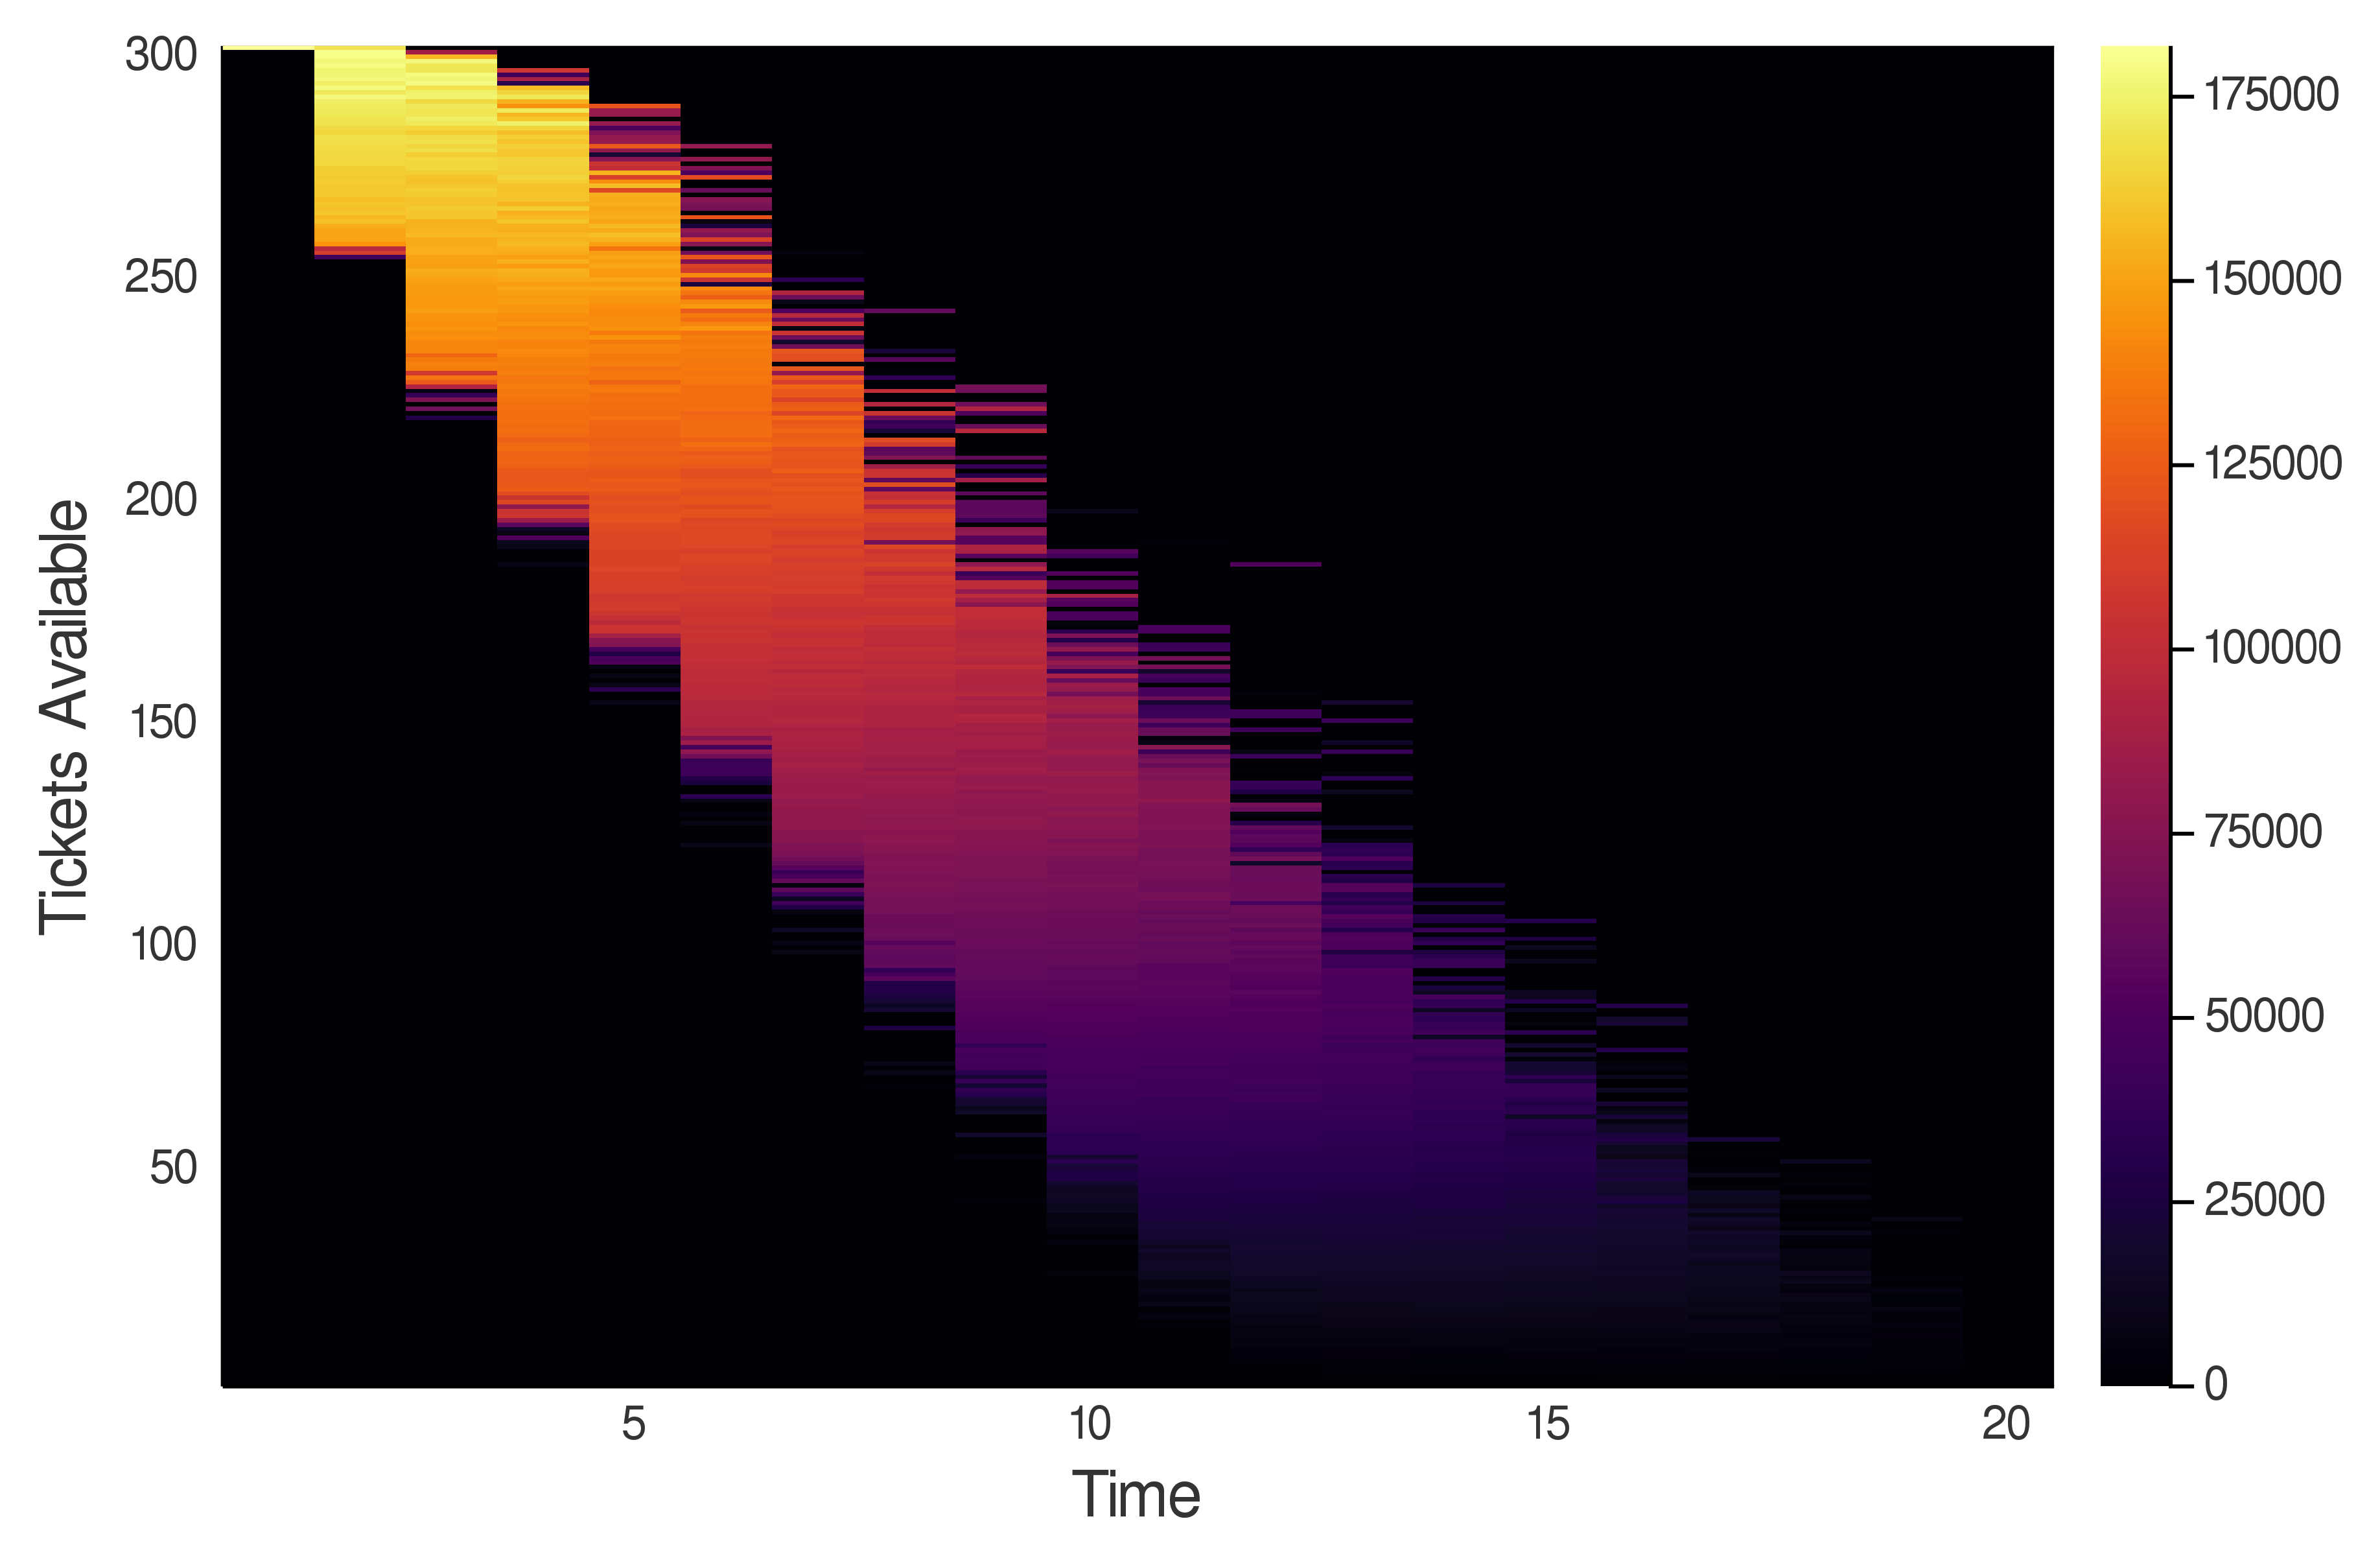
\includegraphics[width=0.48\linewidth]{final-paper/plots/singleAgentSarsa-U.png} \;
     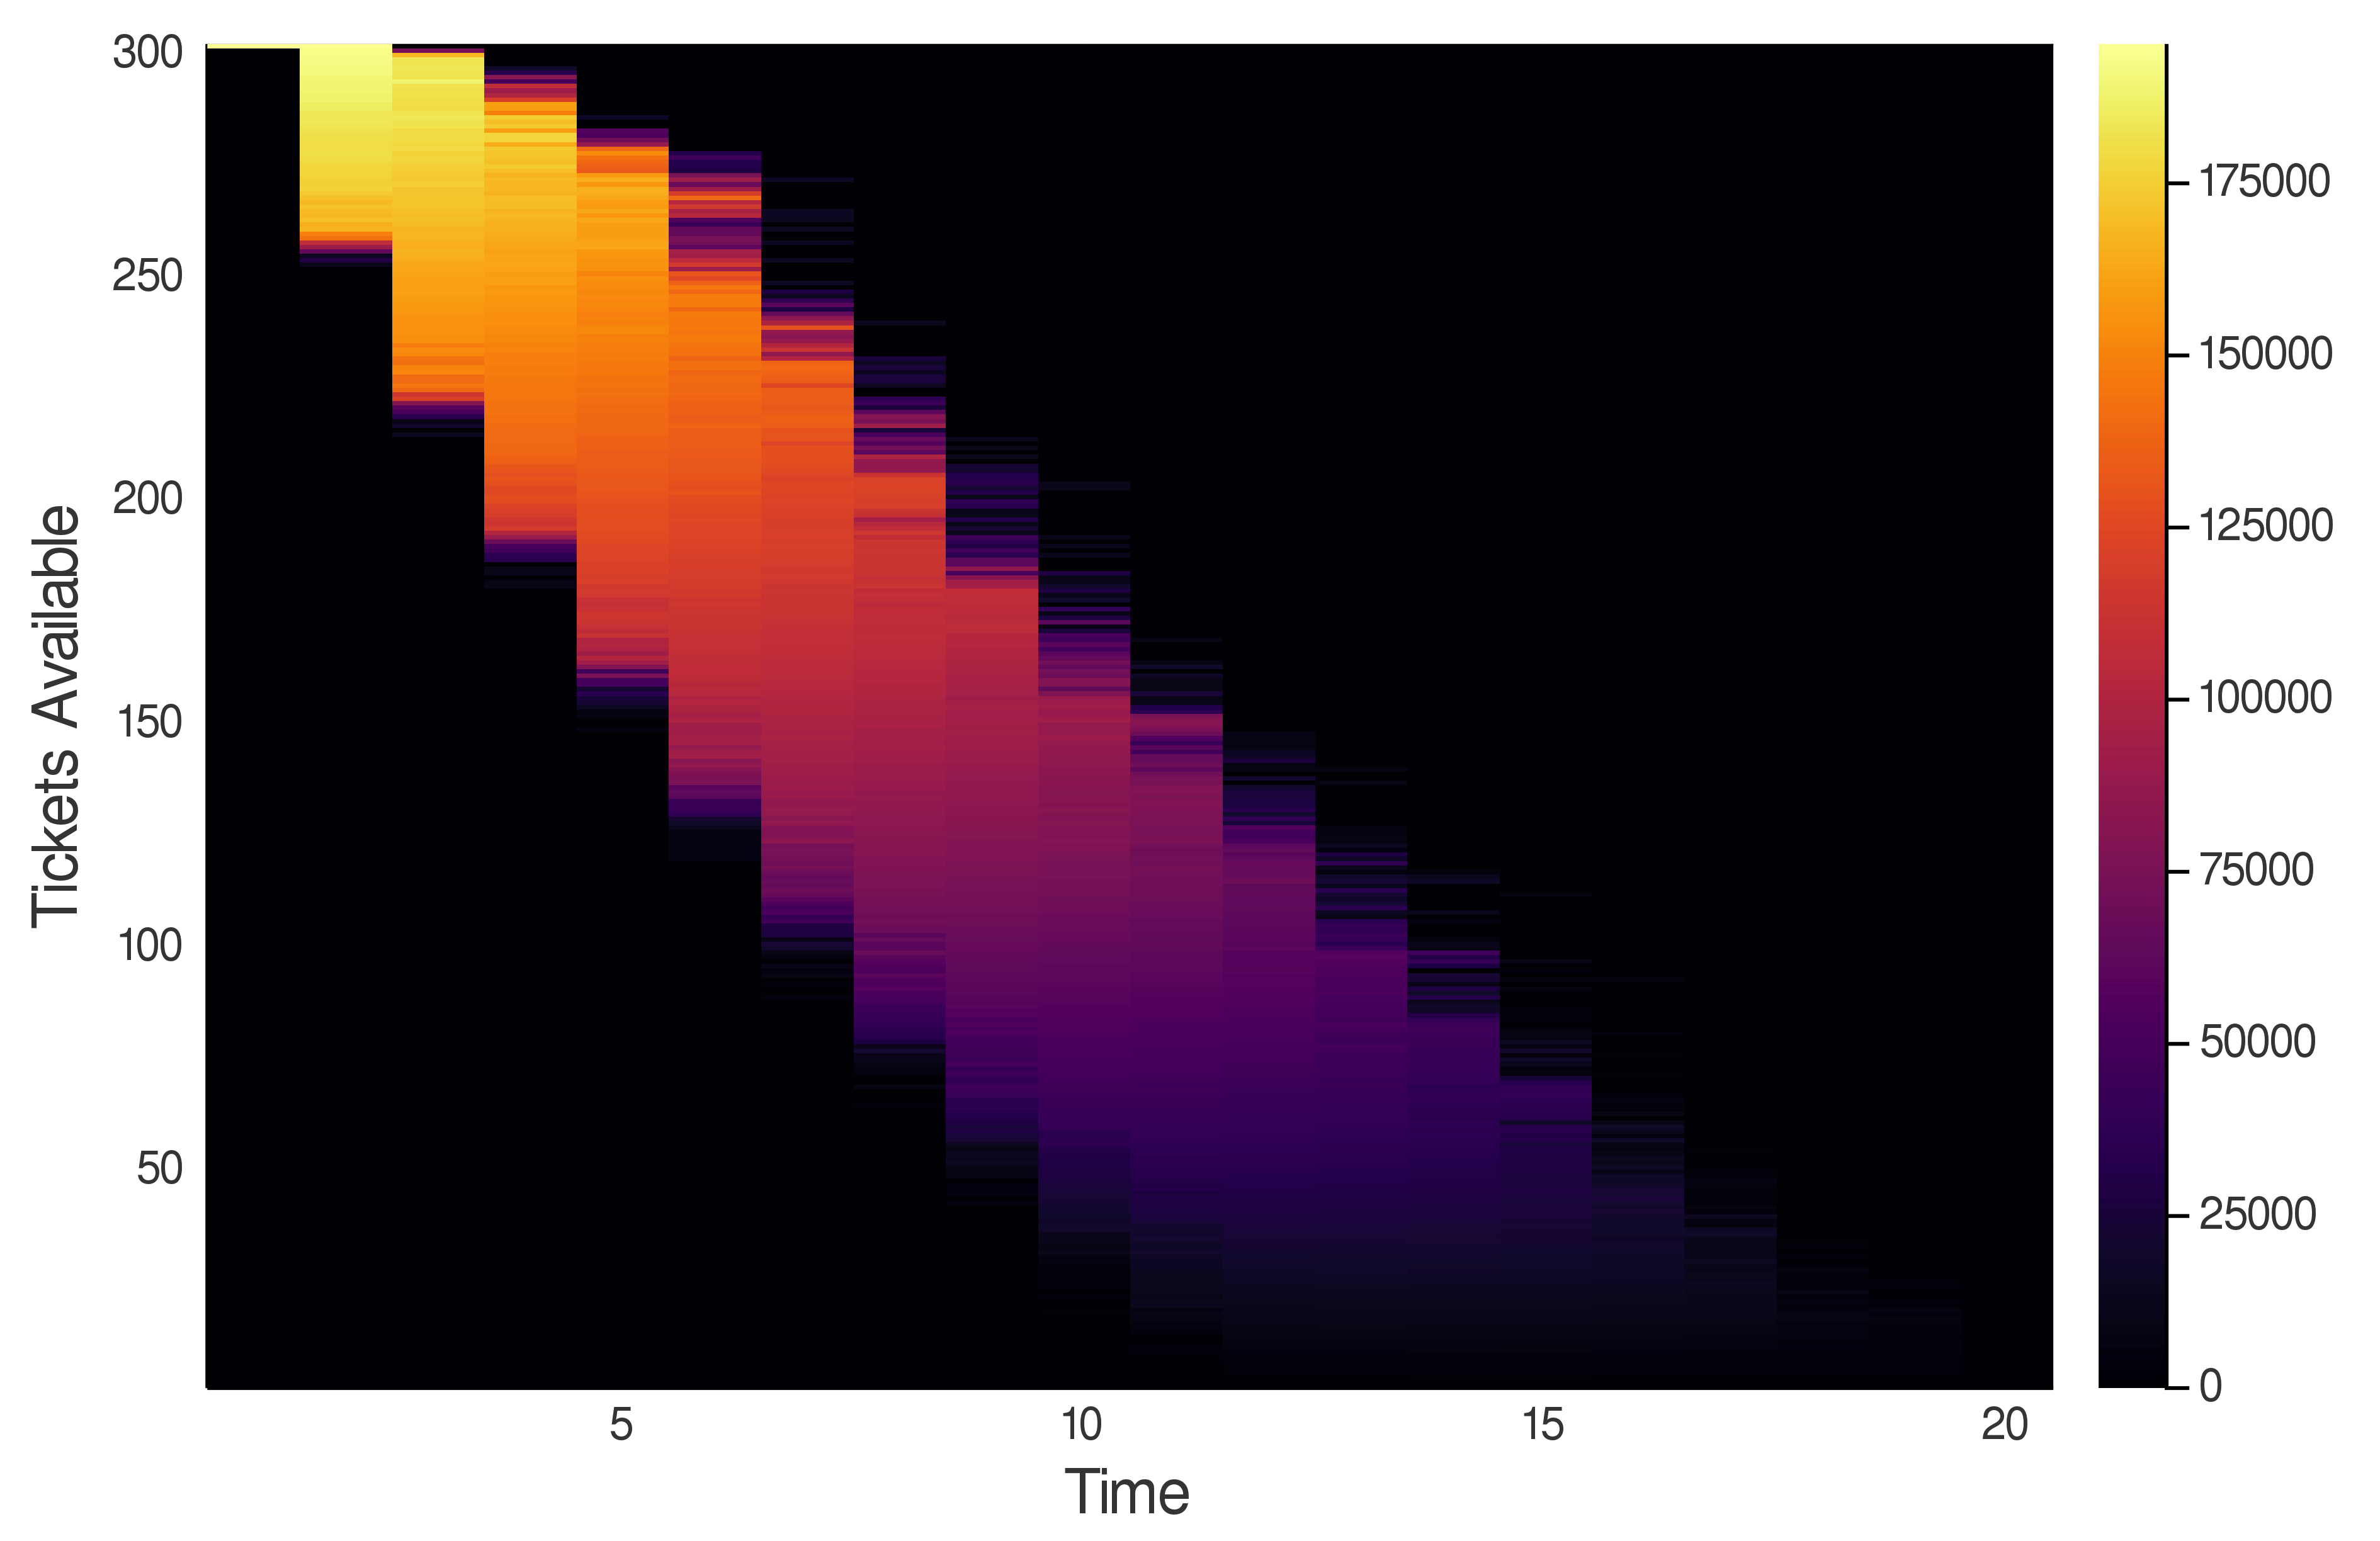
\includegraphics[width=0.48\linewidth]{final-paper/plots/singleAgentSarsaLambda-U.png}
    \caption{Optimal value functions for the single fare class case (fare class 1) trained using Sarsa (\textit{left}) and Sarsa($\lambda$) (\textit{right}).}
\end{figure}

\begin{figure}[h!]
    \centering
    \label{fig:single-class-sarsa-policy}
    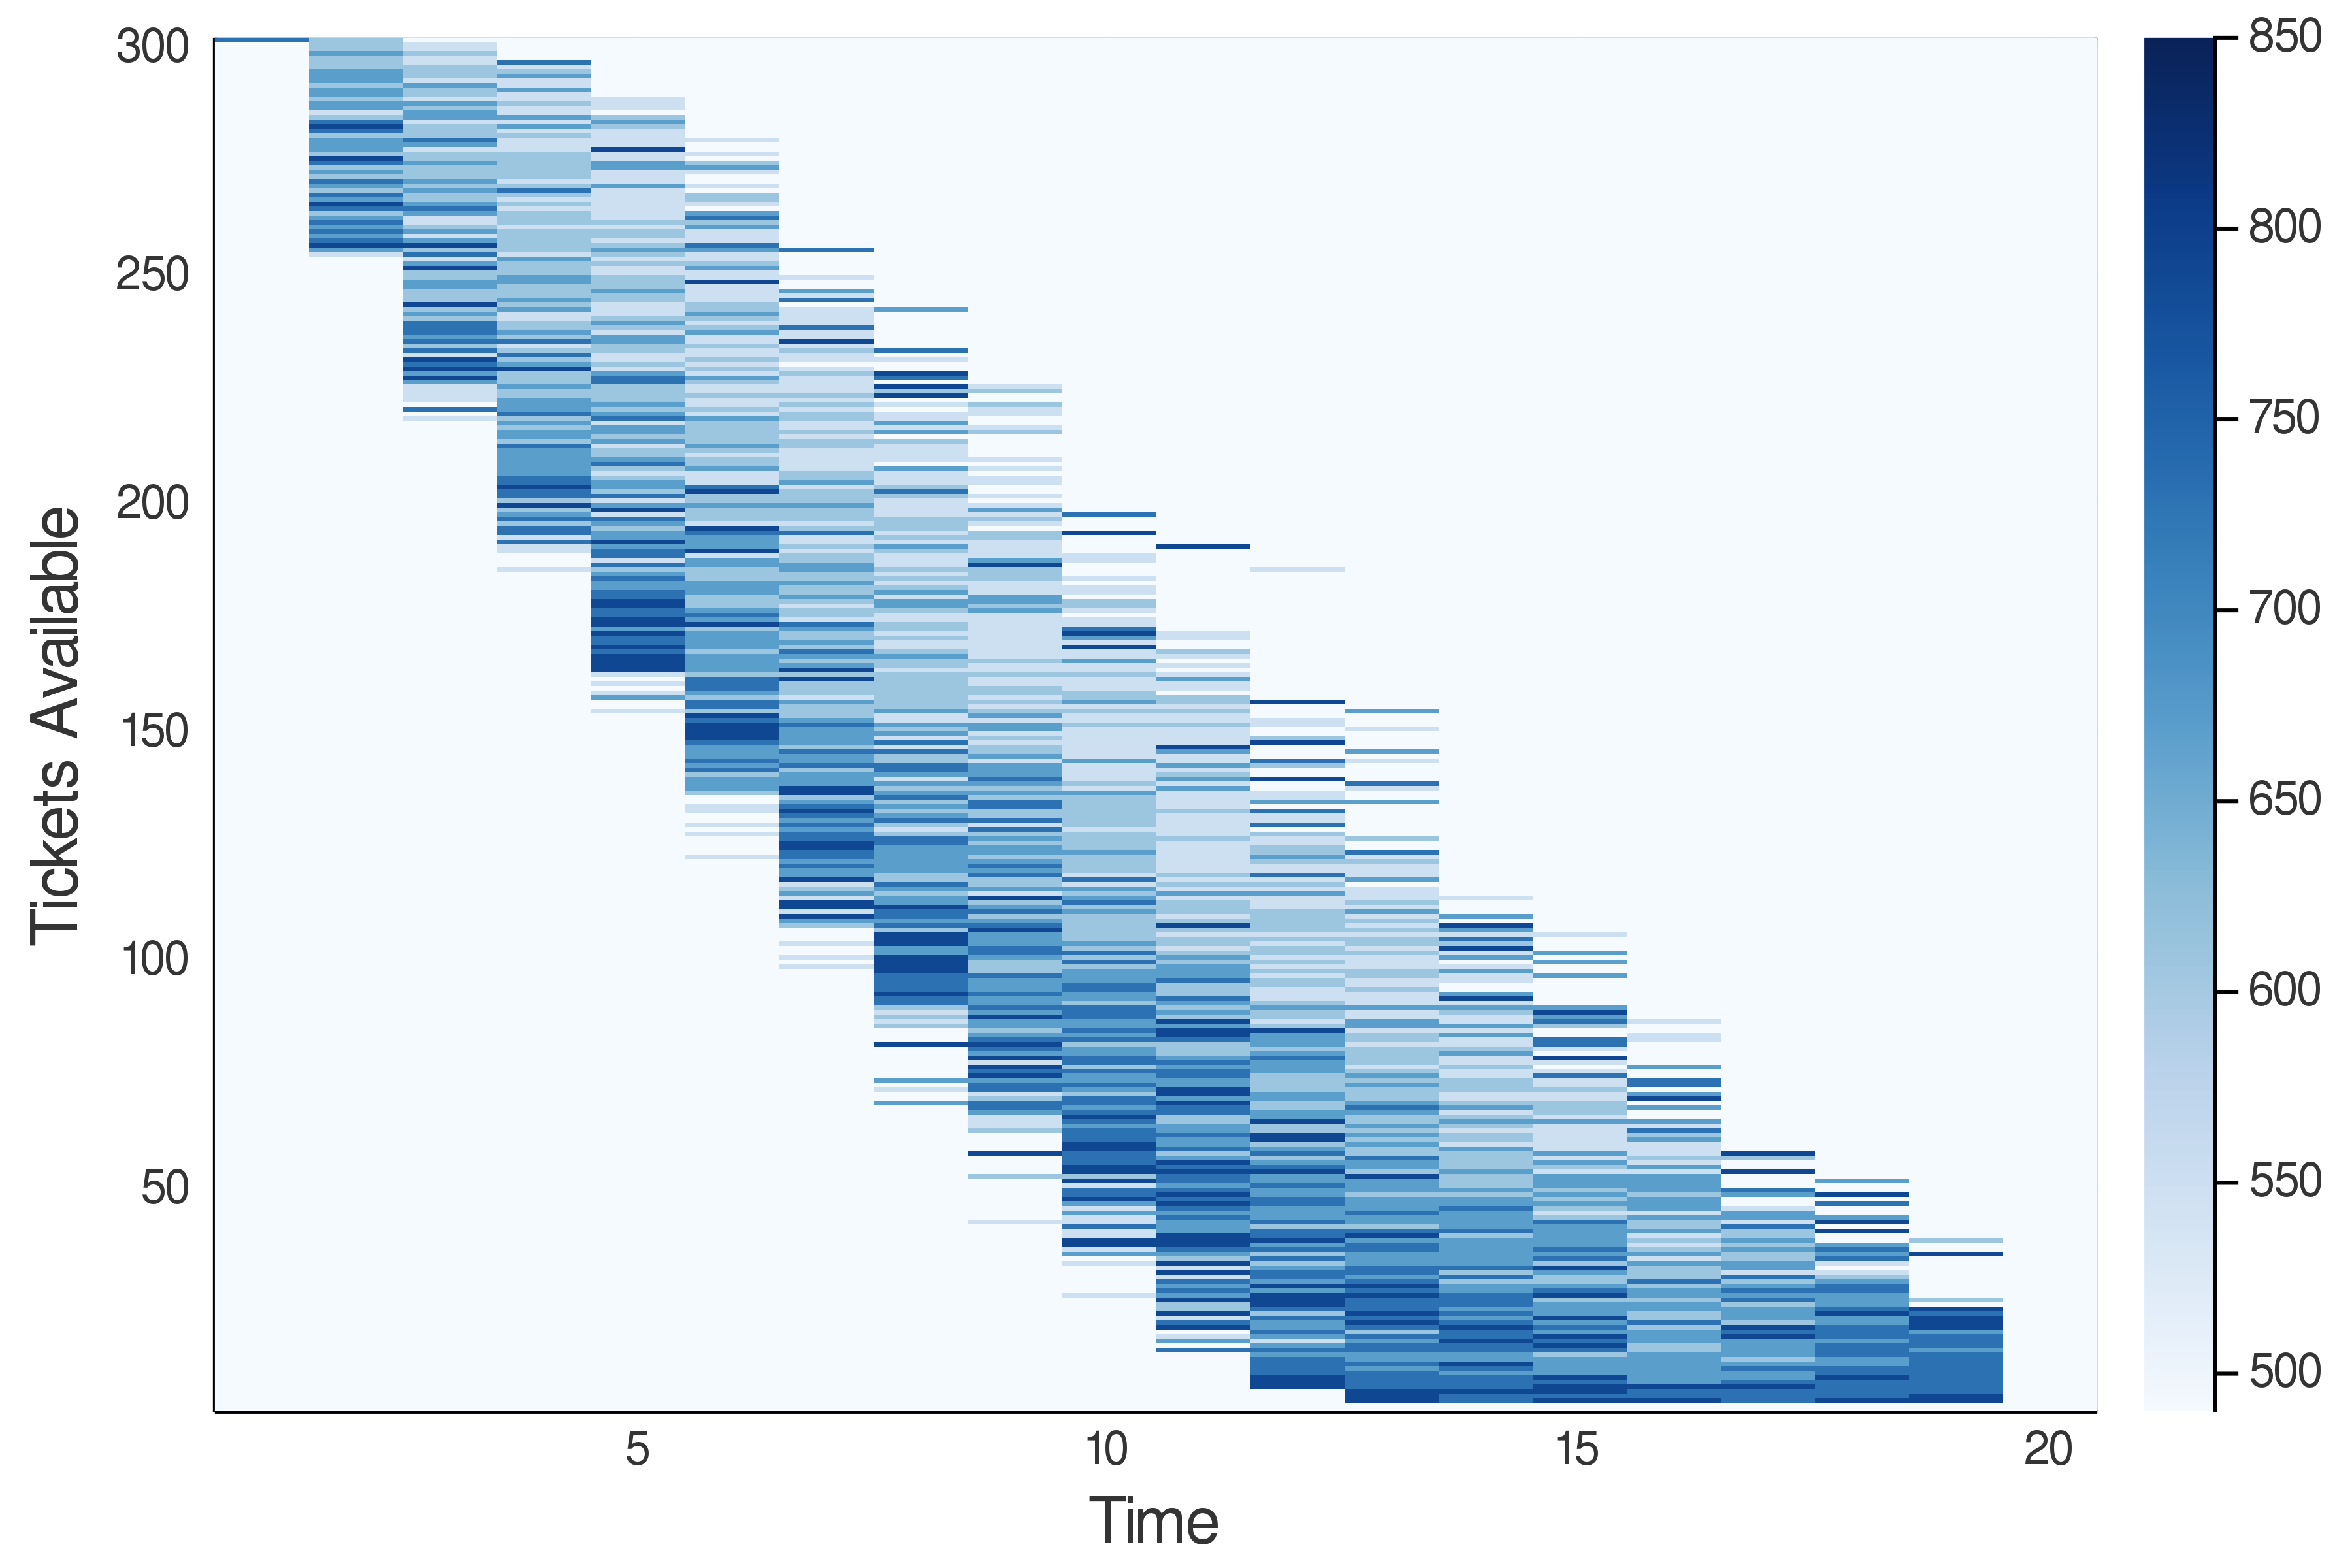
\includegraphics[width=0.48\linewidth]{final-paper/plots/singleAgentSarsa-policy.png} \;
    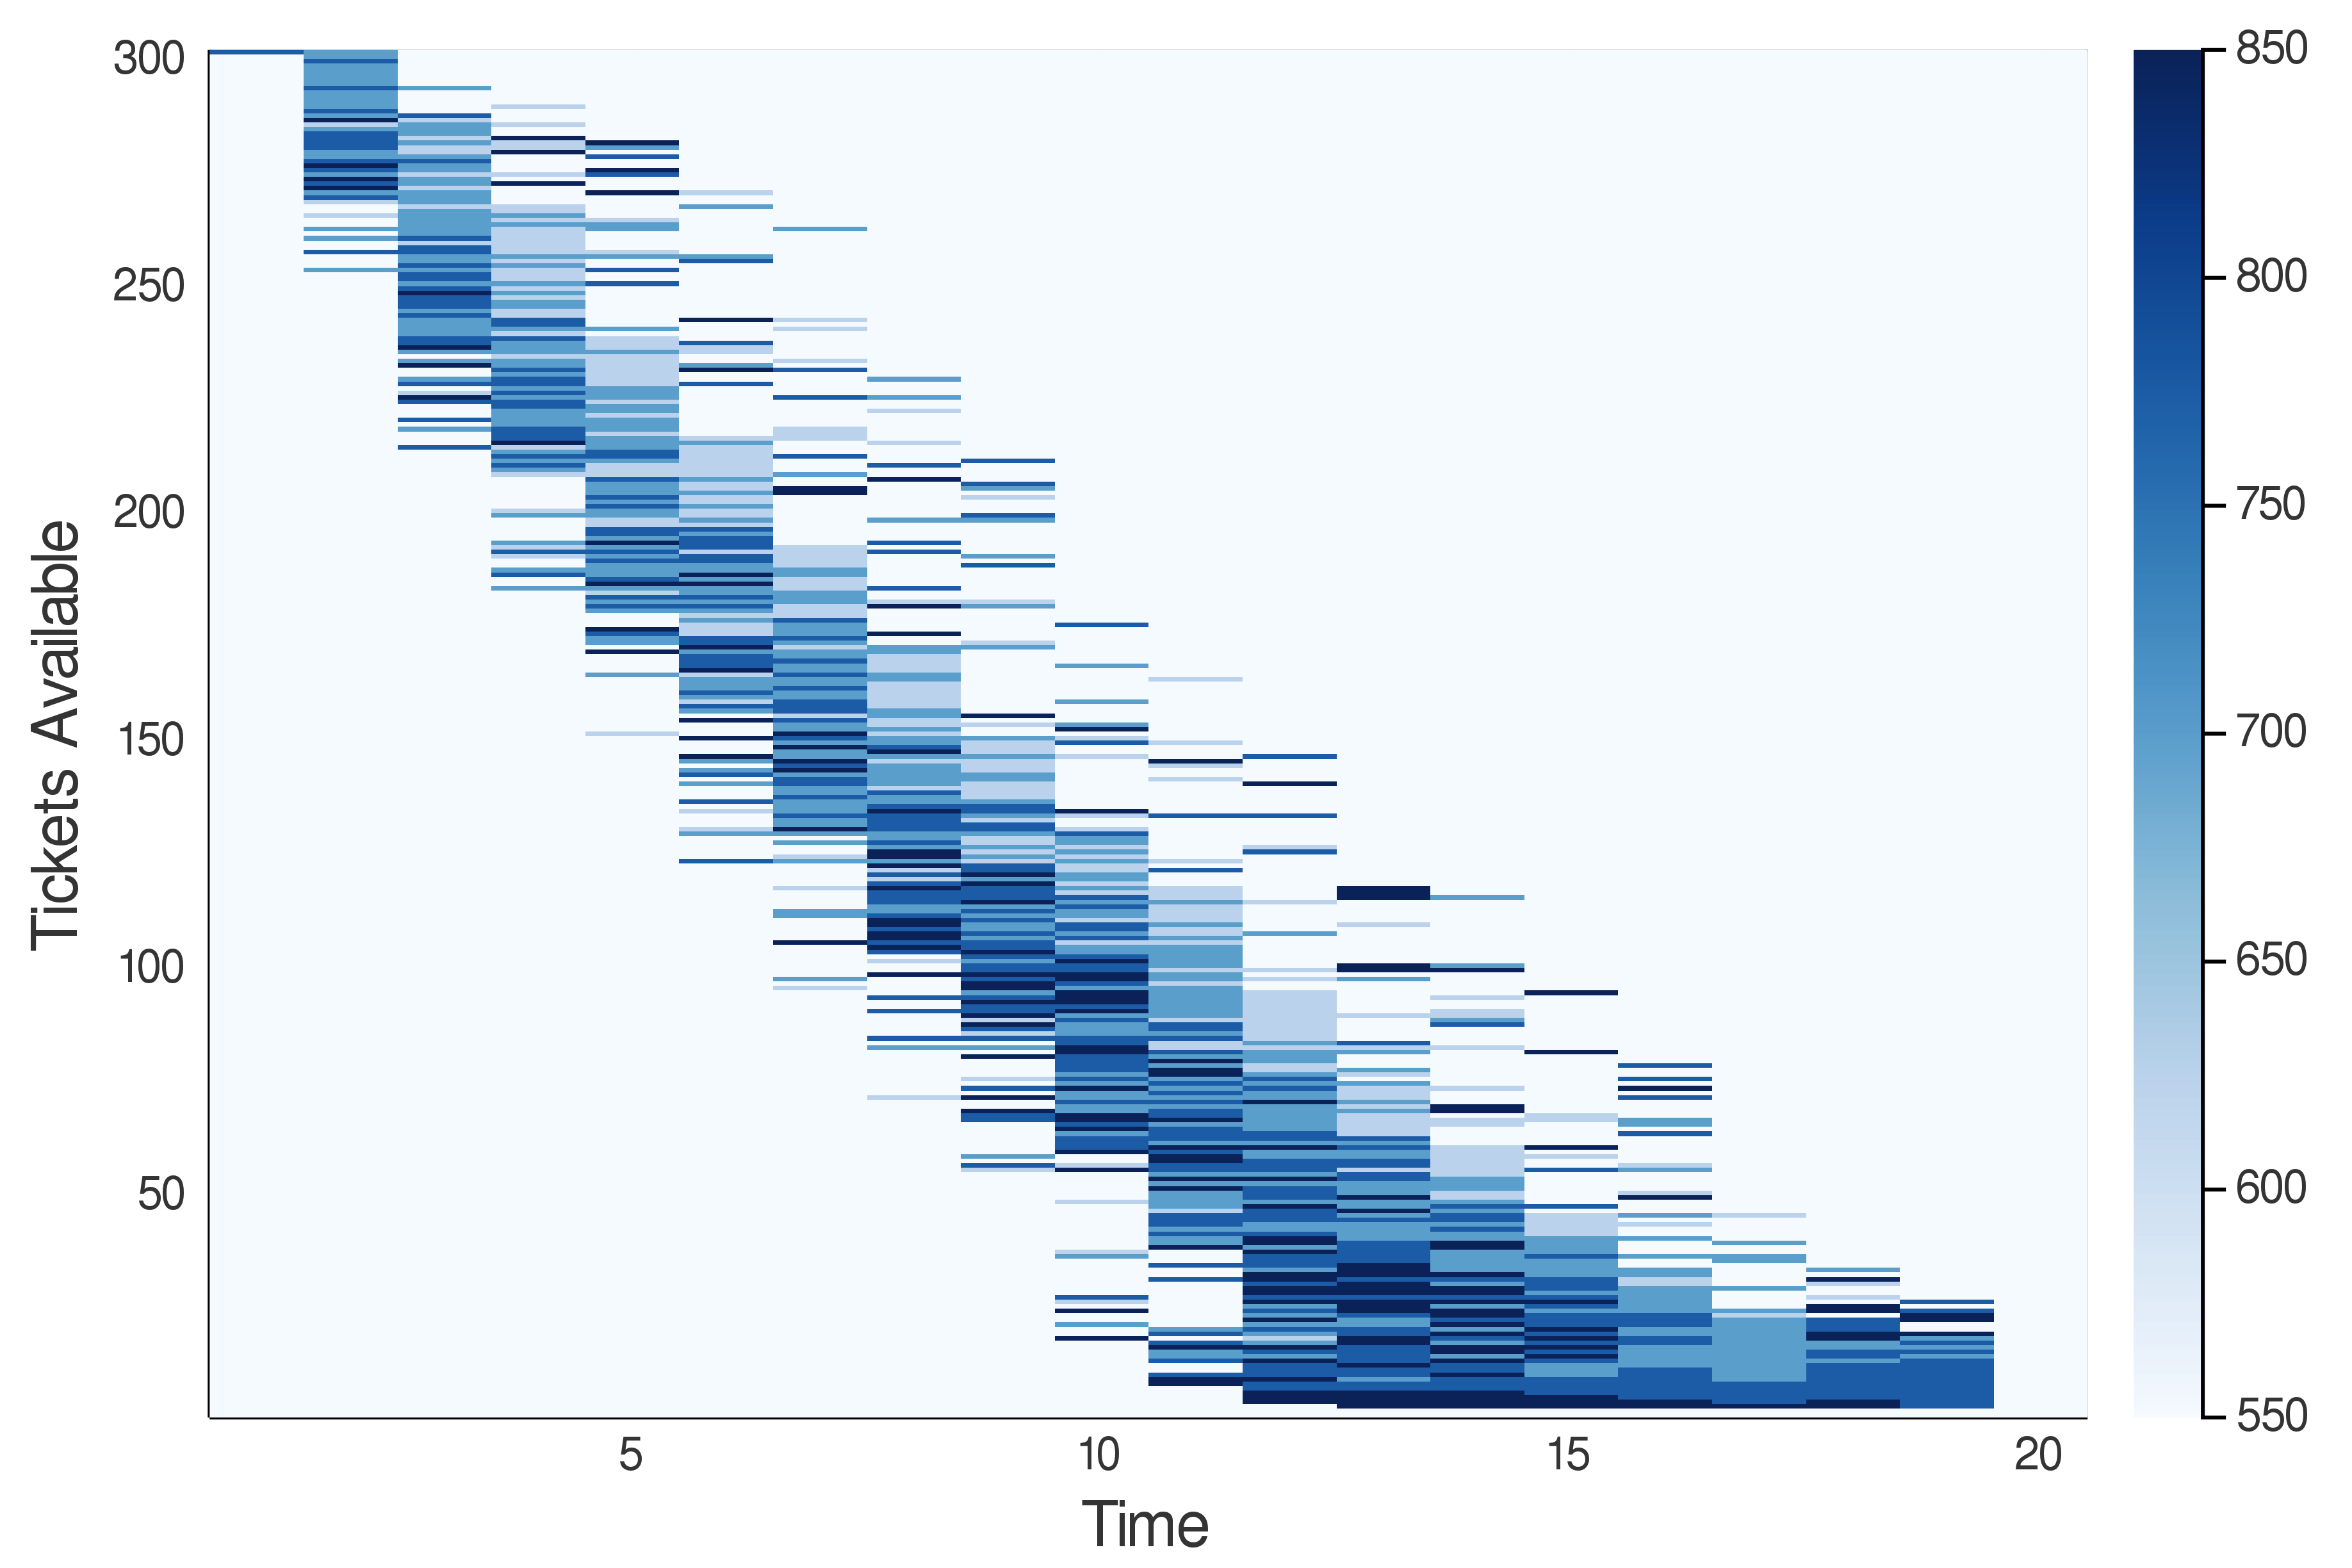
\includegraphics[width=0.48\linewidth]{final-paper/plots/singleAgentSarsaLambda-policy.png}
    \caption{Optimal pricing policies in dollars (\$) for the single fare class case (fare class 1) trained using Sarsa (\textit{left}) and Sarsa($\lambda$) (\textit{right}).}
\end{figure}

\begin{figure}[h!]
    \centering
    \label{fig:single-class-baselines-U}
    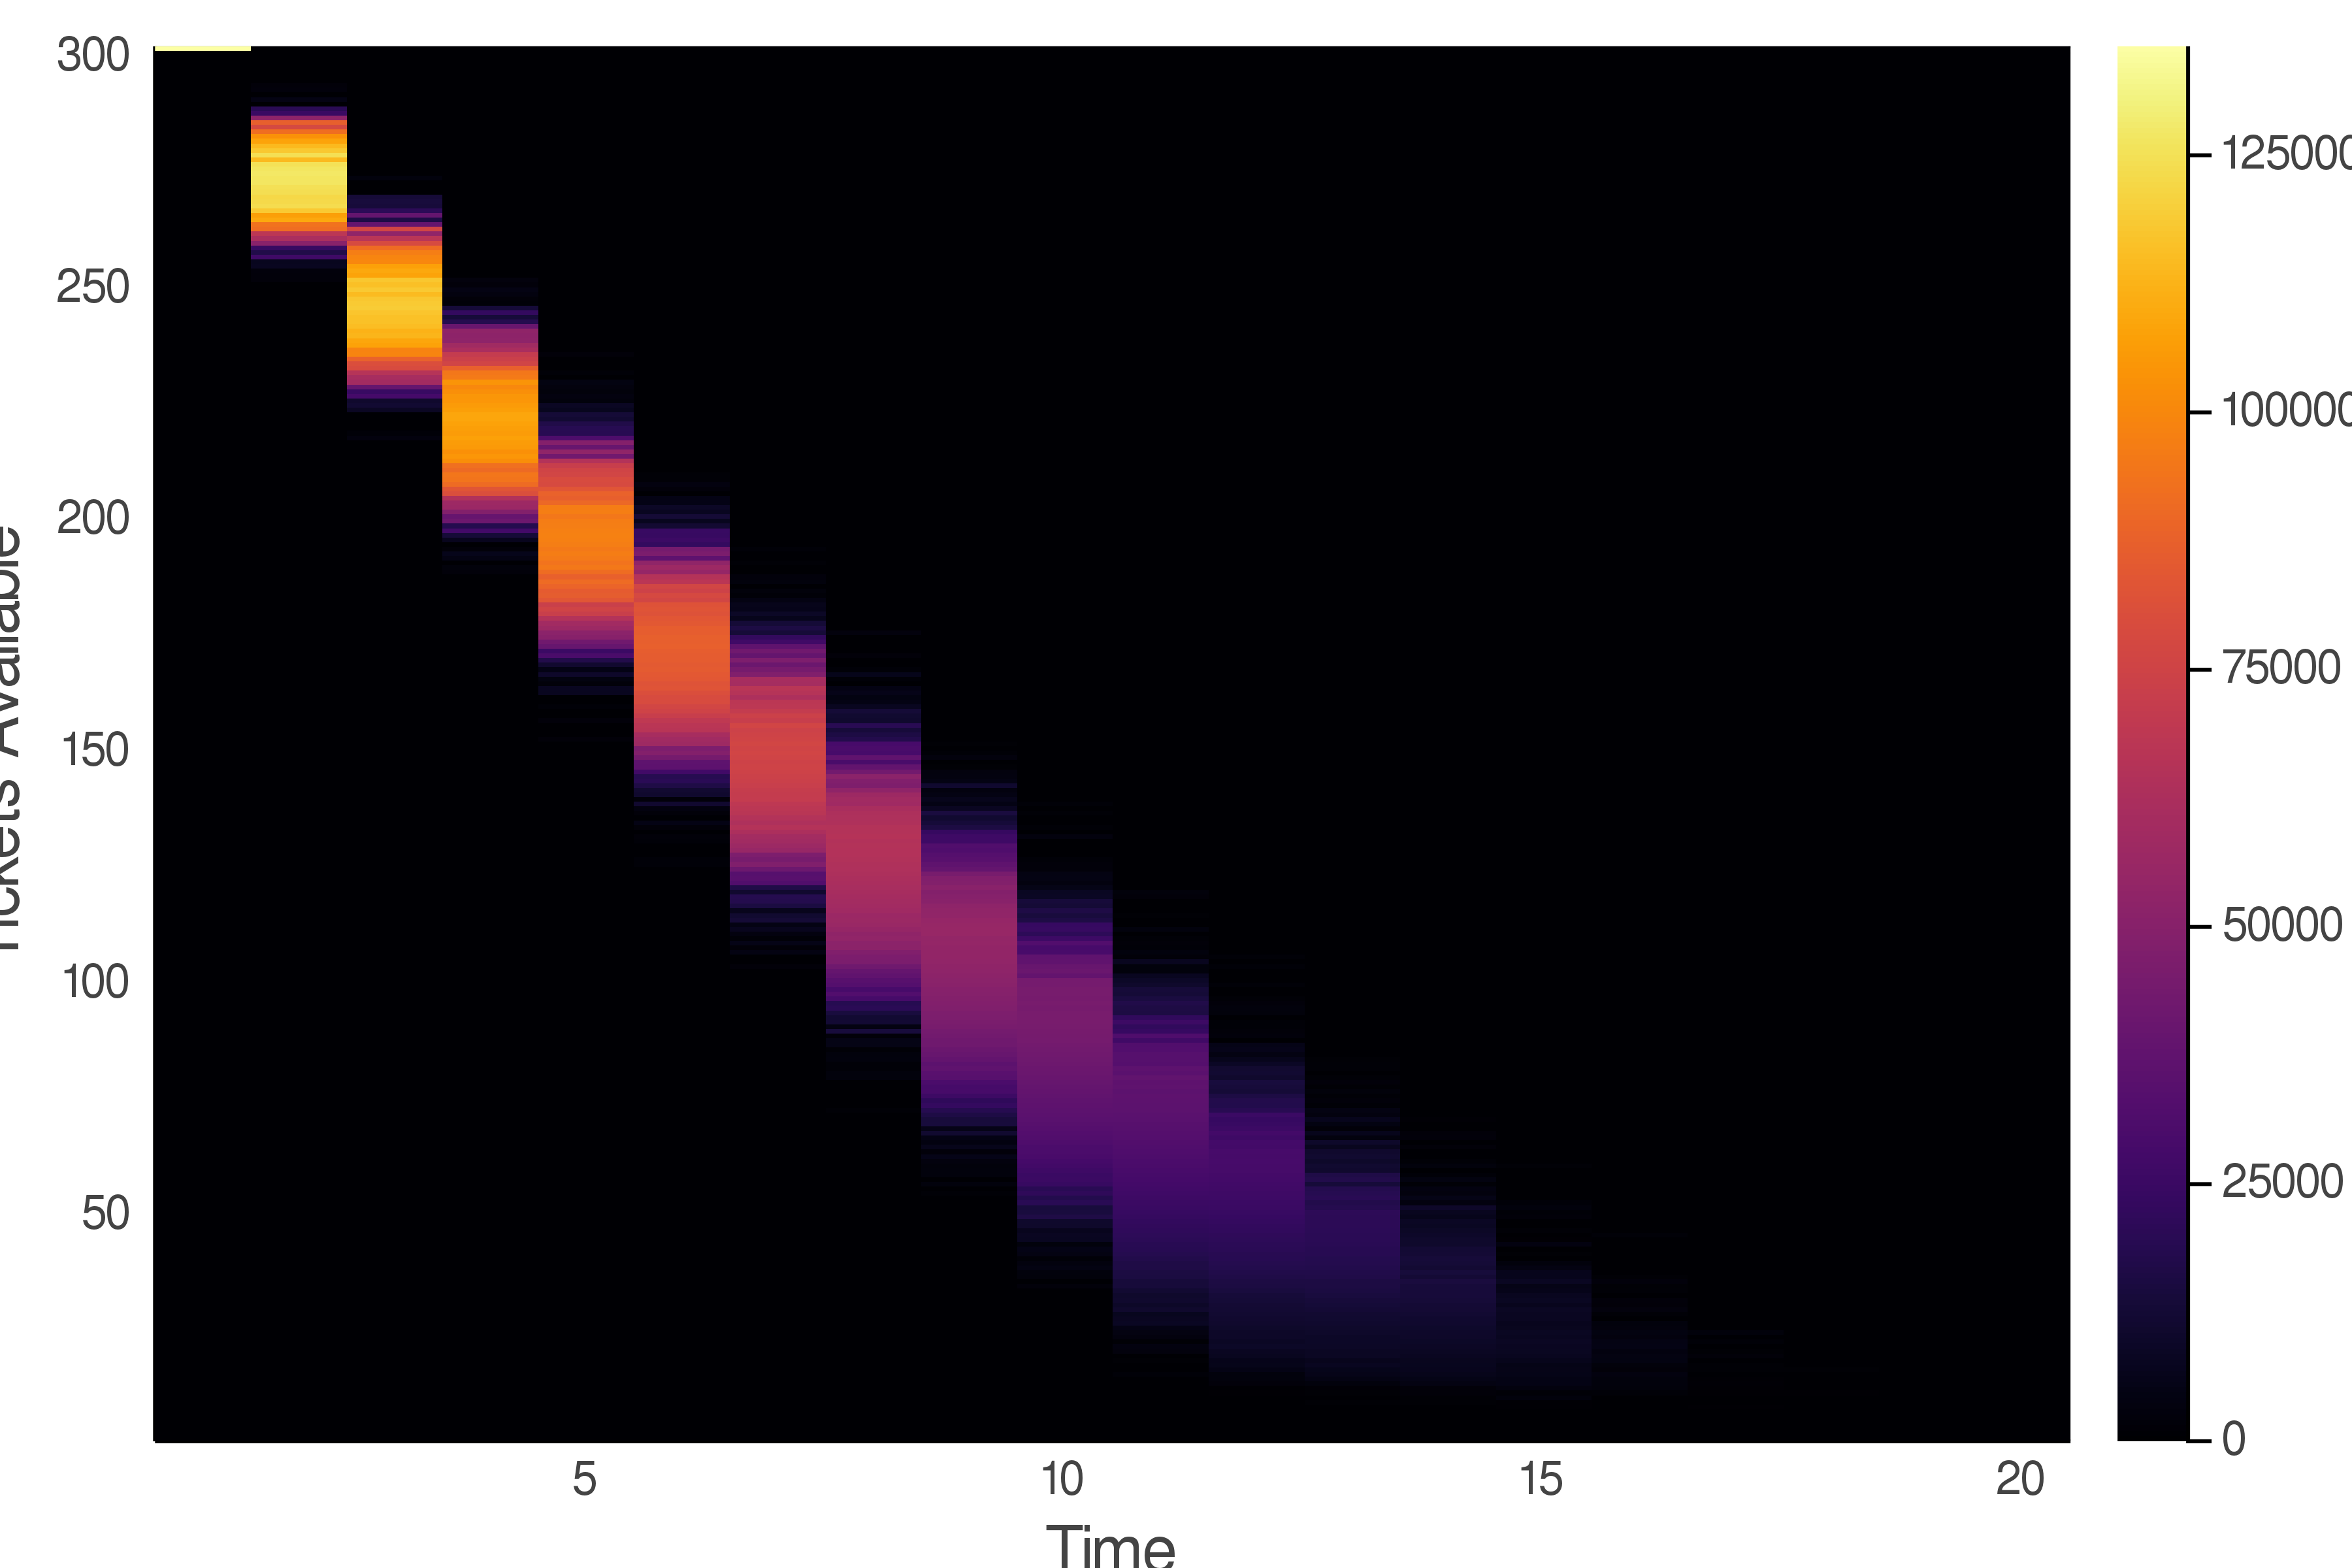
\includegraphics[width=0.3\linewidth]{final-paper/plots/singleAgentStaticLow-U.png} \;
    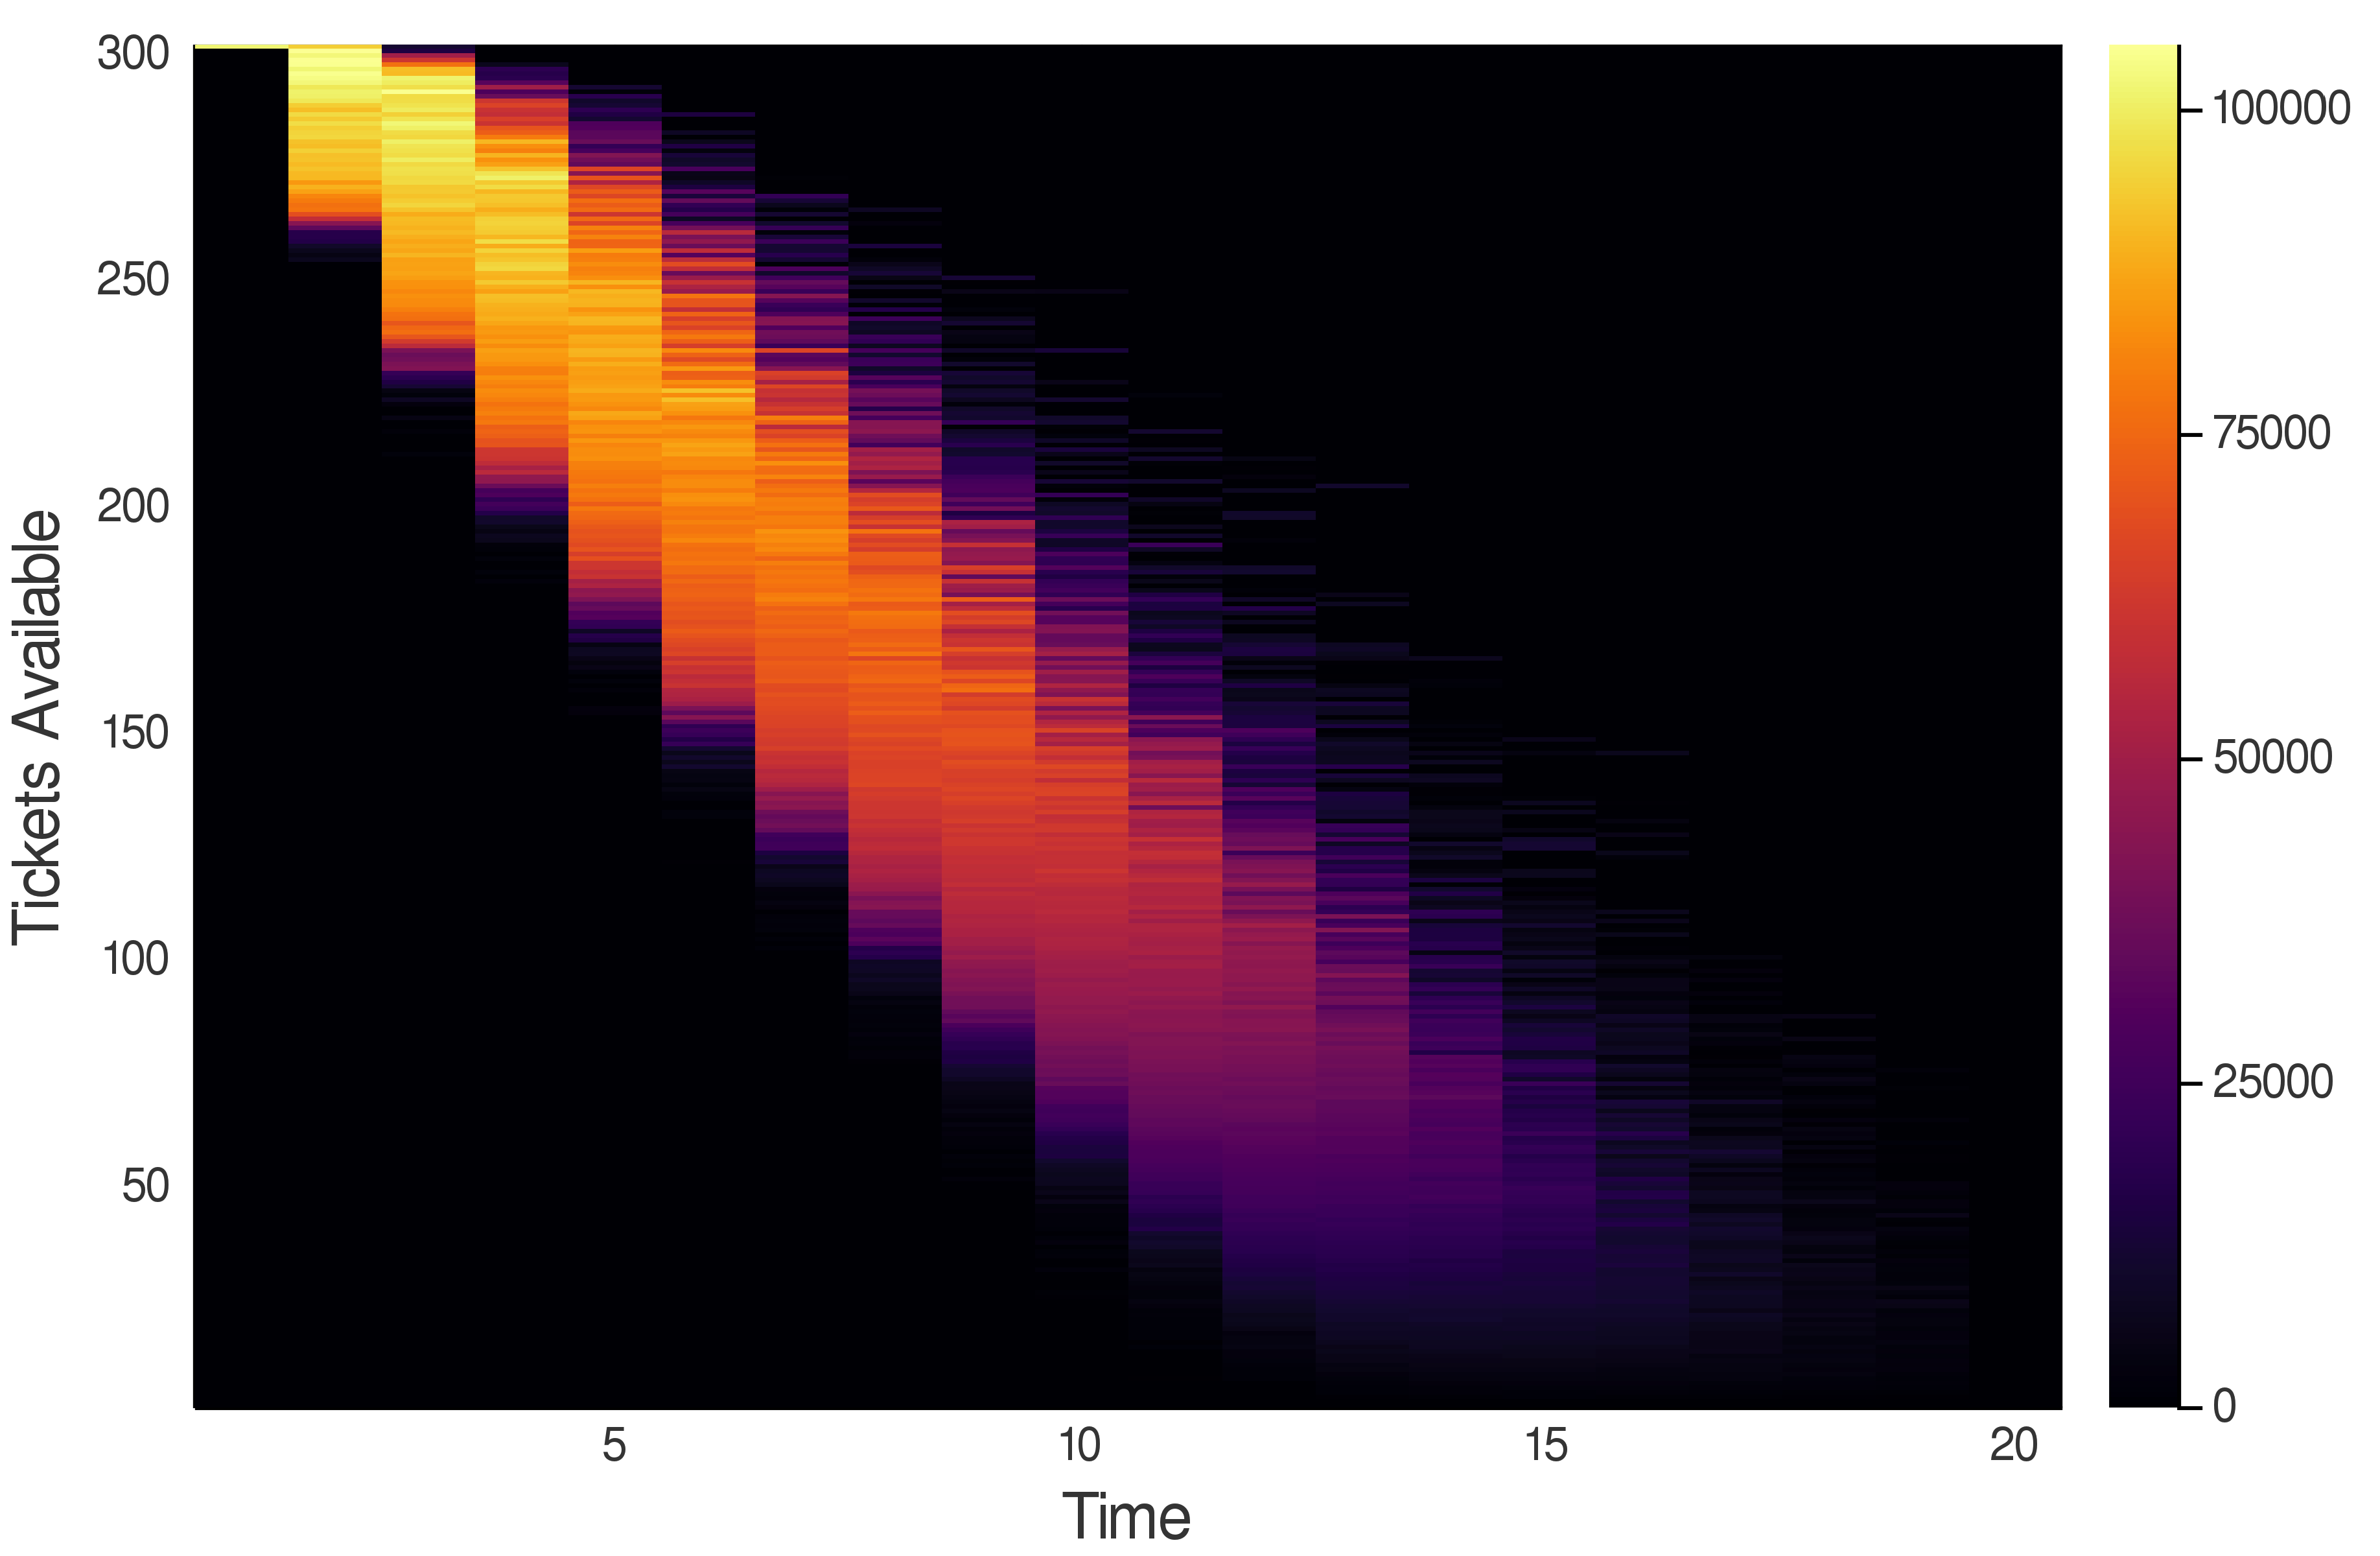
\includegraphics[width=0.3\linewidth]{final-paper/plots/singleAgentRandom-U.png} \;
    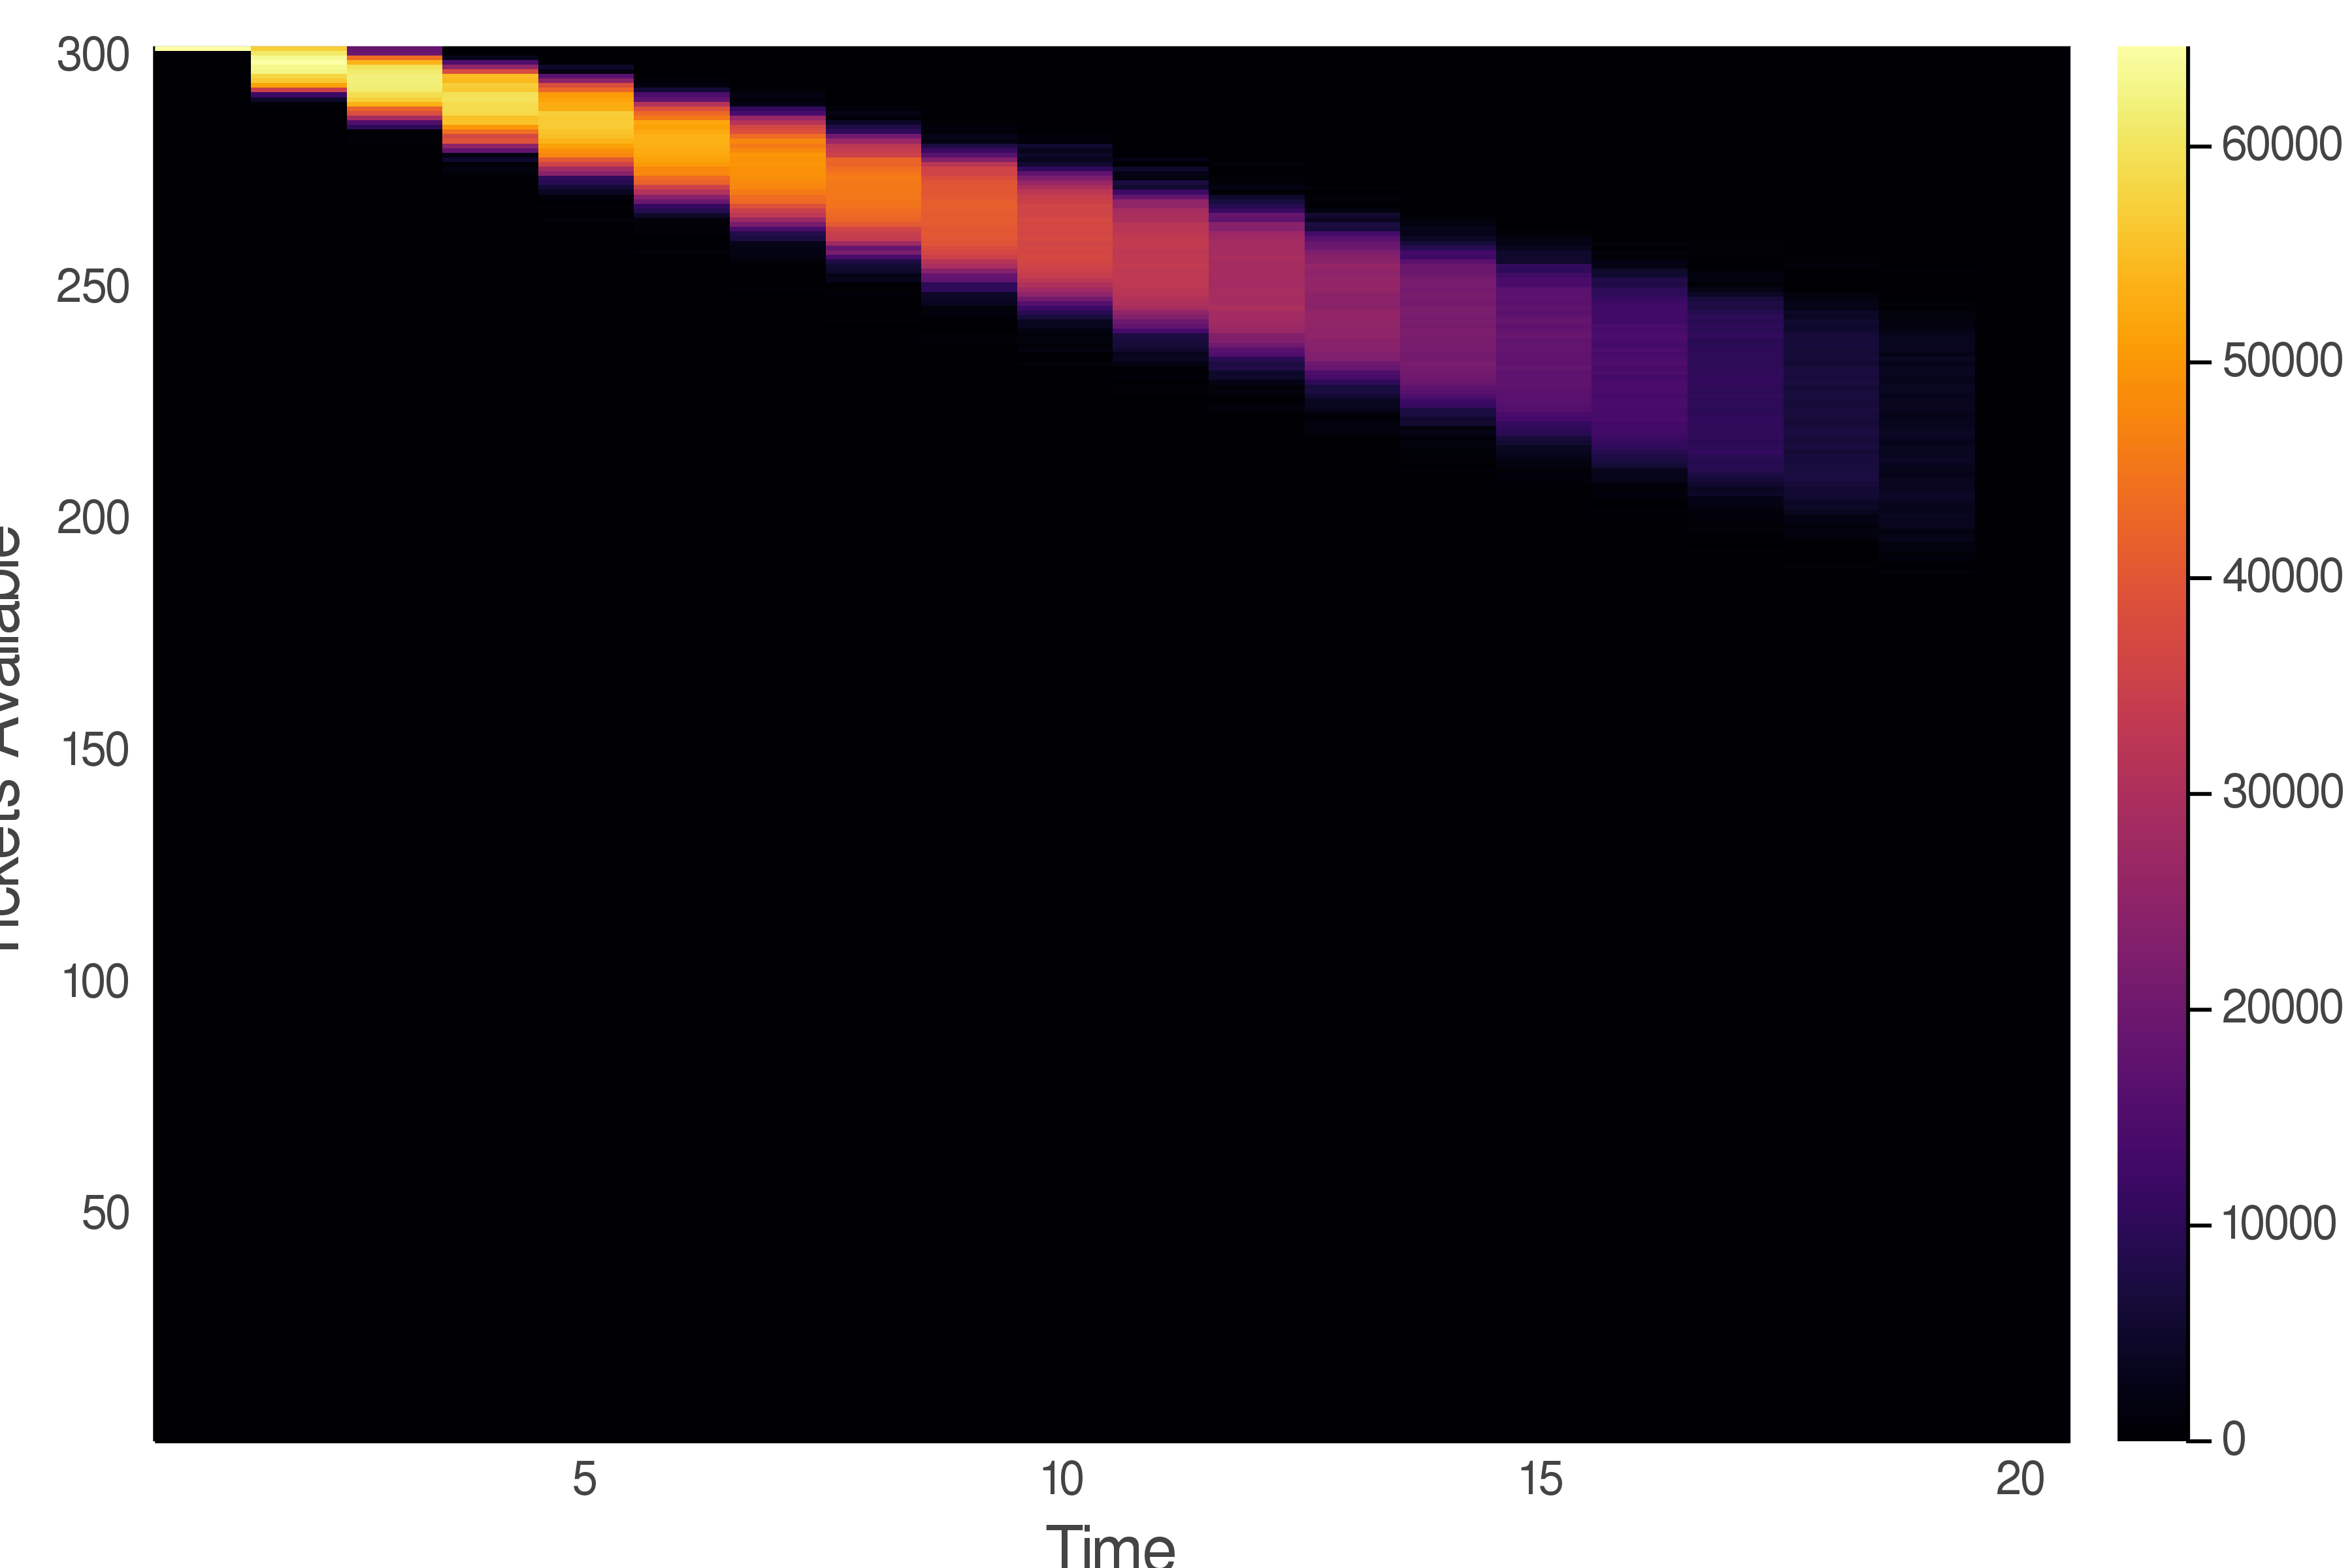
\includegraphics[width=0.3\linewidth]{final-paper/plots/singleAgentStaticHigh-U.png}
    \caption{Optimal value functions for the single fare class case (fare class 1) using the cheapest price (\textit{left}), a random policy (\textit{center}), and the most expensive price (\textit{right}).}
\end{figure}

\begin{figure}[h!]
    \centering
    \label{fig:single-class-baselines-policy}
    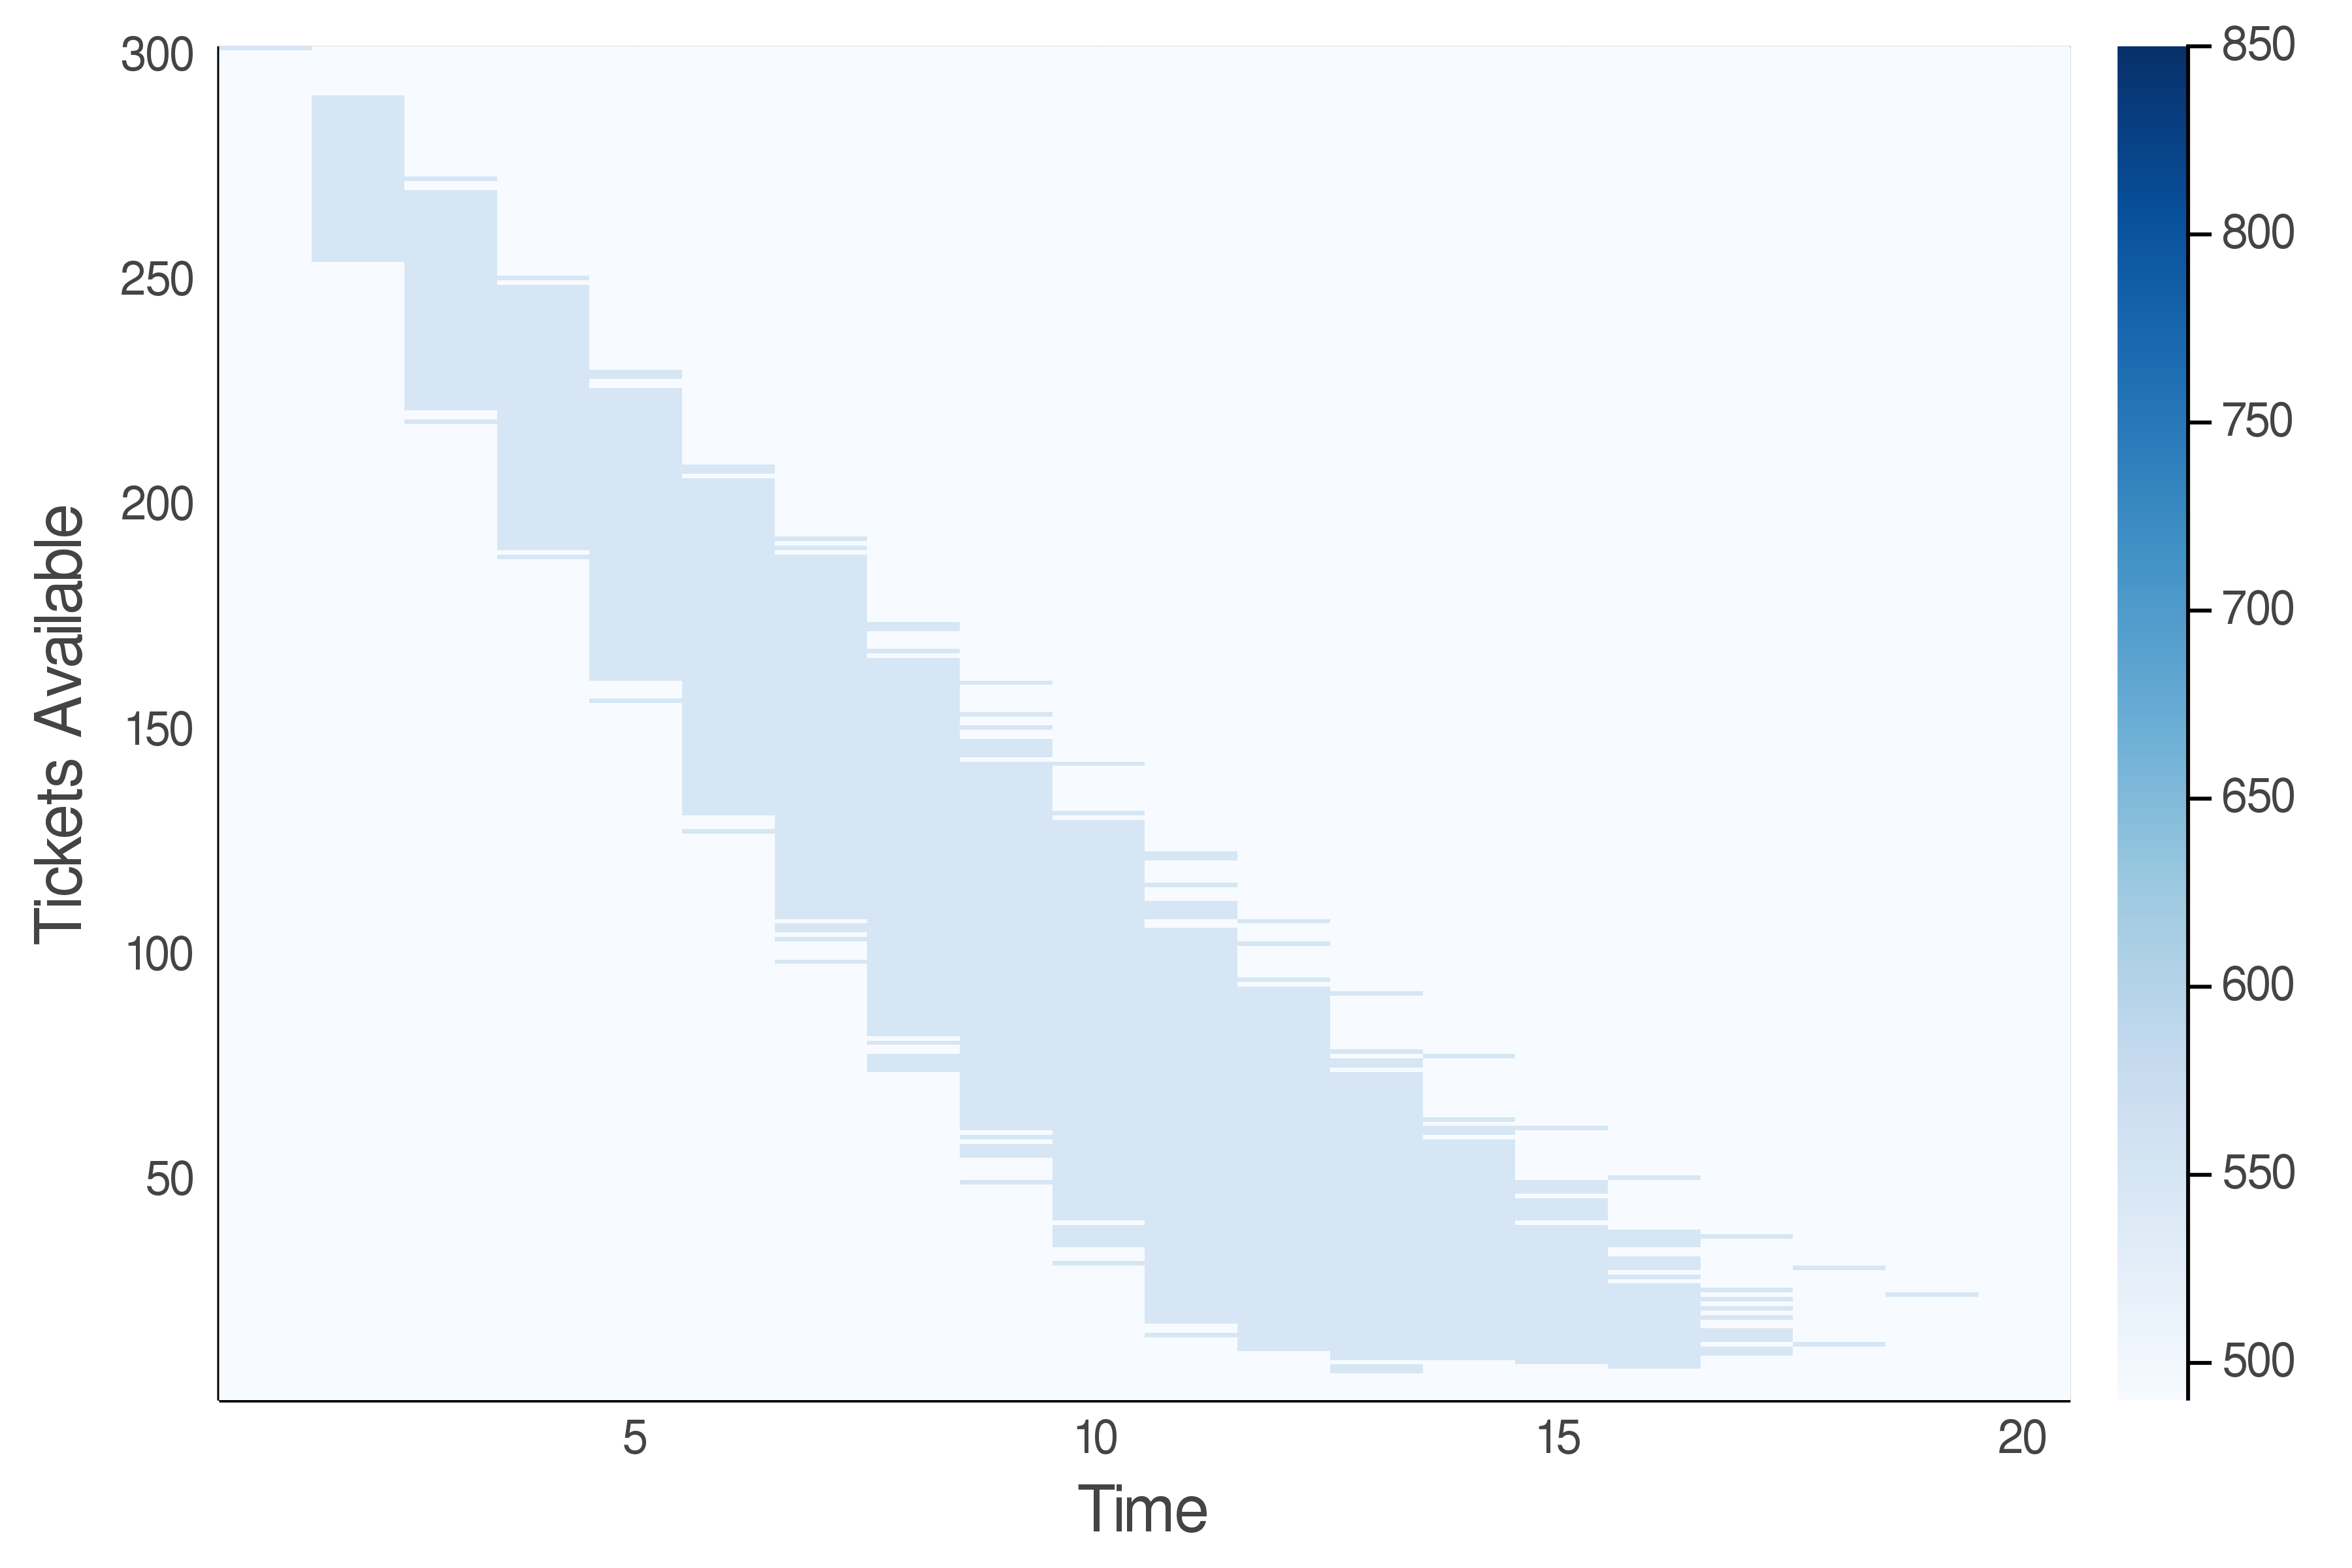
\includegraphics[width=0.3\linewidth]{final-paper/plots/singleAgentStaticLow-policy.png} \;
    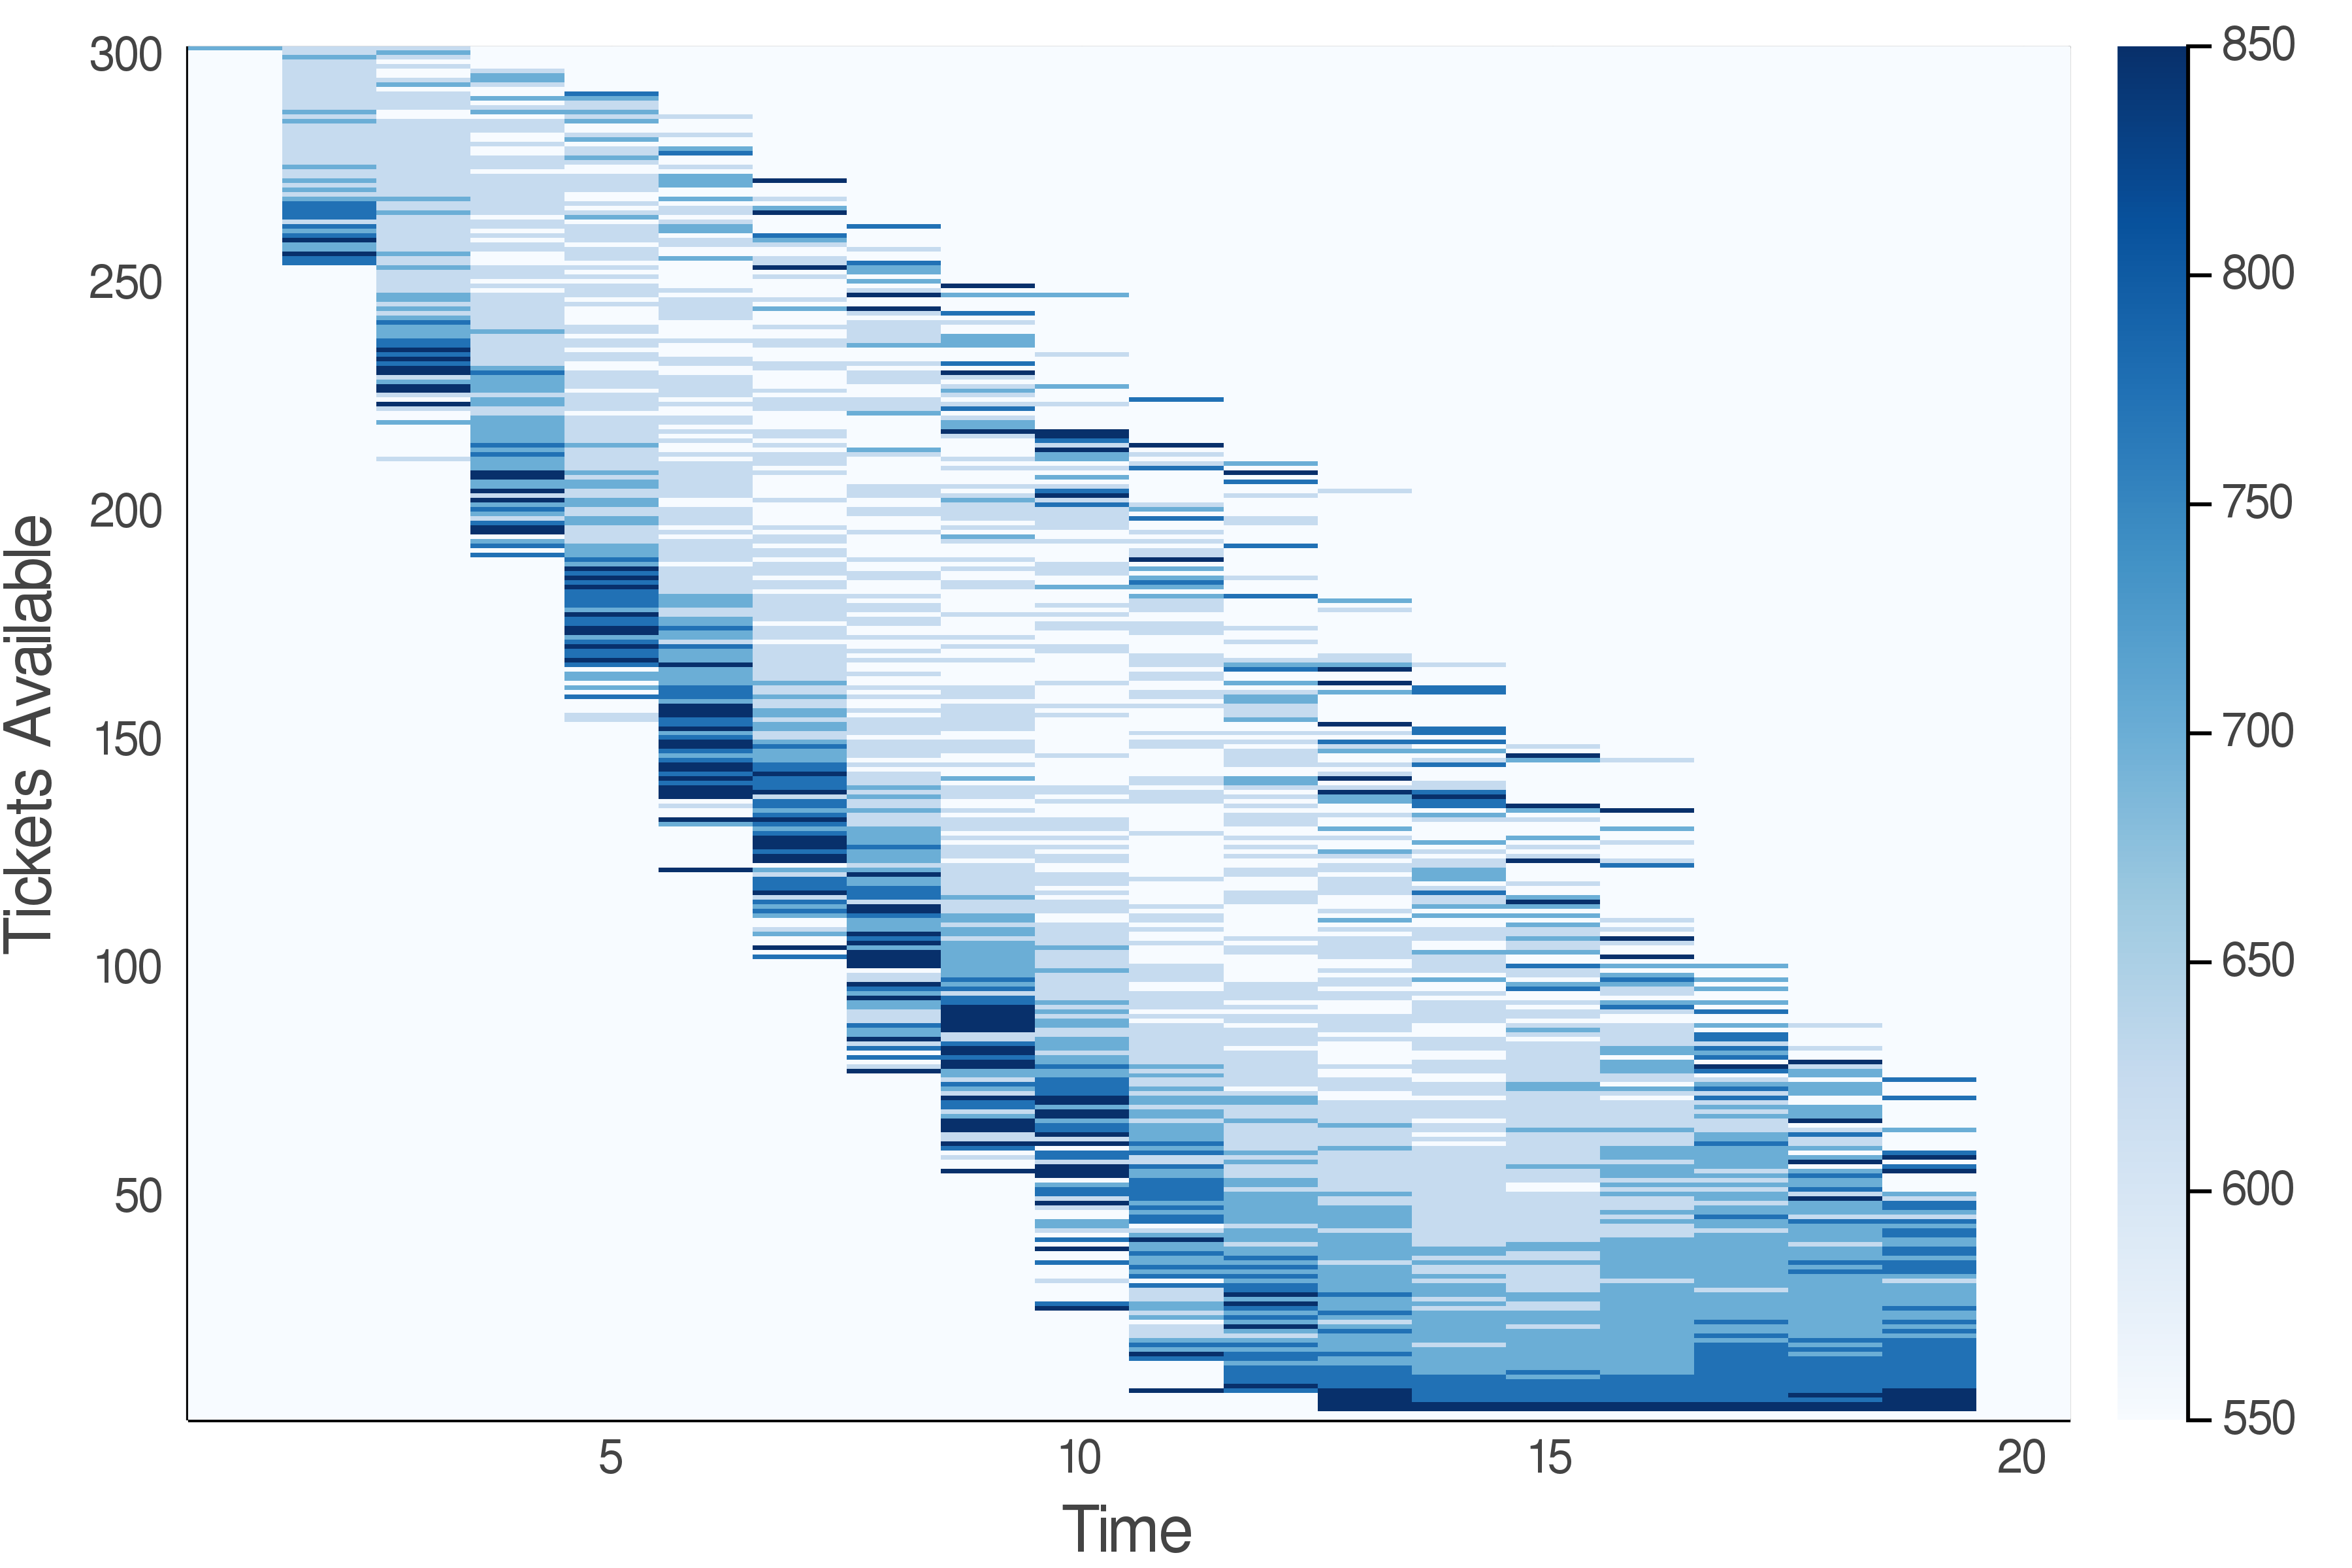
\includegraphics[width=0.3\linewidth]{final-paper/plots/singleAgentRandom-policy.png} \;
    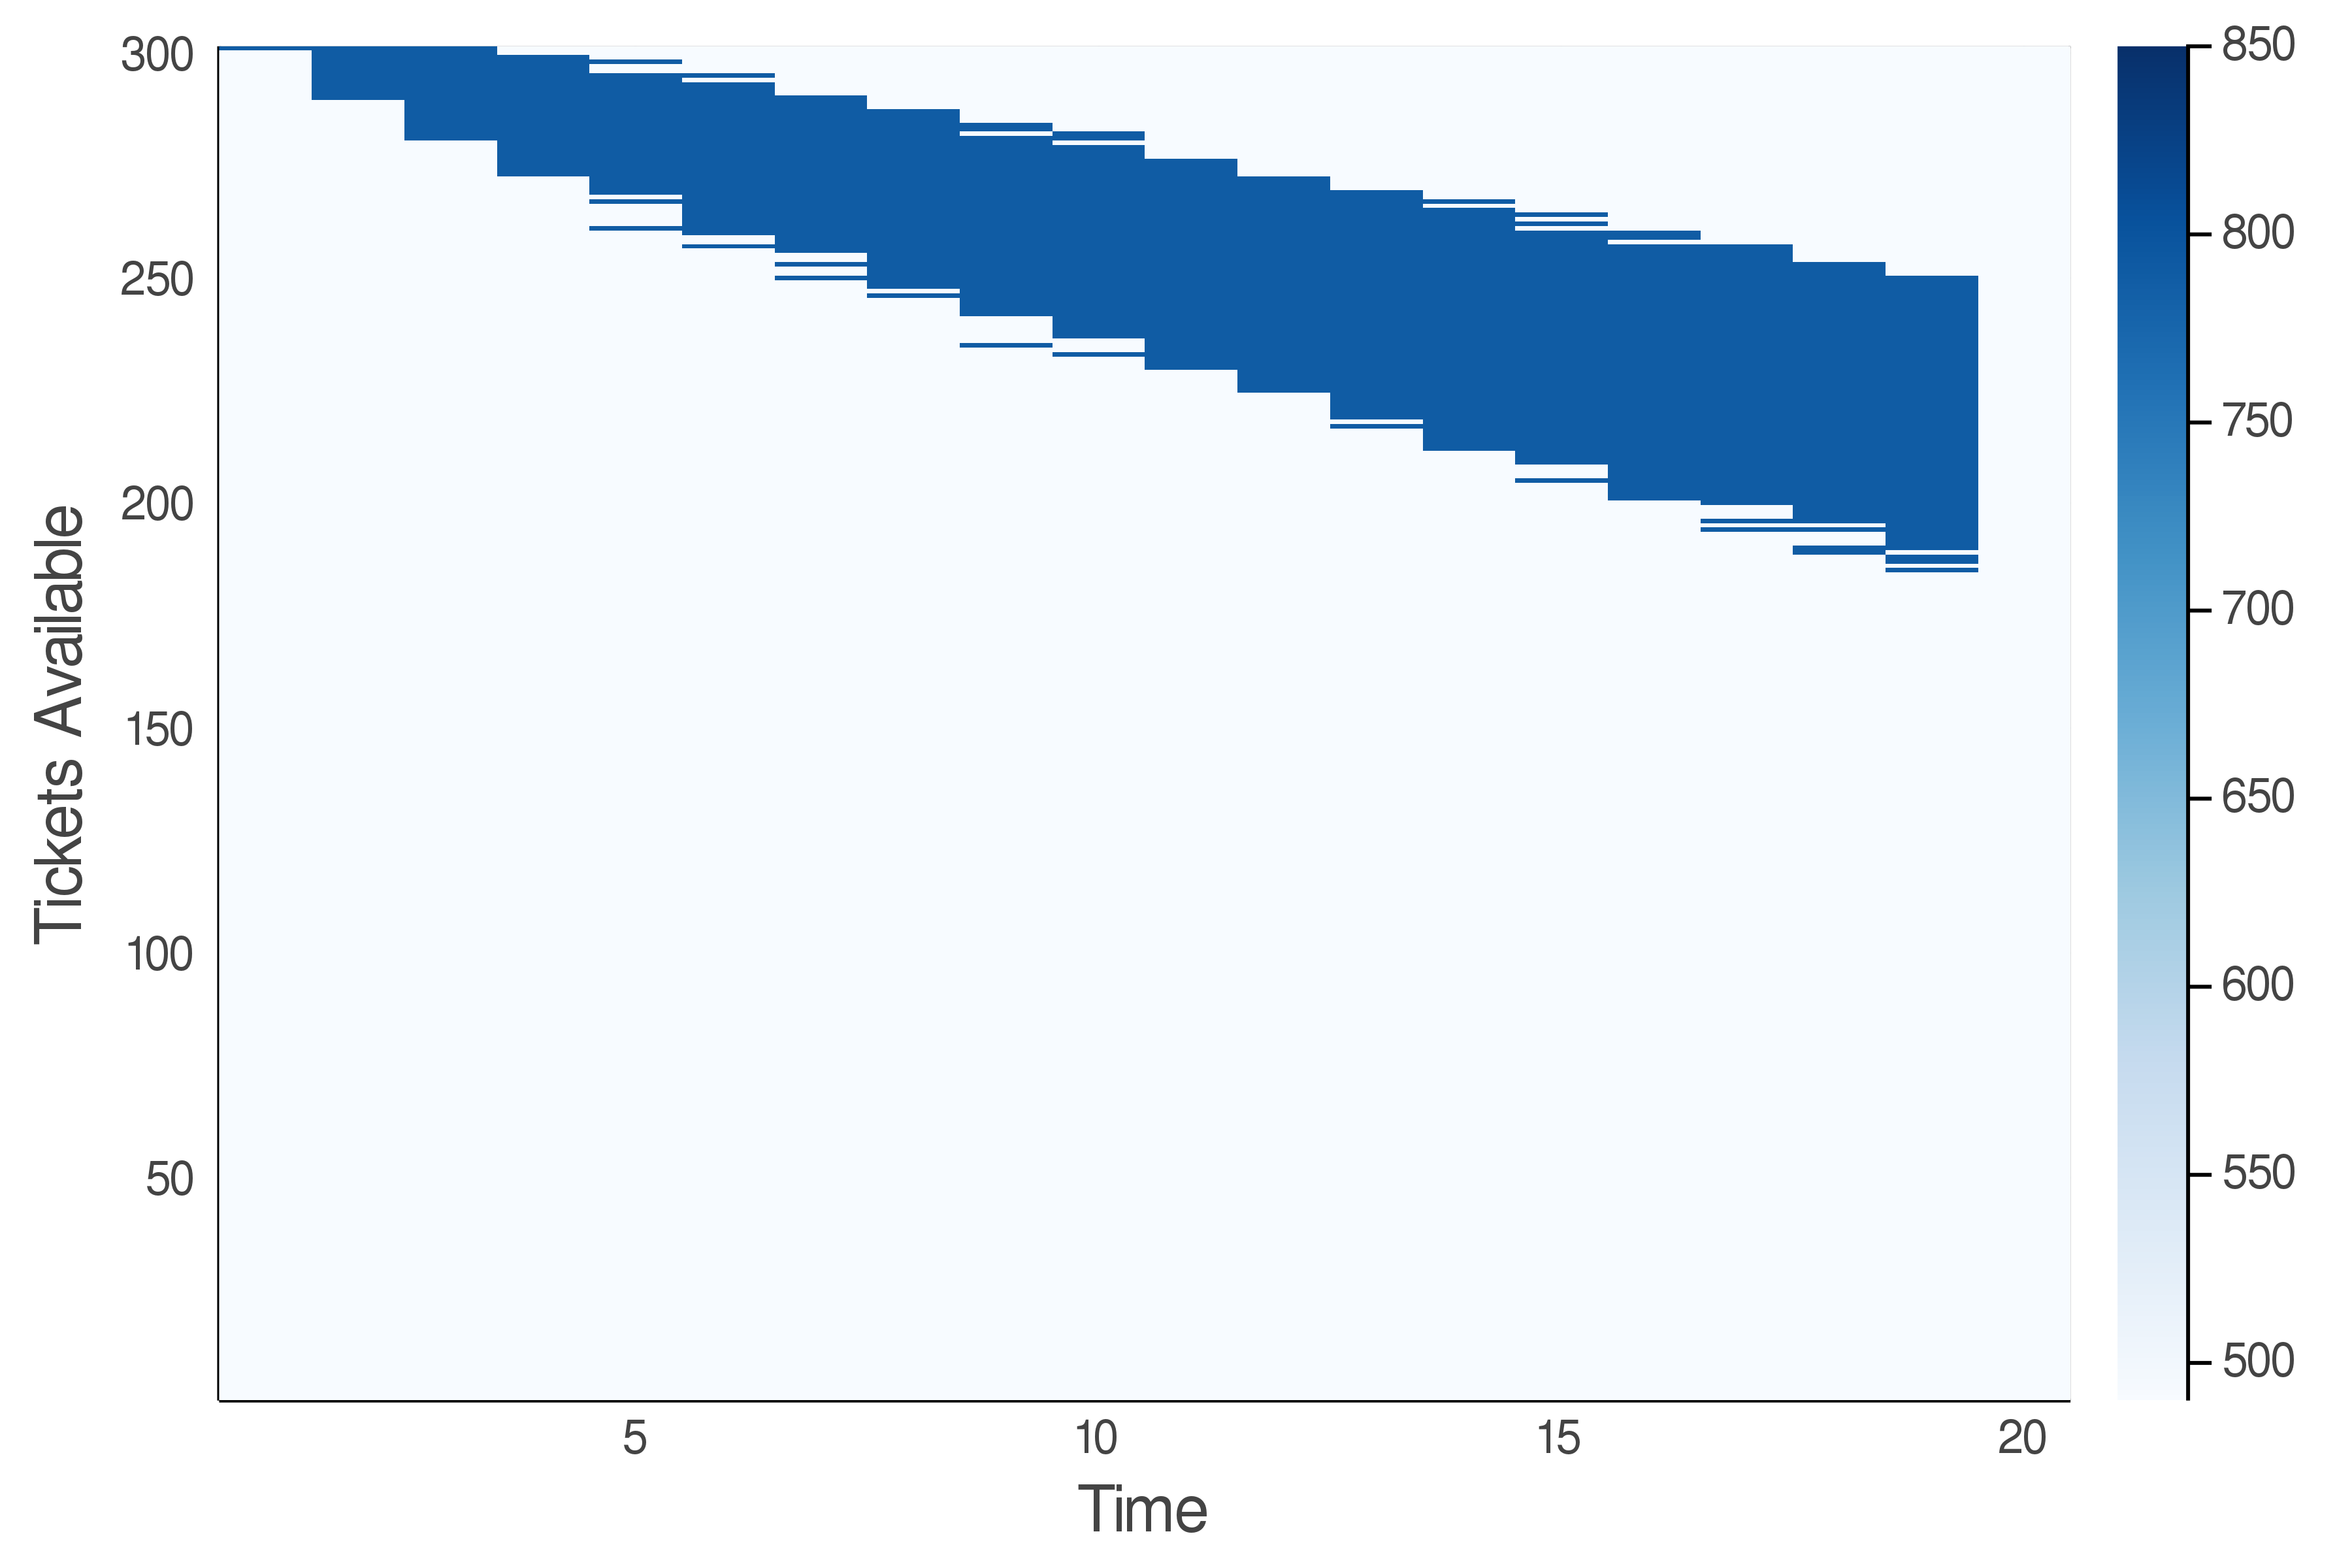
\includegraphics[width=0.3\linewidth]{final-paper/plots/singleAgentStaticHigh-policy.png}
    \caption{Optimal policies learned for the single fare class case (fare class 1) using the cheapest price (\textit{left}), a random policy (\textit{center}), and the most expensive price (\textit{right}).}
\end{figure}

\vfill\null

\begin{figure}[h!]
    \centering
    \label{fig:two-class-sarsa-U}
    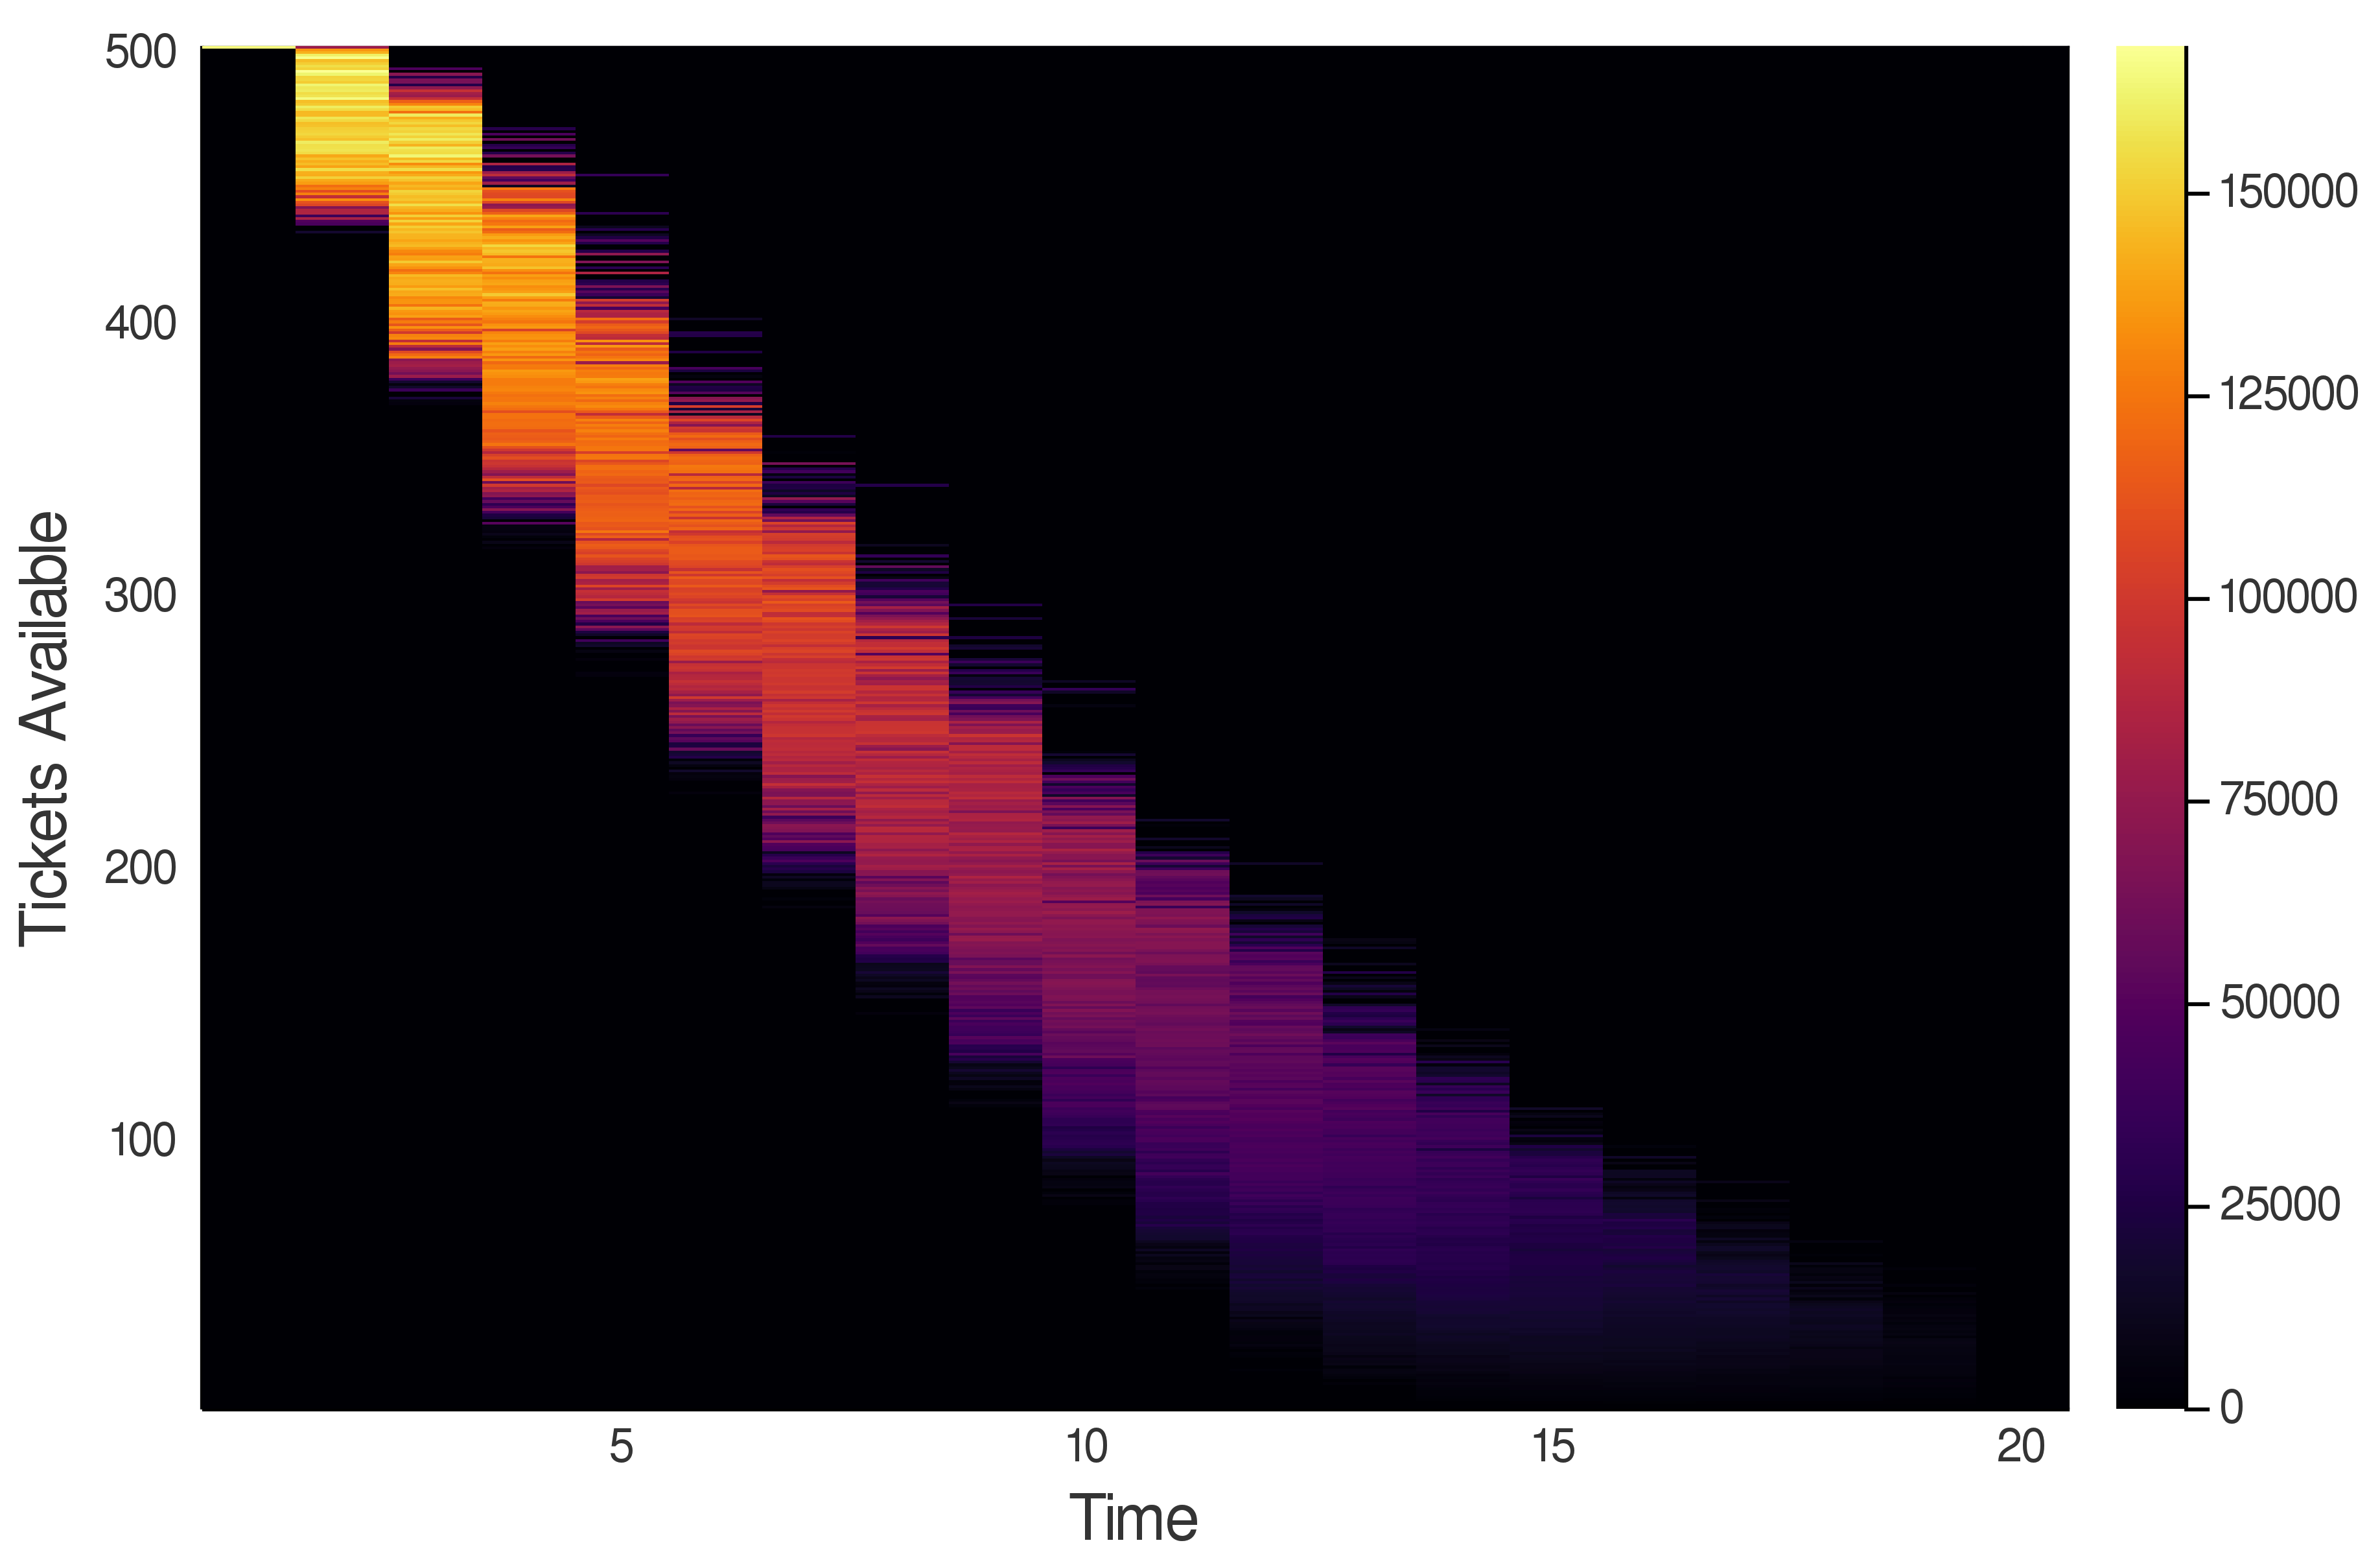
\includegraphics[width=0.48\linewidth]{final-paper/plots/doubleAgentSarsa-U.png} \;
    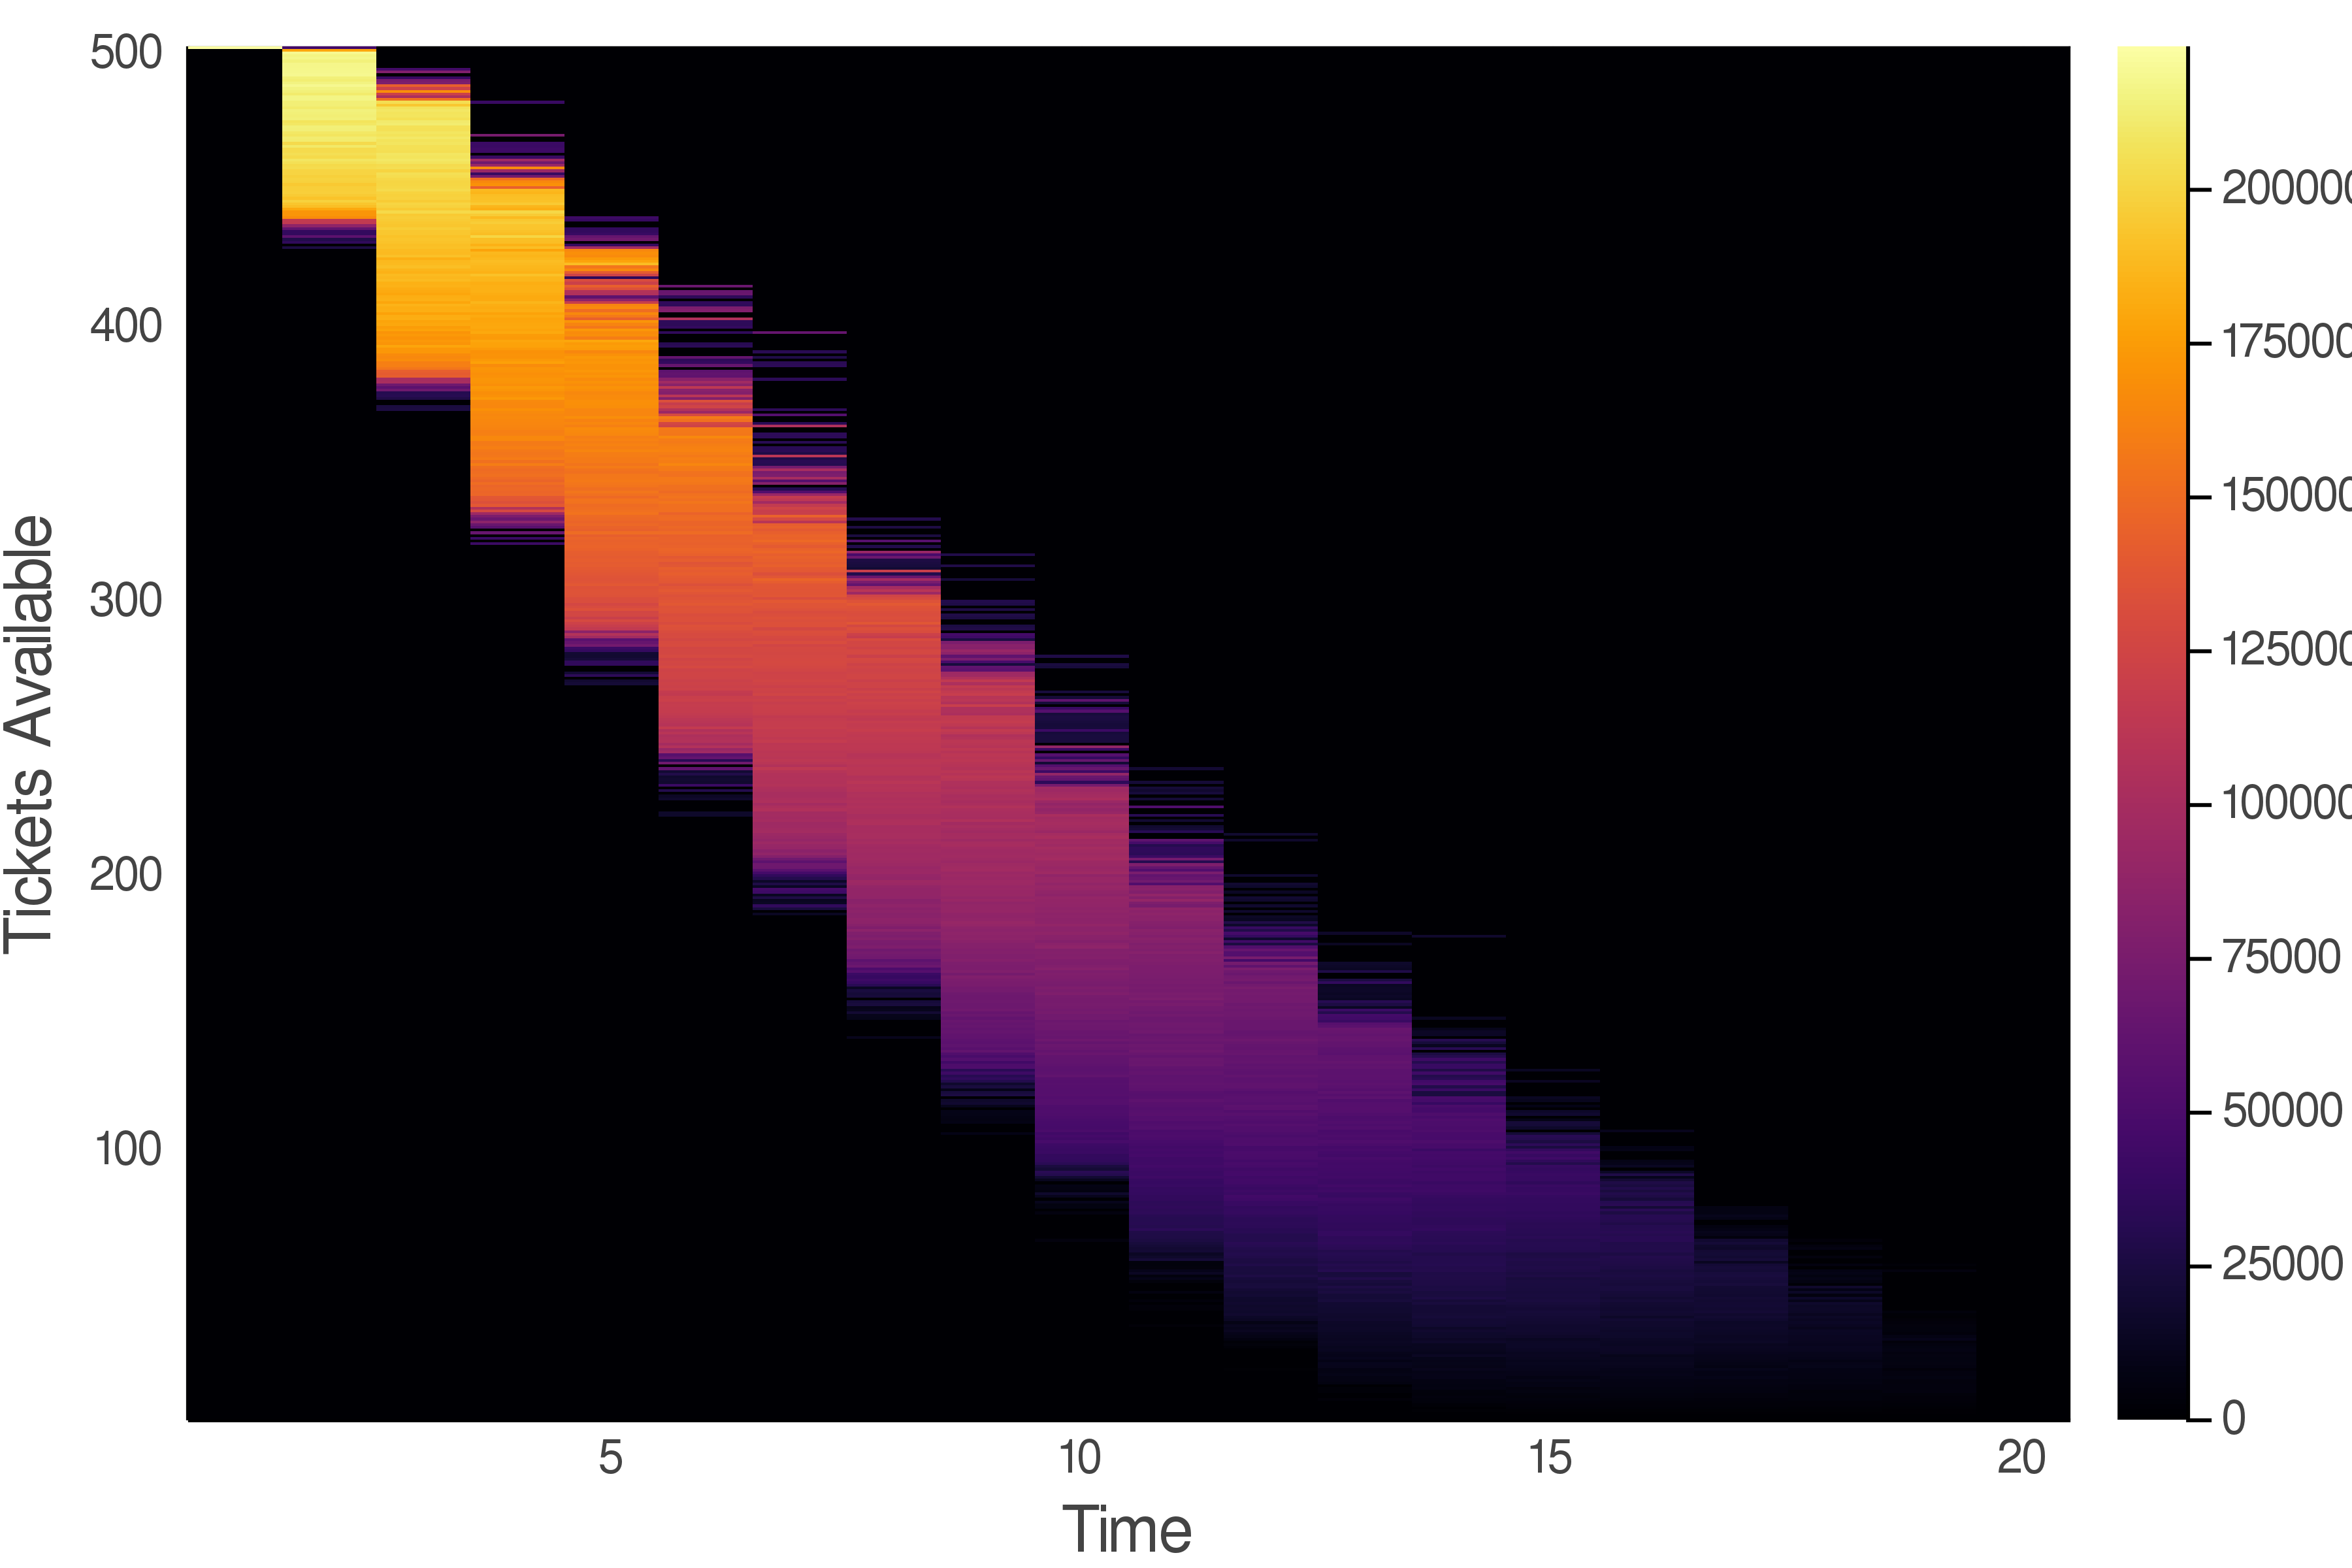
\includegraphics[width=0.48\linewidth]{final-paper/plots/doubleAgentSarsaLambda-U.png}
    \caption{Optimal value functions for the two fare class case trained using Sarsa (\textit{left}) and Sarsa($\lambda$) (\textit{right}).}
\end{figure}

\begin{figure}[h!]
    \centering
    \label{fig:two-class-sarsa-policy1}
    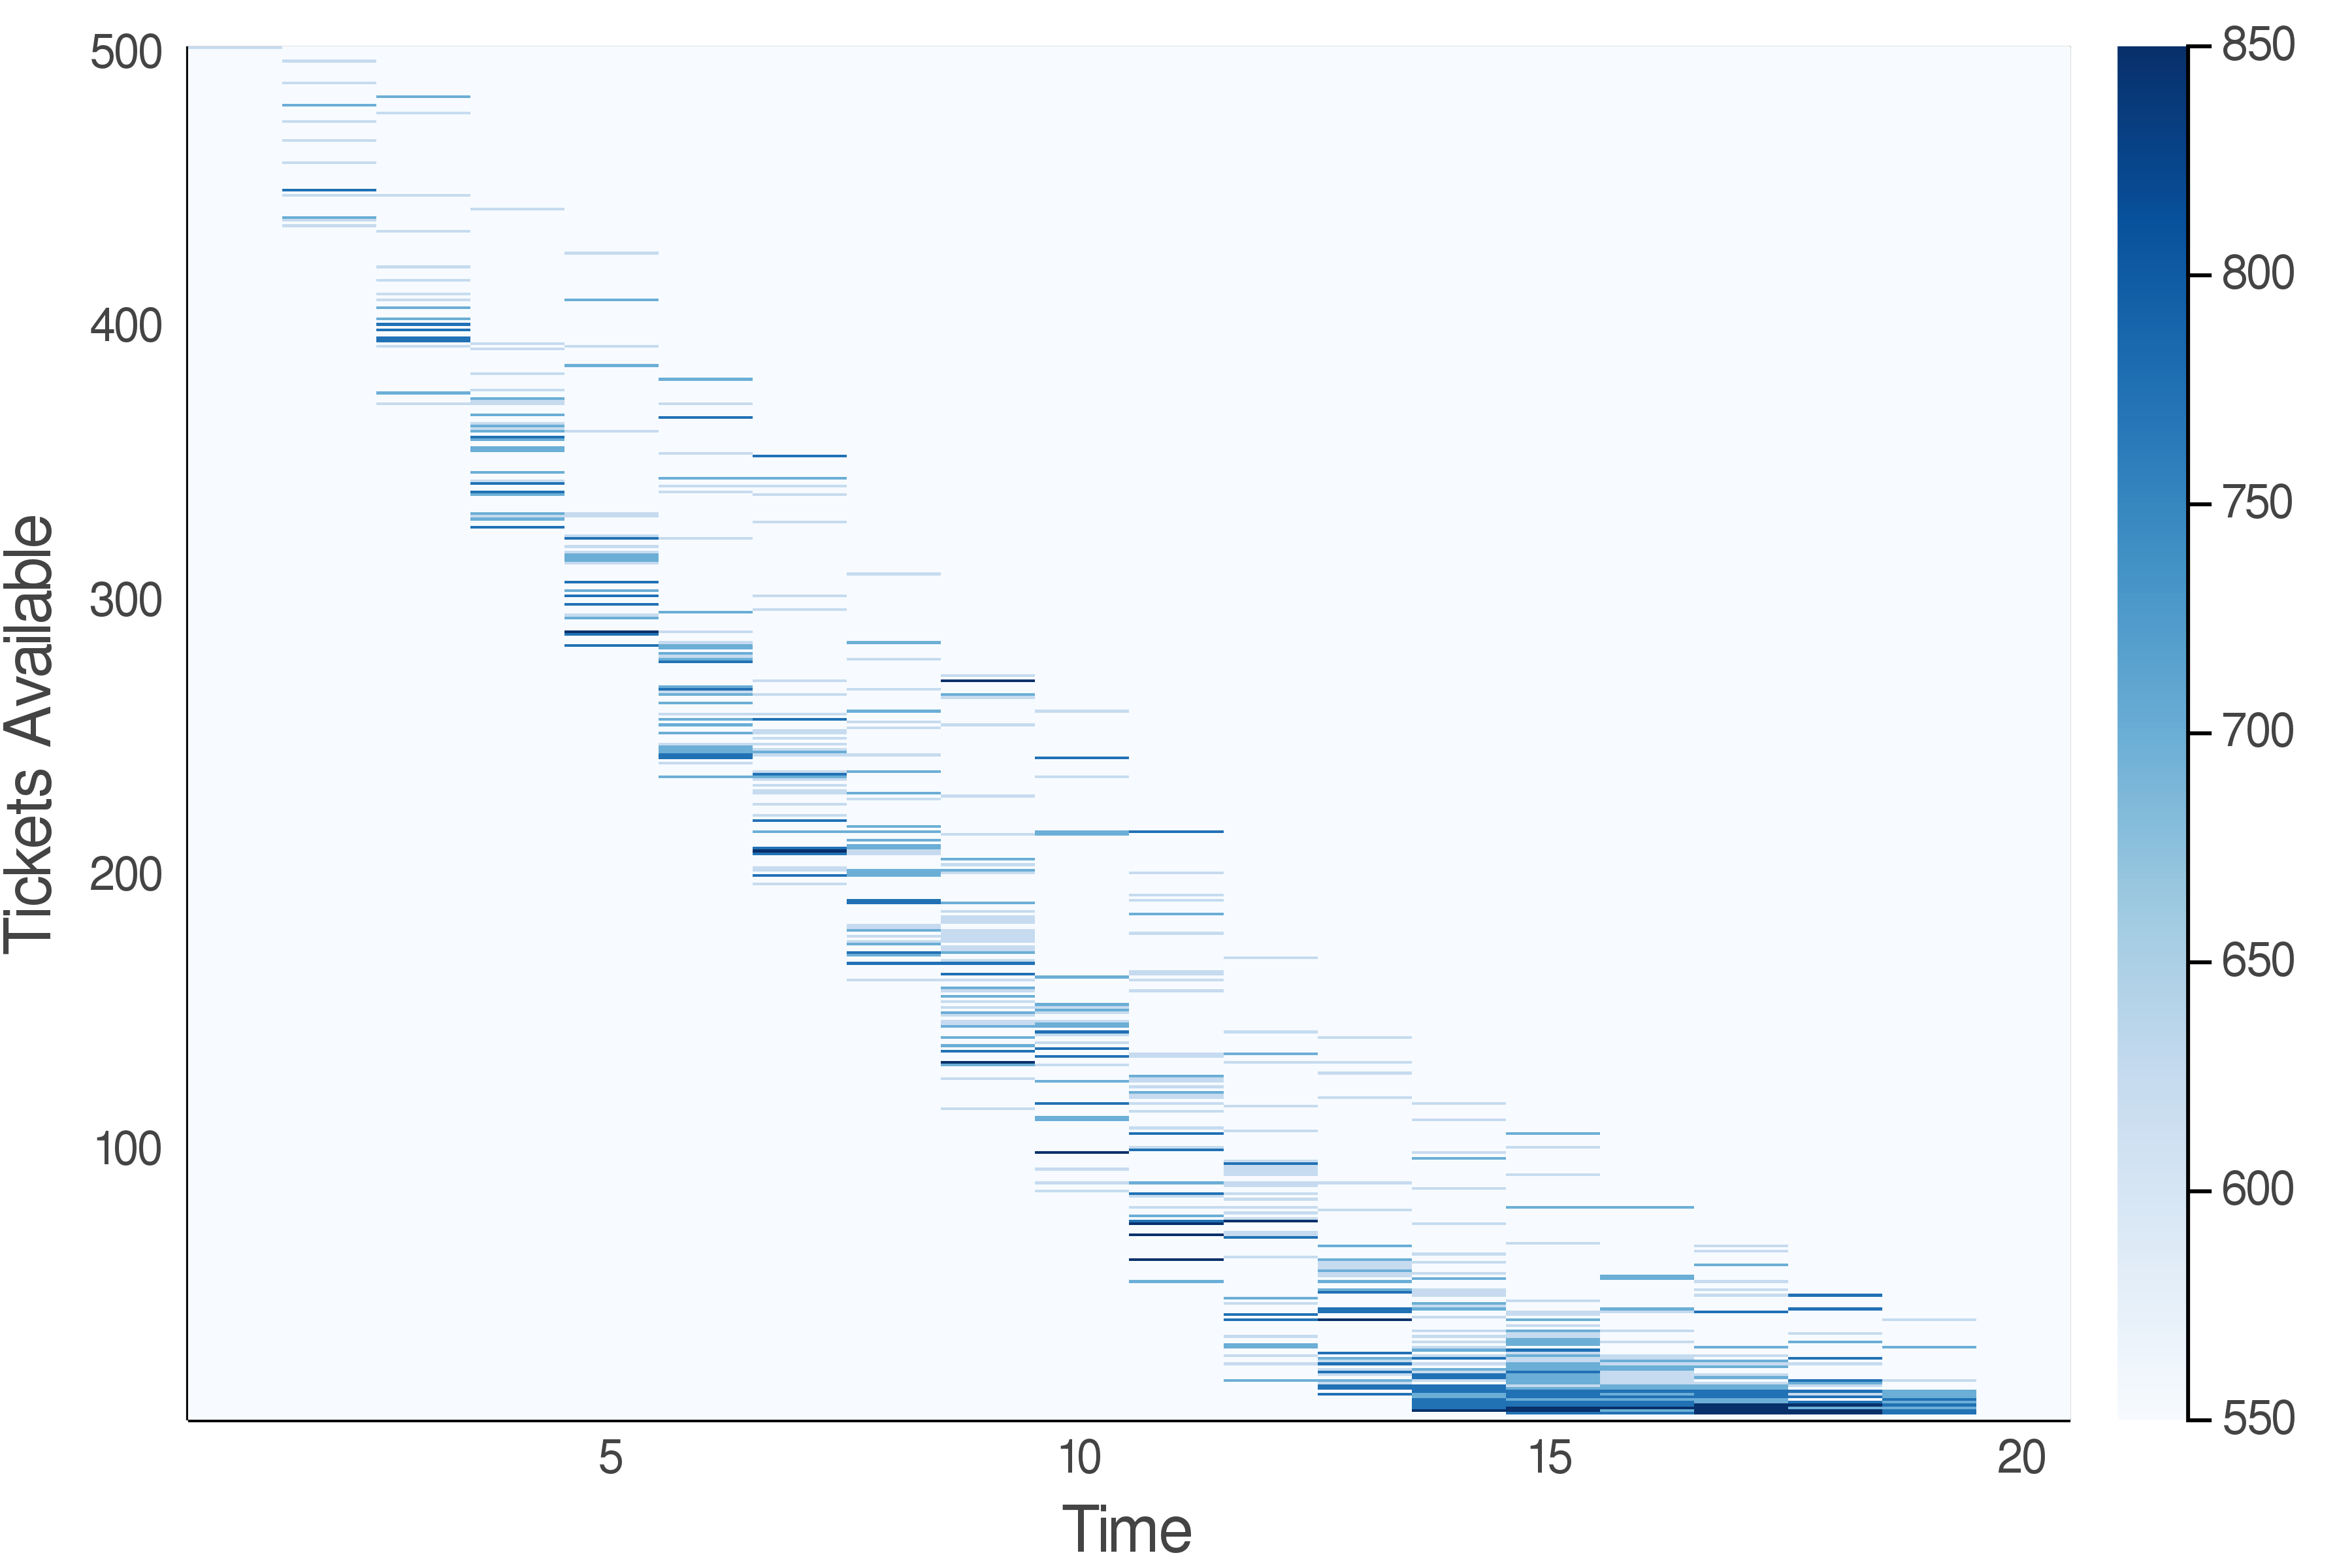
\includegraphics[width=0.48\linewidth]{final-paper/plots/doubleAgentSarsa-1policy.png} \;
    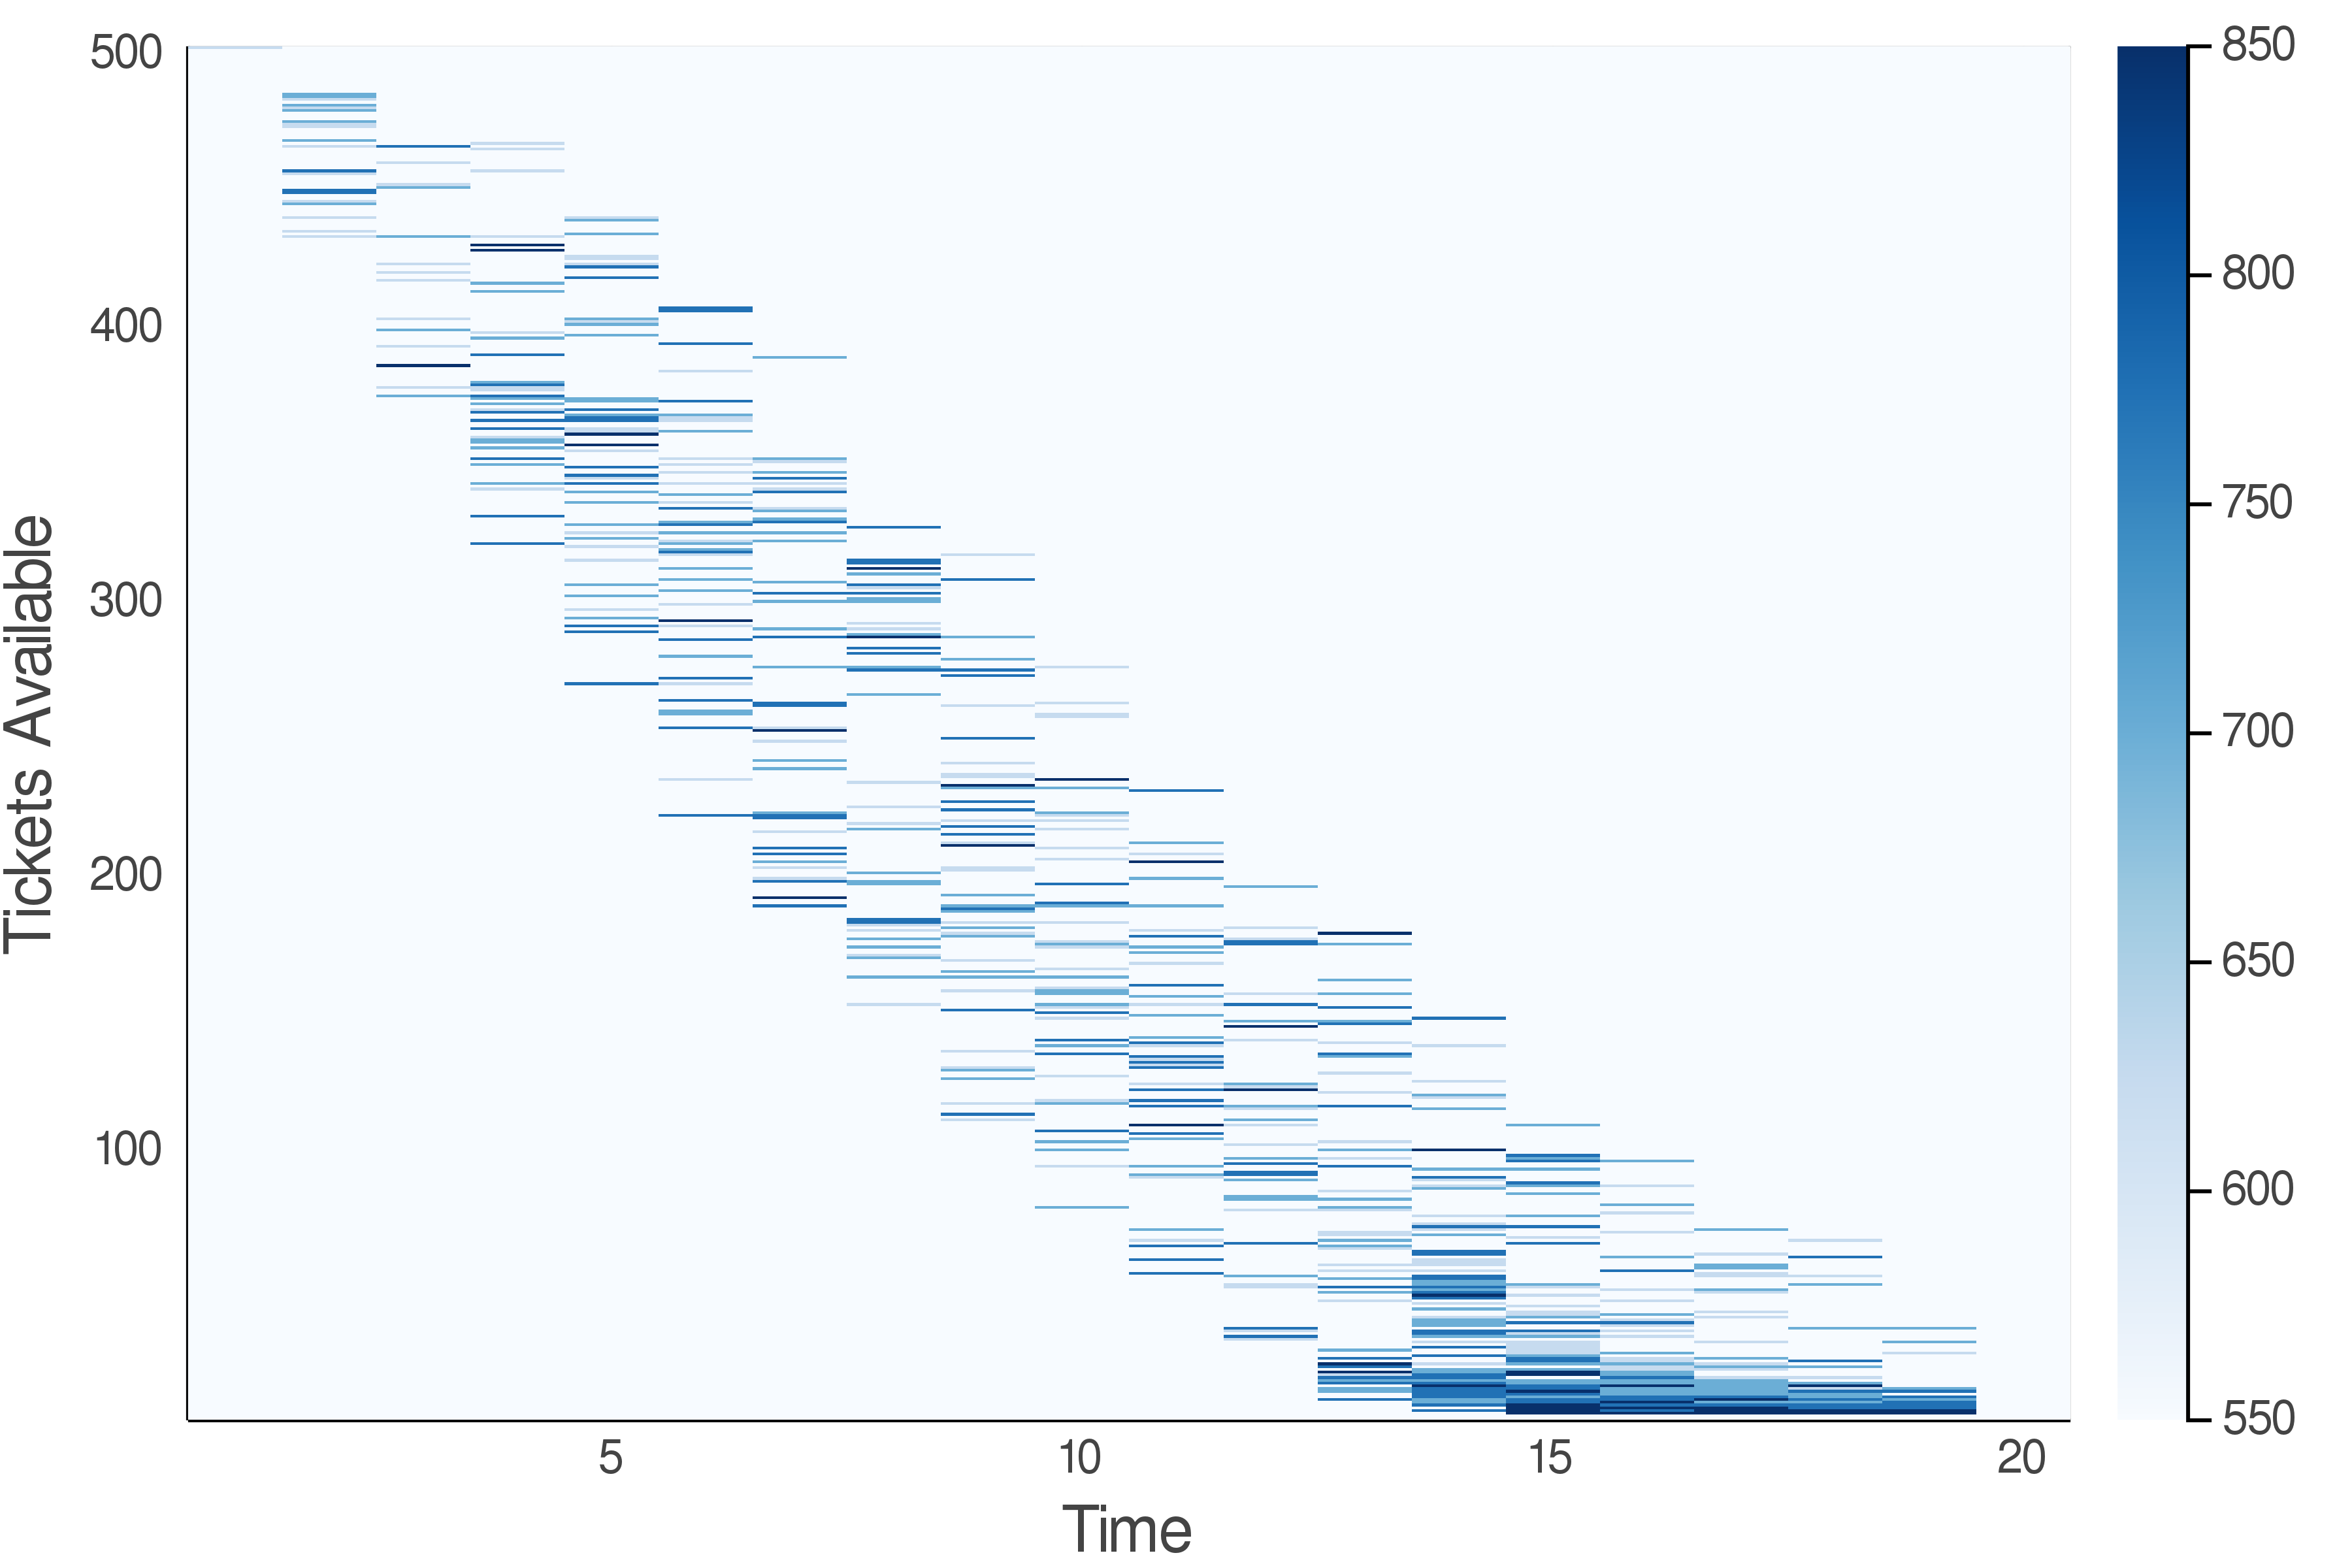
\includegraphics[width=0.48\linewidth]{final-paper/plots/doubleAgentSarsaLambda-1policy.png}
    \caption{Optimal pricing policies for the first fare class in dollars (\$) for the two fare class case trained using Sarsa (\textit{left}) and Sarsa($\lambda$) (\textit{right}).}
\end{figure}

\begin{figure}[h!]
    \centering
    \label{fig:two-class-sarsa-policy2}
    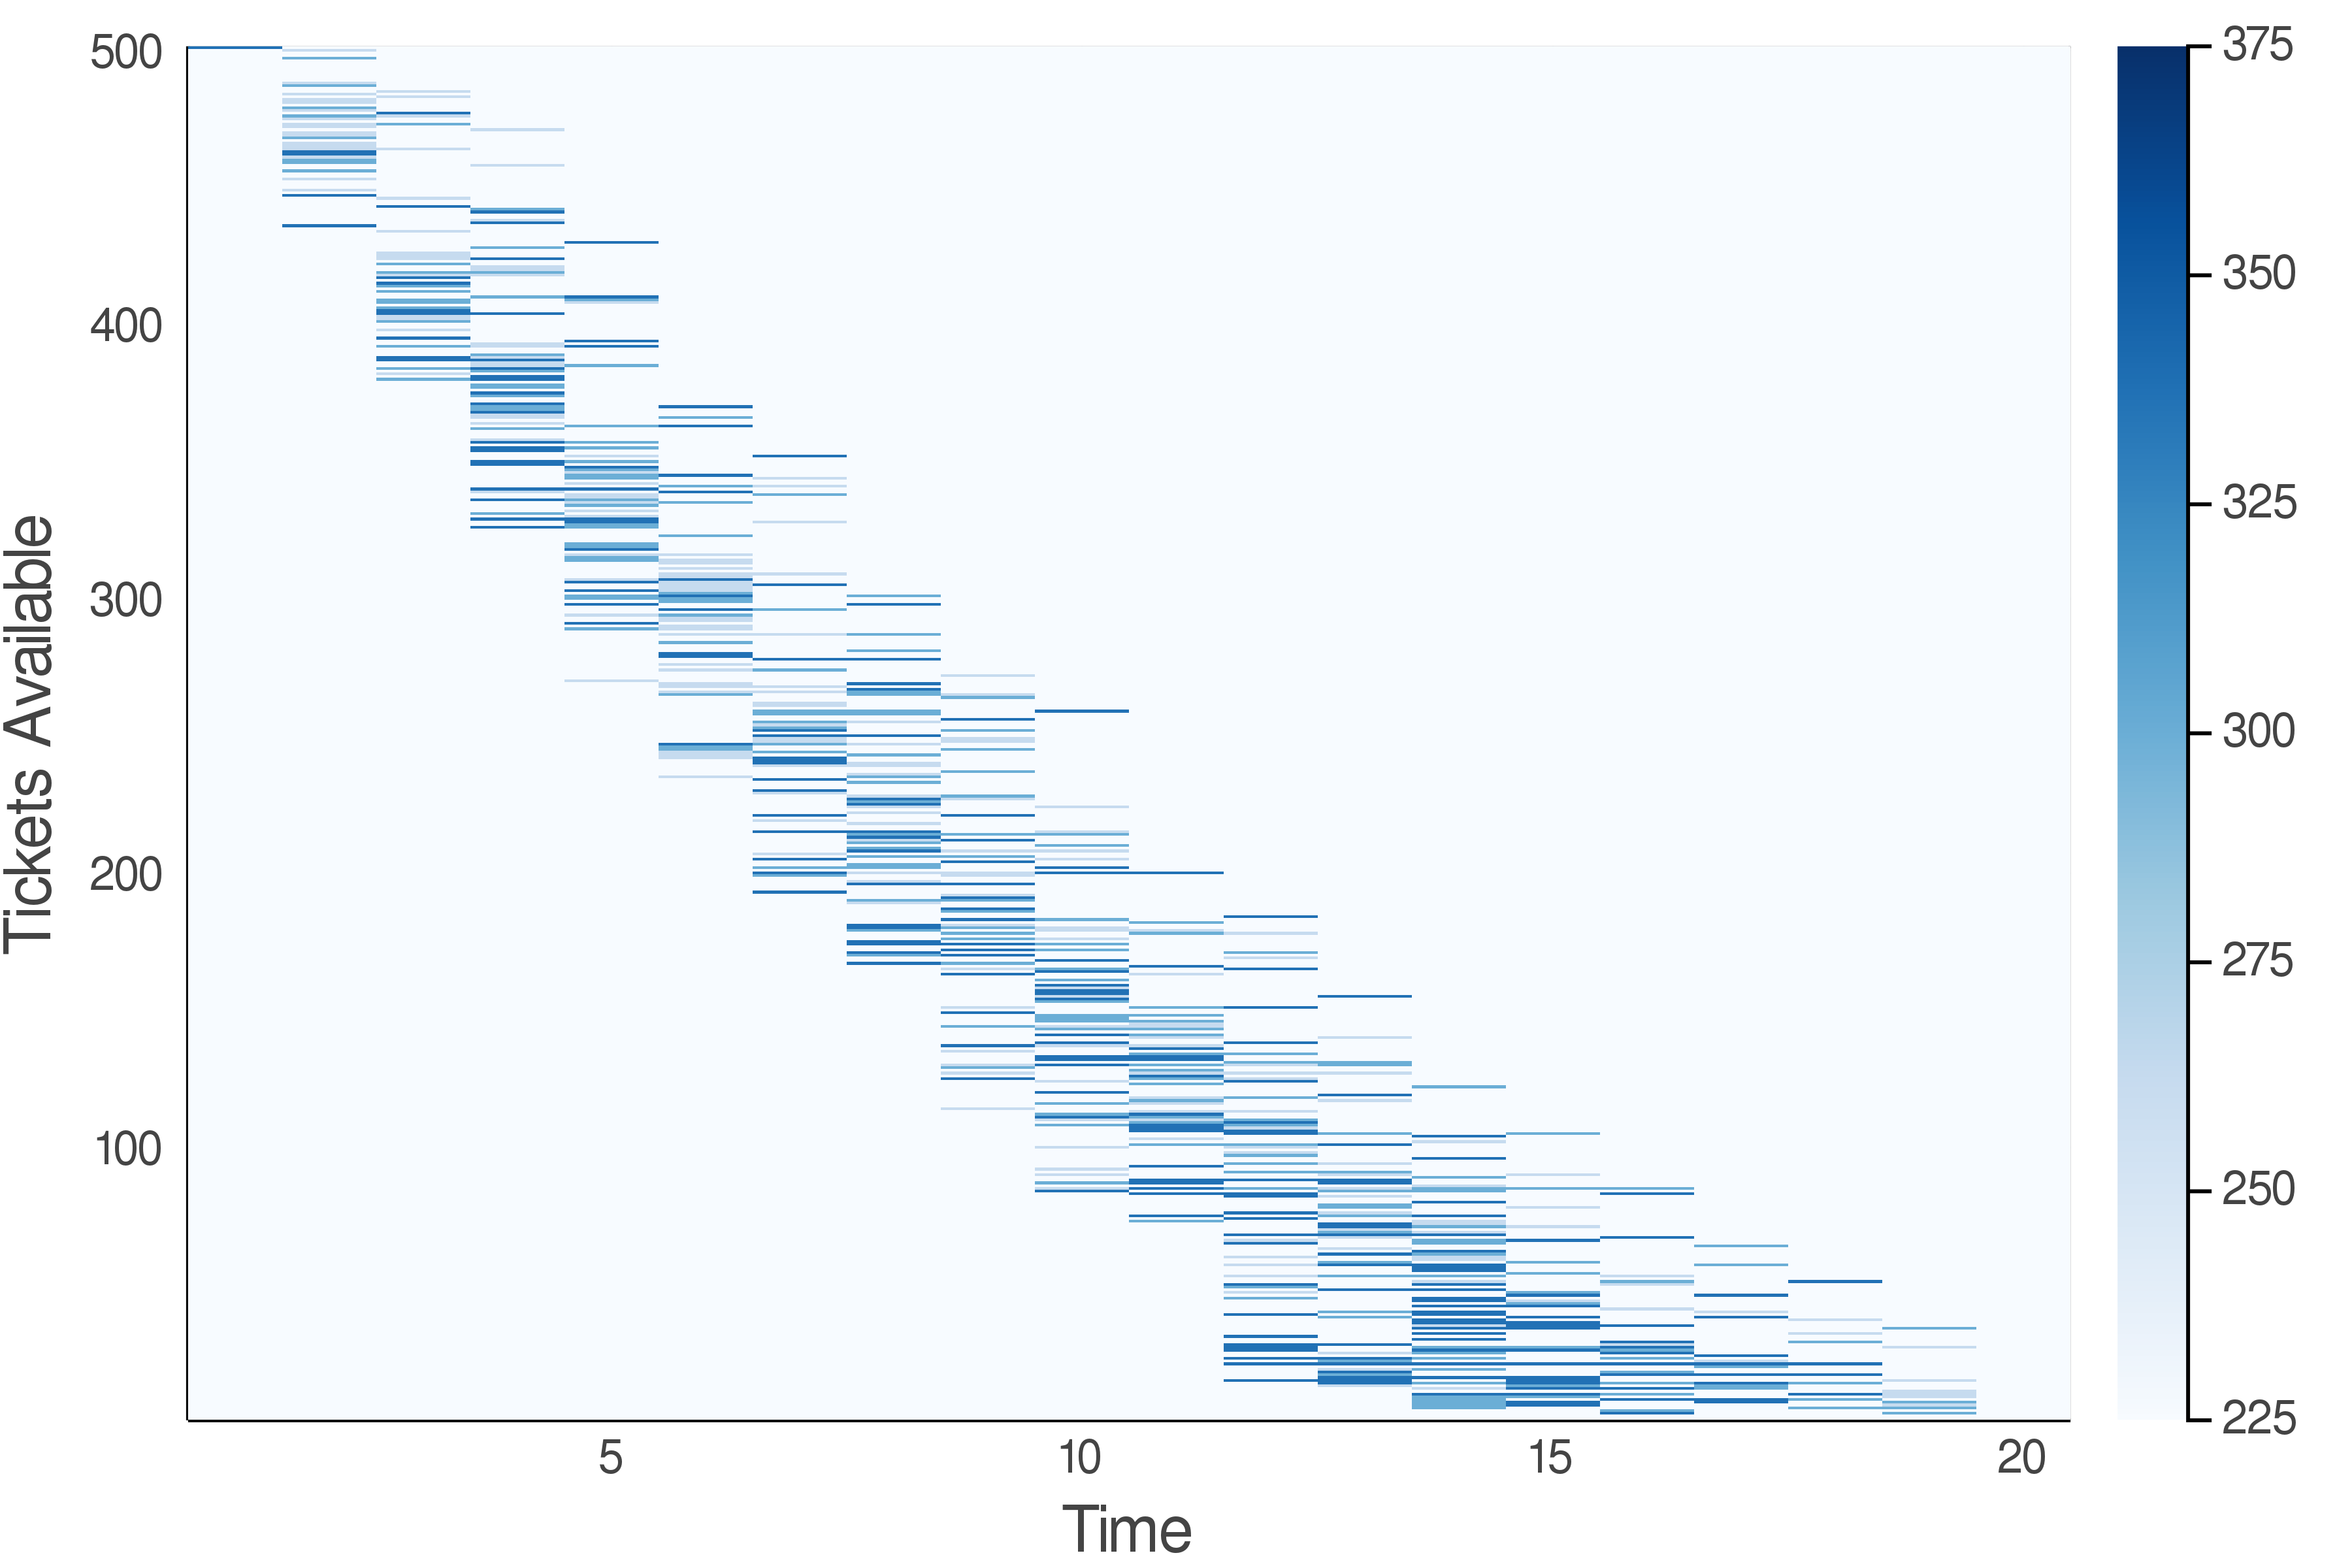
\includegraphics[width=0.48\linewidth]{final-paper/plots/doubleAgentSarsa-2policy.png} \;
    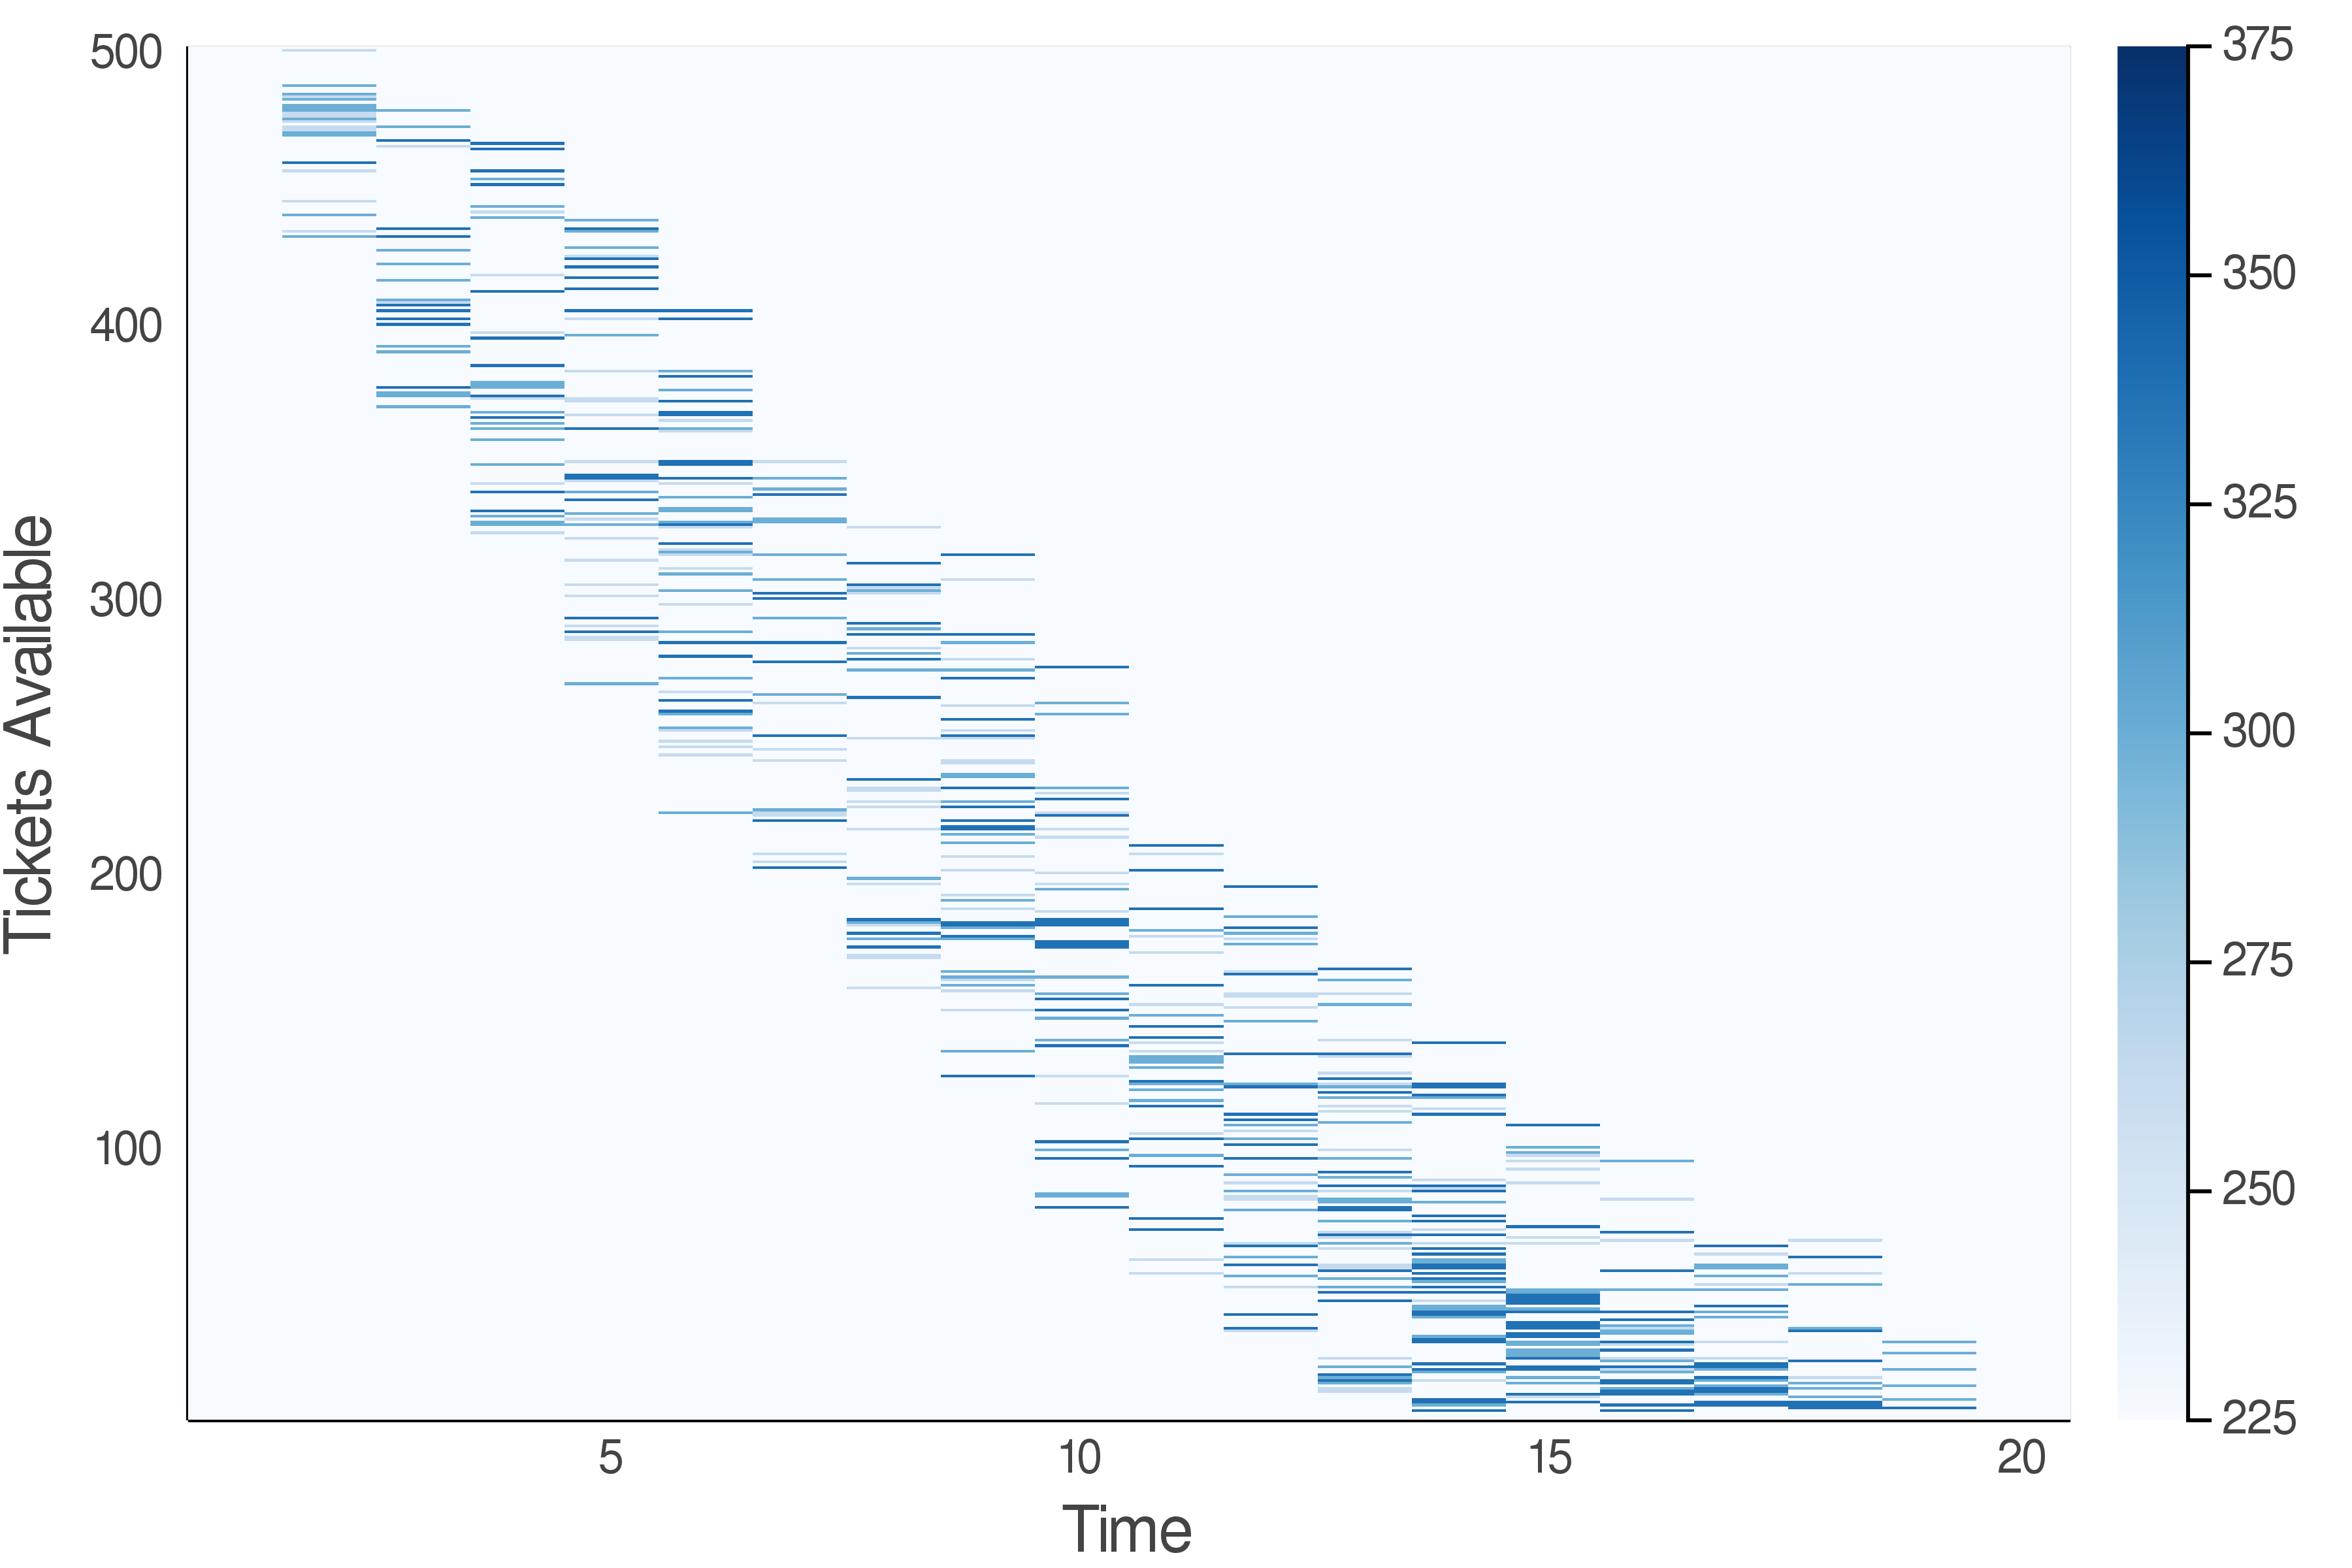
\includegraphics[width=0.48\linewidth]{final-paper/plots/doubleAgentSarsaLambda-2policy.png}
    \caption{Optimal pricing policies for the second fare class in dollars (\$) for the two fare class case trained using Sarsa (\textit{left}) and Sarsa($\lambda$) (\textit{right}).}
\end{figure}

\begin{figure}[h!]
    \centering
    \label{fig:two-class-baselines-U}
    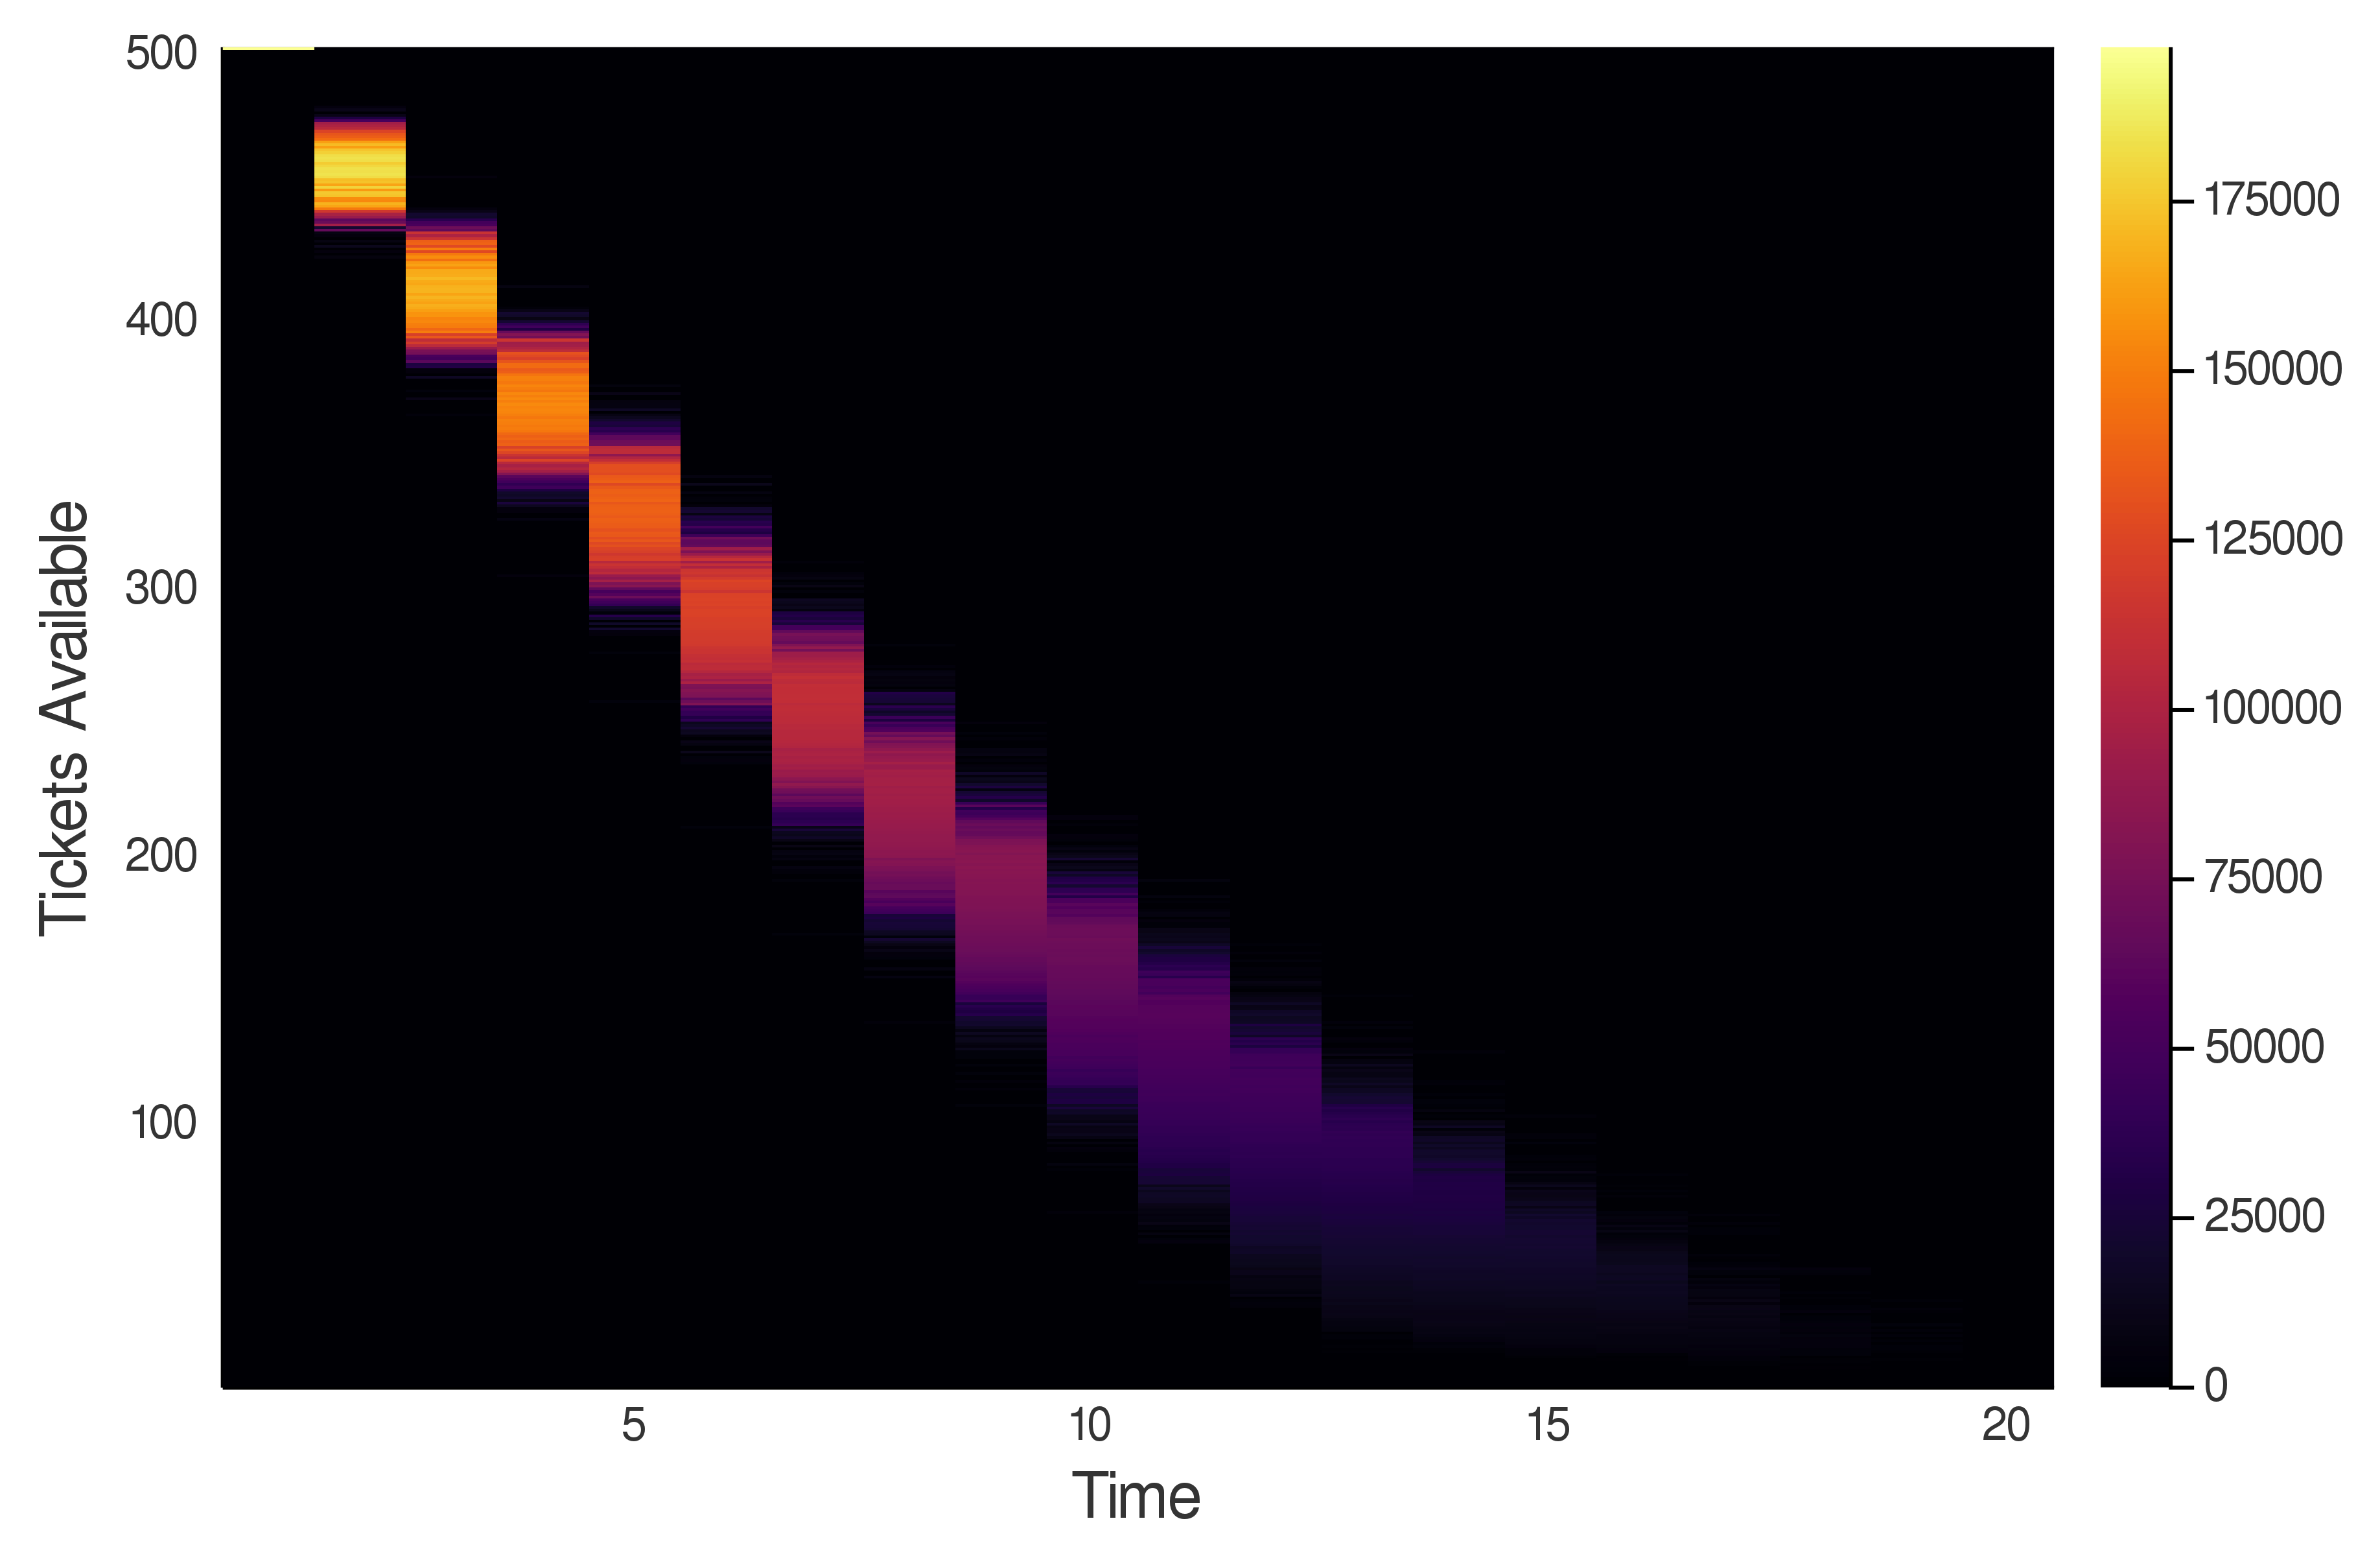
\includegraphics[width=0.3\linewidth]{final-paper/plots/doubleAgentStaticLow-U.png} \;
    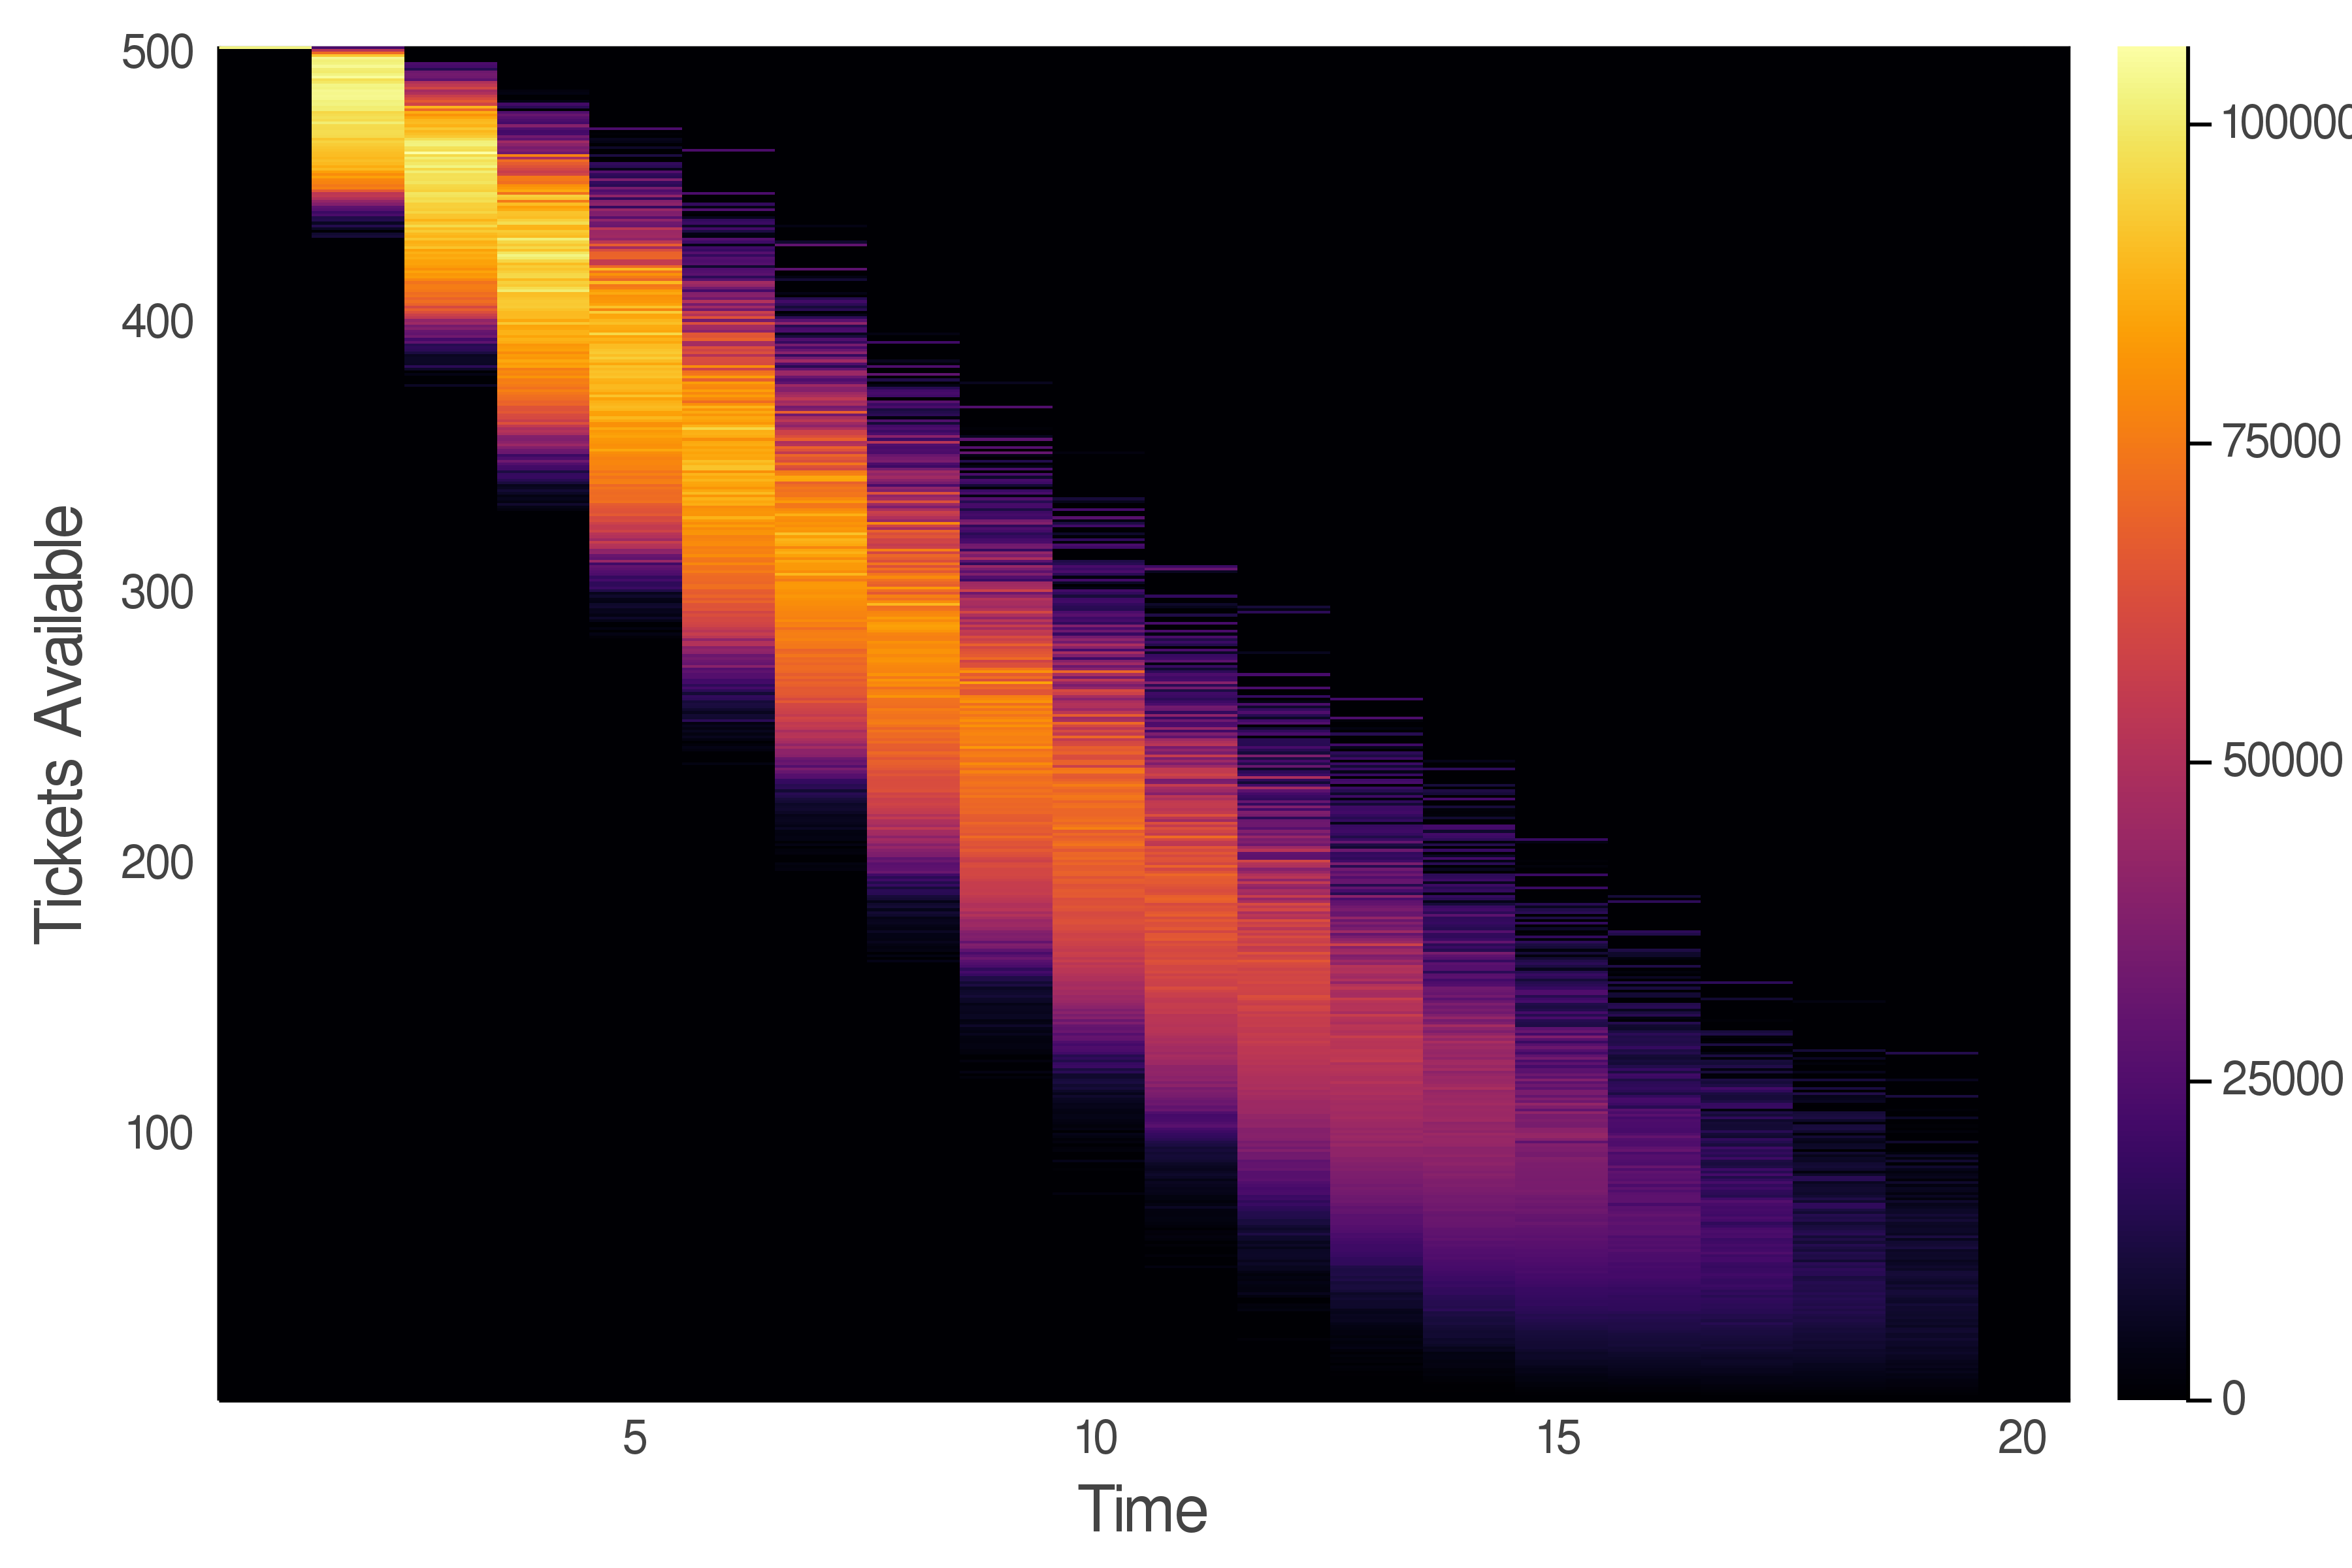
\includegraphics[width=0.3\linewidth]{final-paper/plots/doubleAgentRandom-U.png} \;
    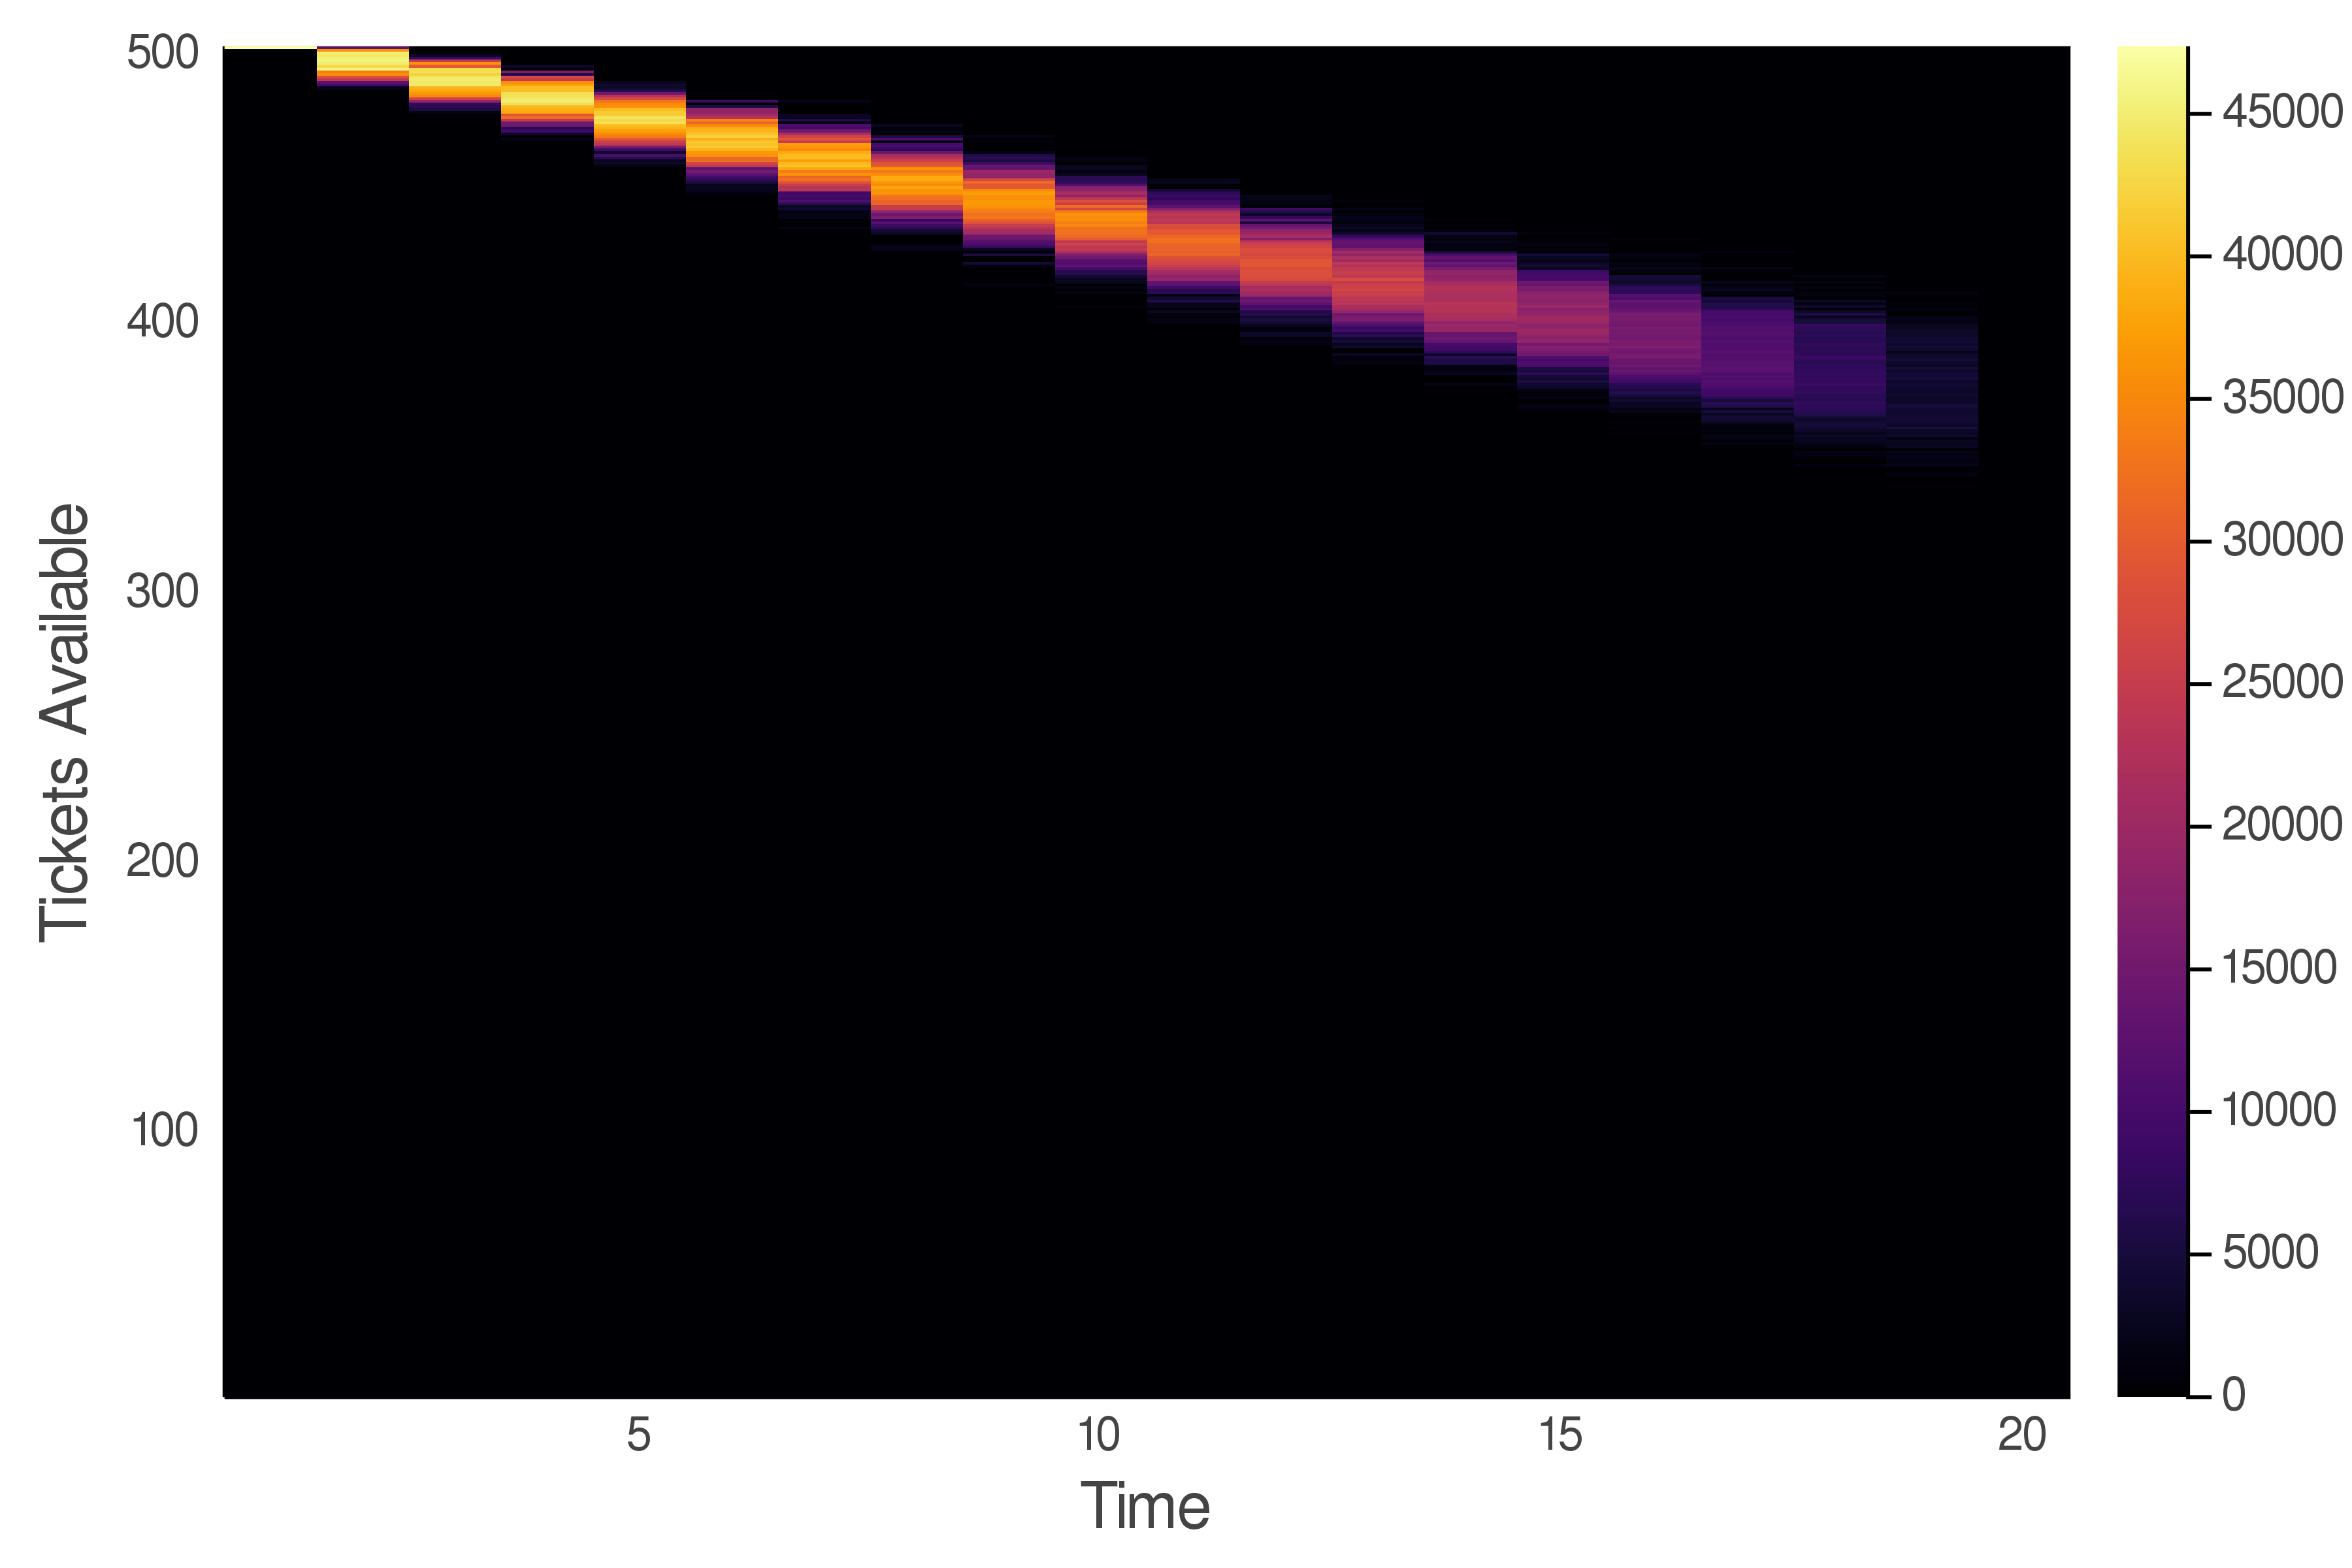
\includegraphics[width=0.3\linewidth]{final-paper/plots/doubleAgentStaticHigh-U.png}
    \caption{Optimal value functions for the two fare class case using the cheapest price (\textit{left}), a random policy (\textit{center}), and the most expensive price (\textit{right}).}
\end{figure}

\begin{figure}[h!]
    \centering
    \label{fig:two-class-baselines-policy1}
    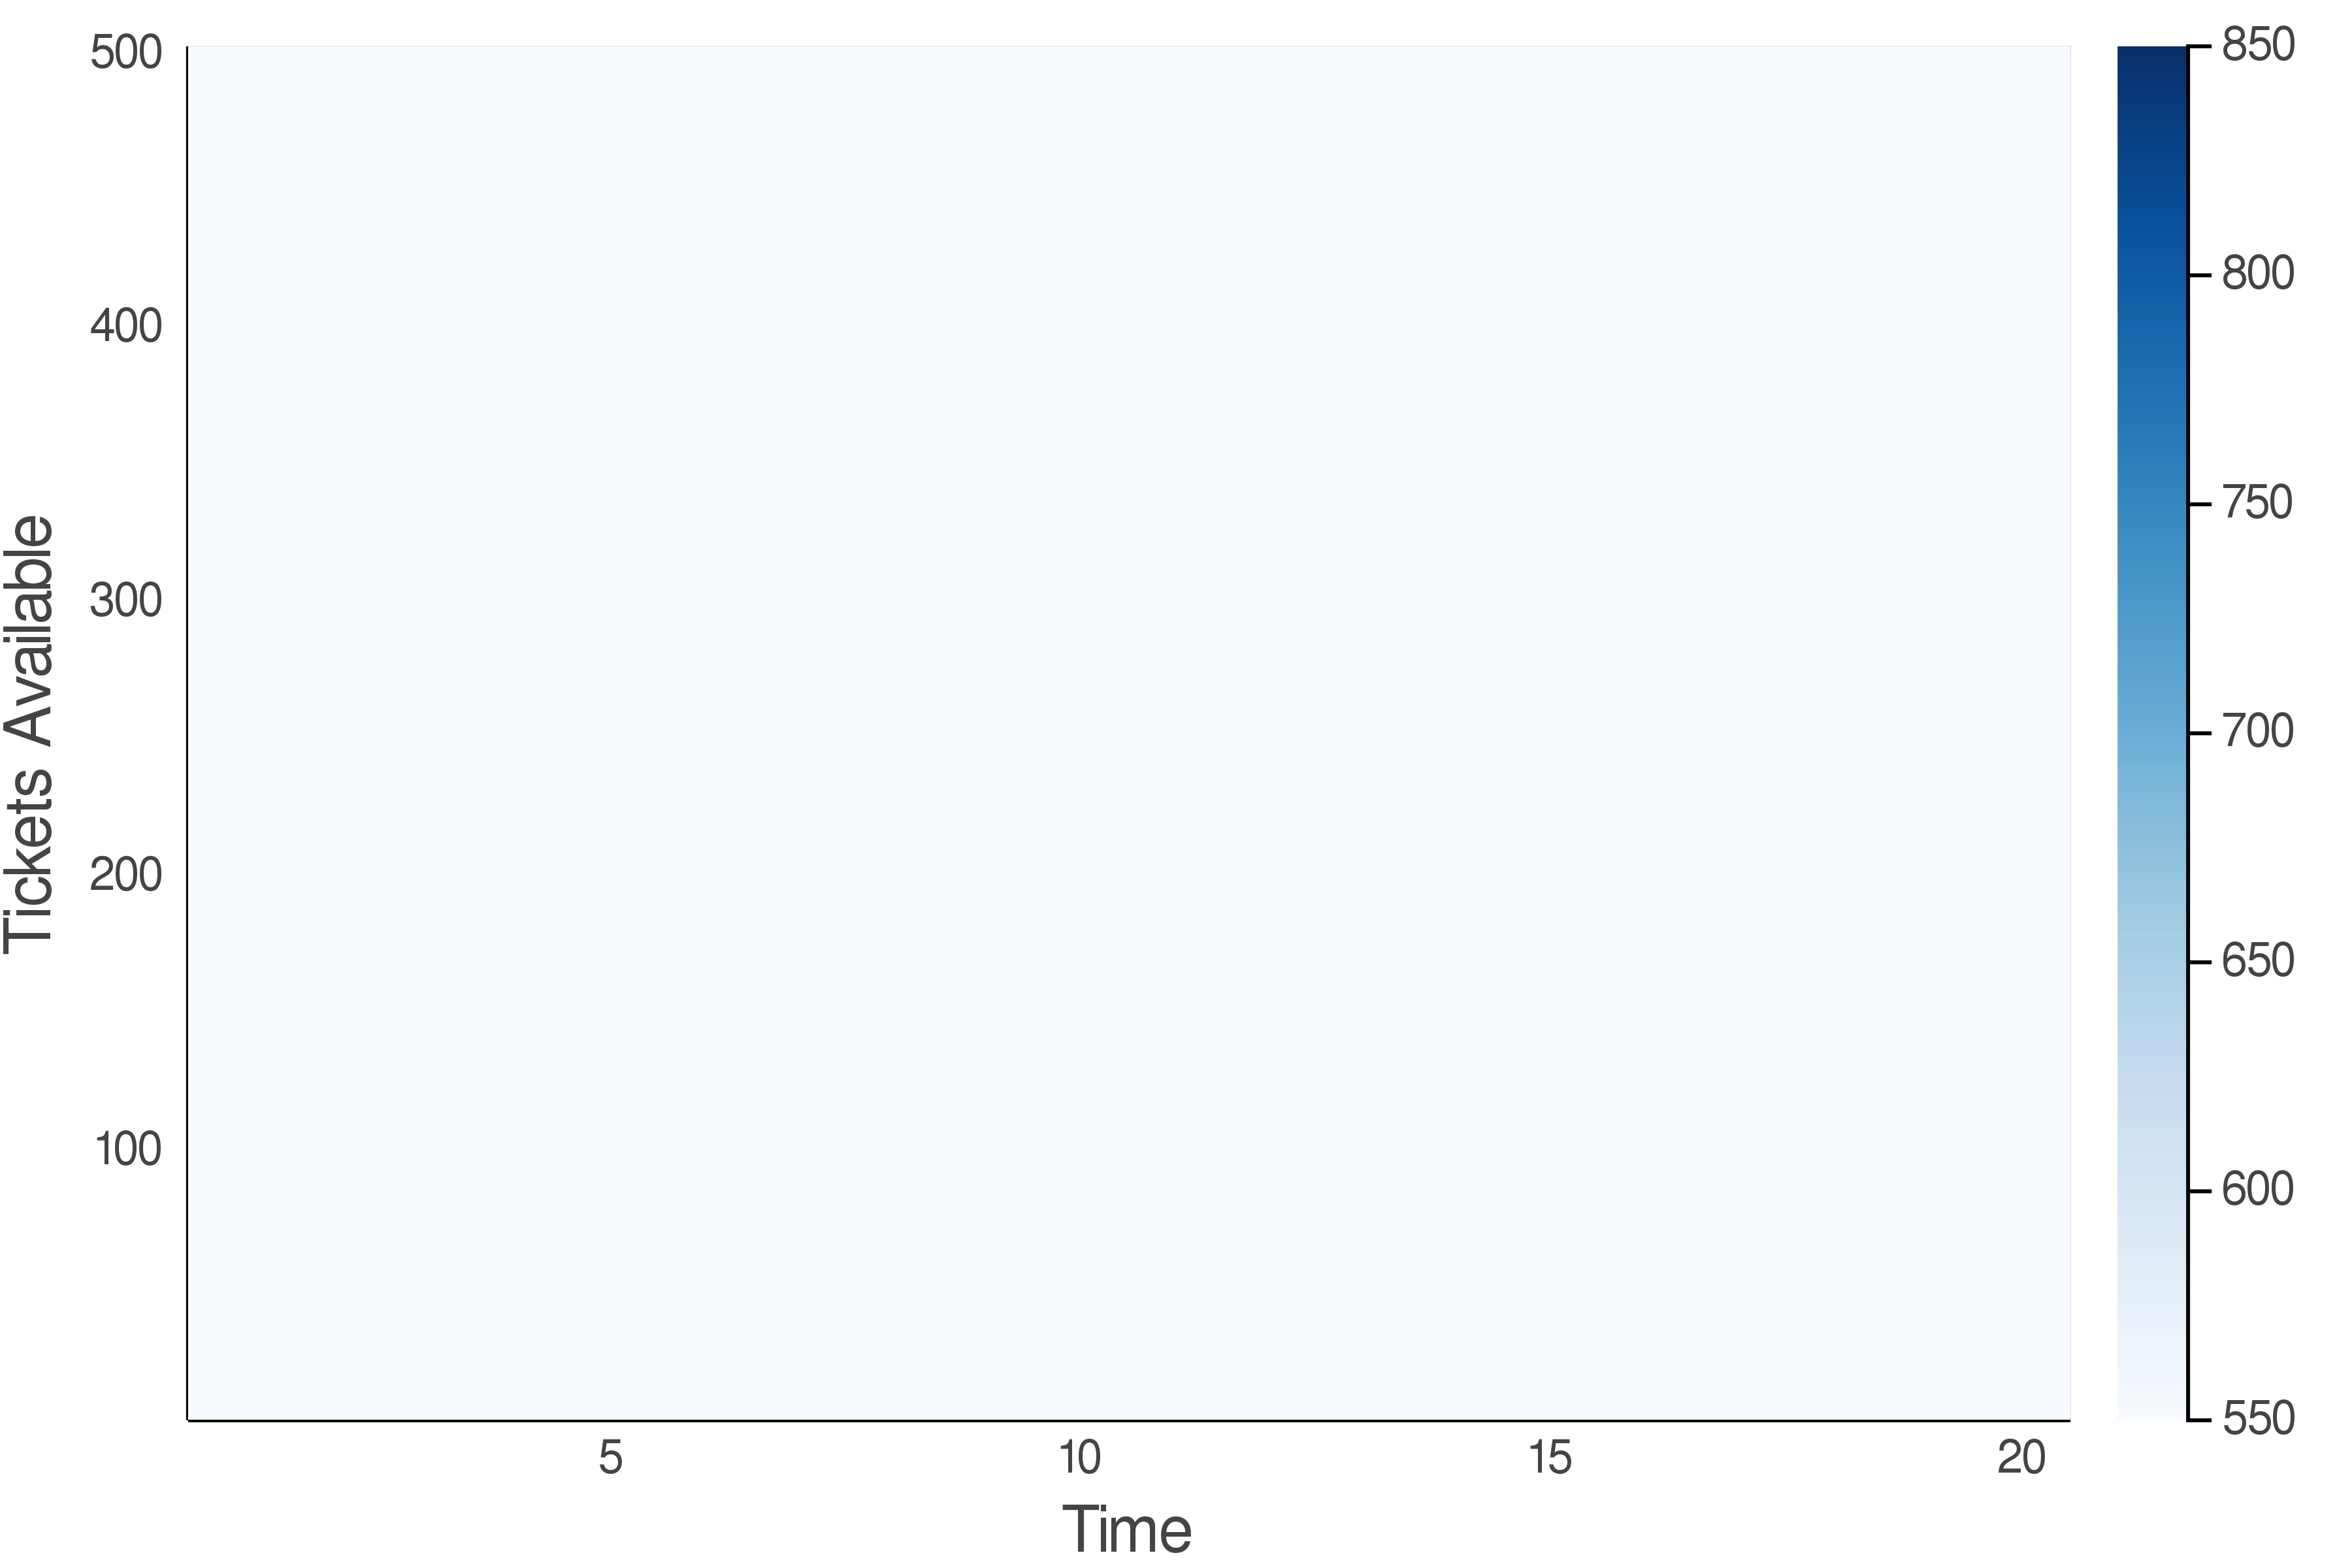
\includegraphics[width=0.3\linewidth]{final-paper/plots/doubleAgentStaticLow-1policy.png} \;
    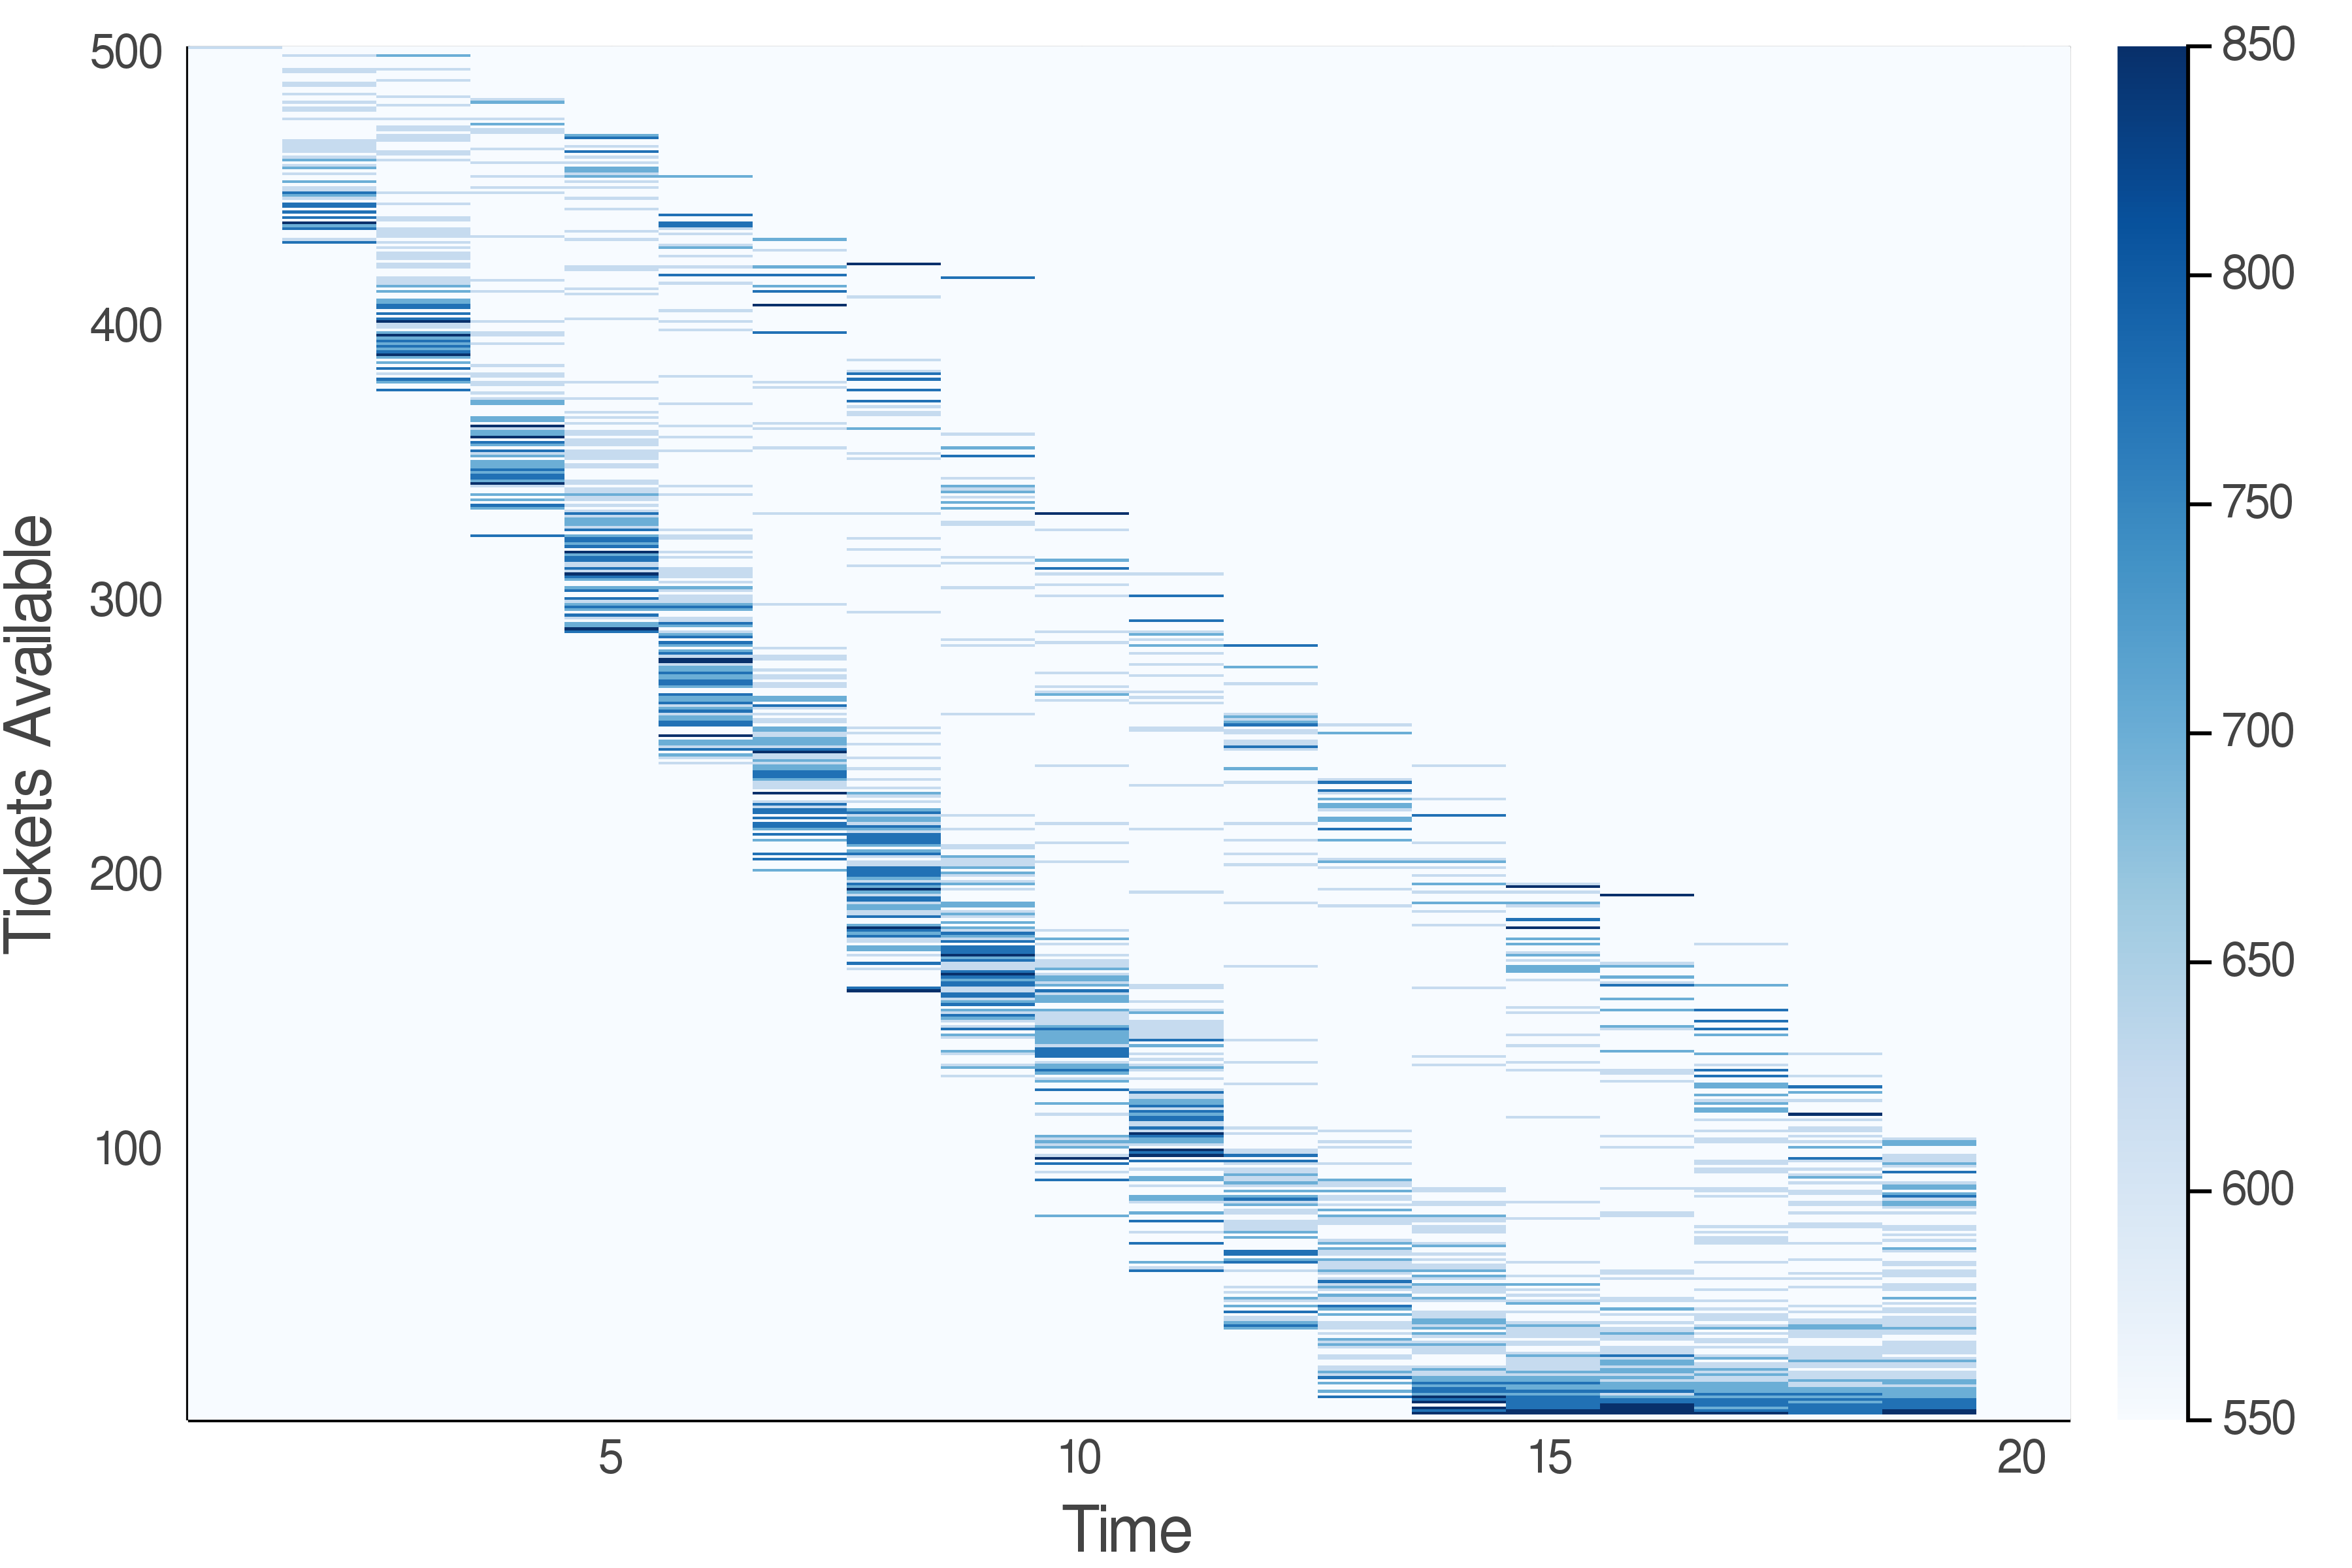
\includegraphics[width=0.3\linewidth]{final-paper/plots/doubleAgentRandom-1policy.png} \;
    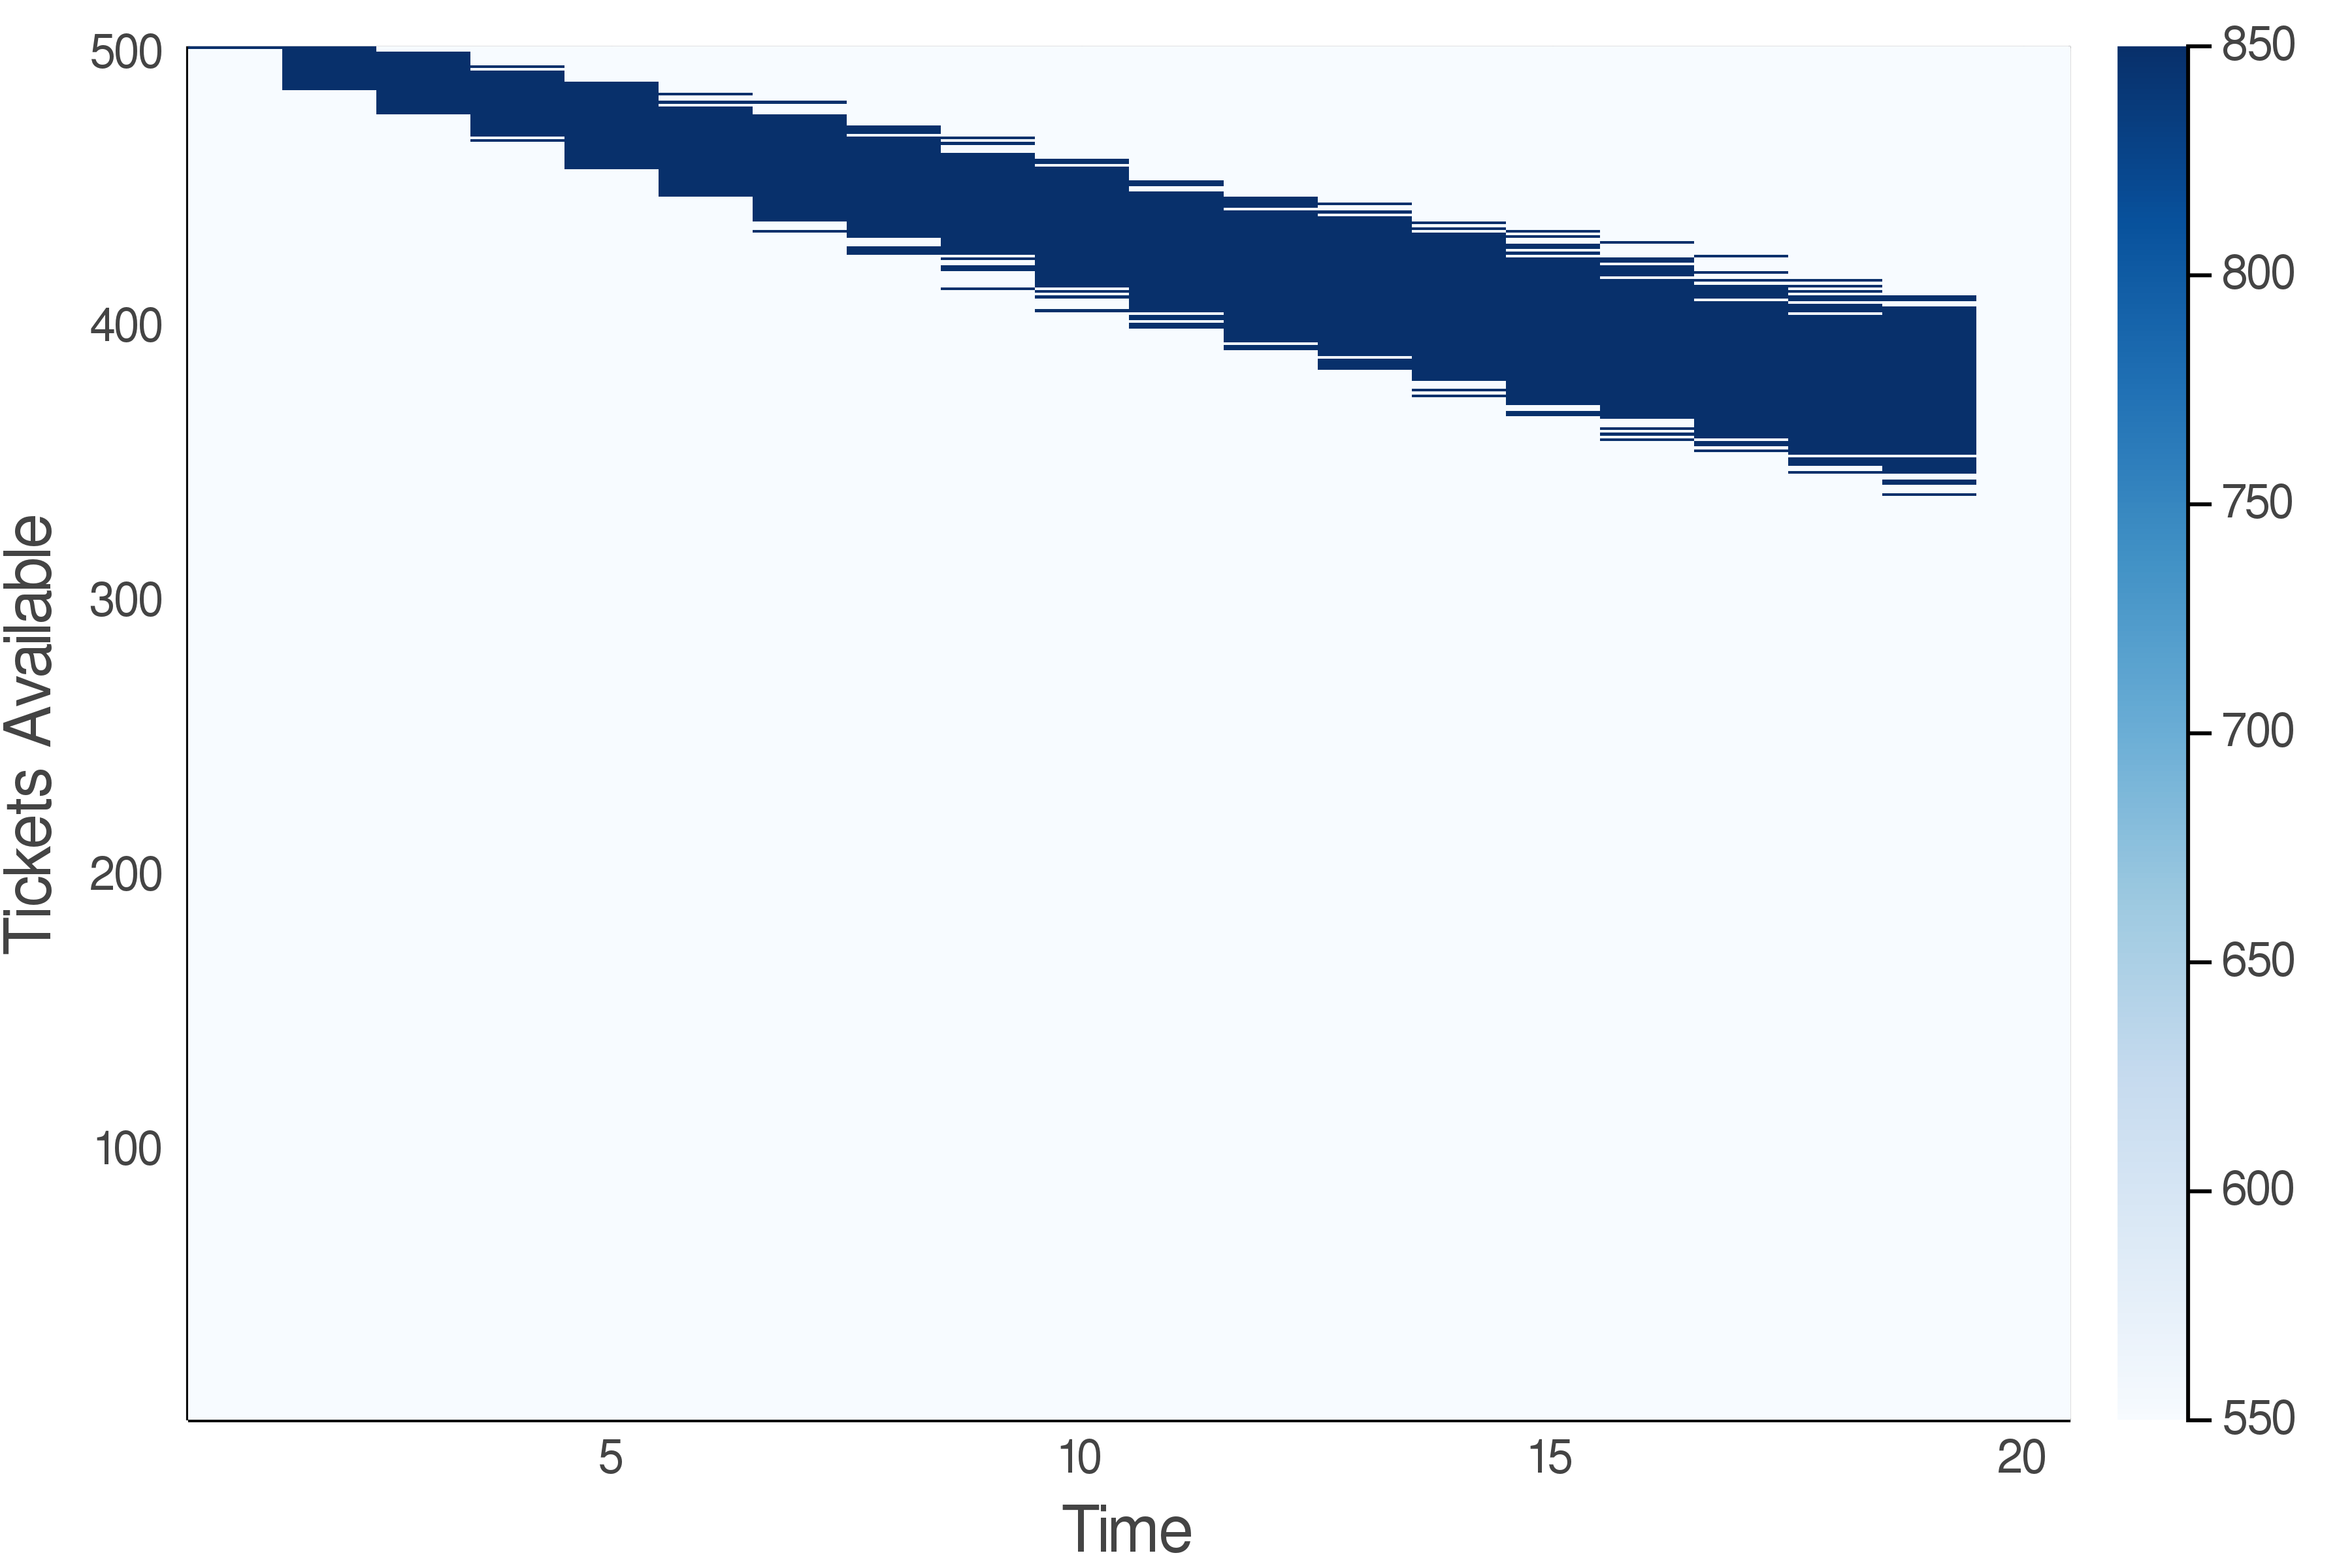
\includegraphics[width=0.3\linewidth]{final-paper/plots/doubleAgentStaticHigh-1policy.png}
    \caption{Optimal policies learned for the first fare class in the two fare class case using the cheapest price (\textit{left}), a random policy (\textit{center}), and the most expensive price (\textit{right}).}
\end{figure}

\begin{figure}[h!]
    \centering
    \label{fig:two-class-baselines-policy2}
    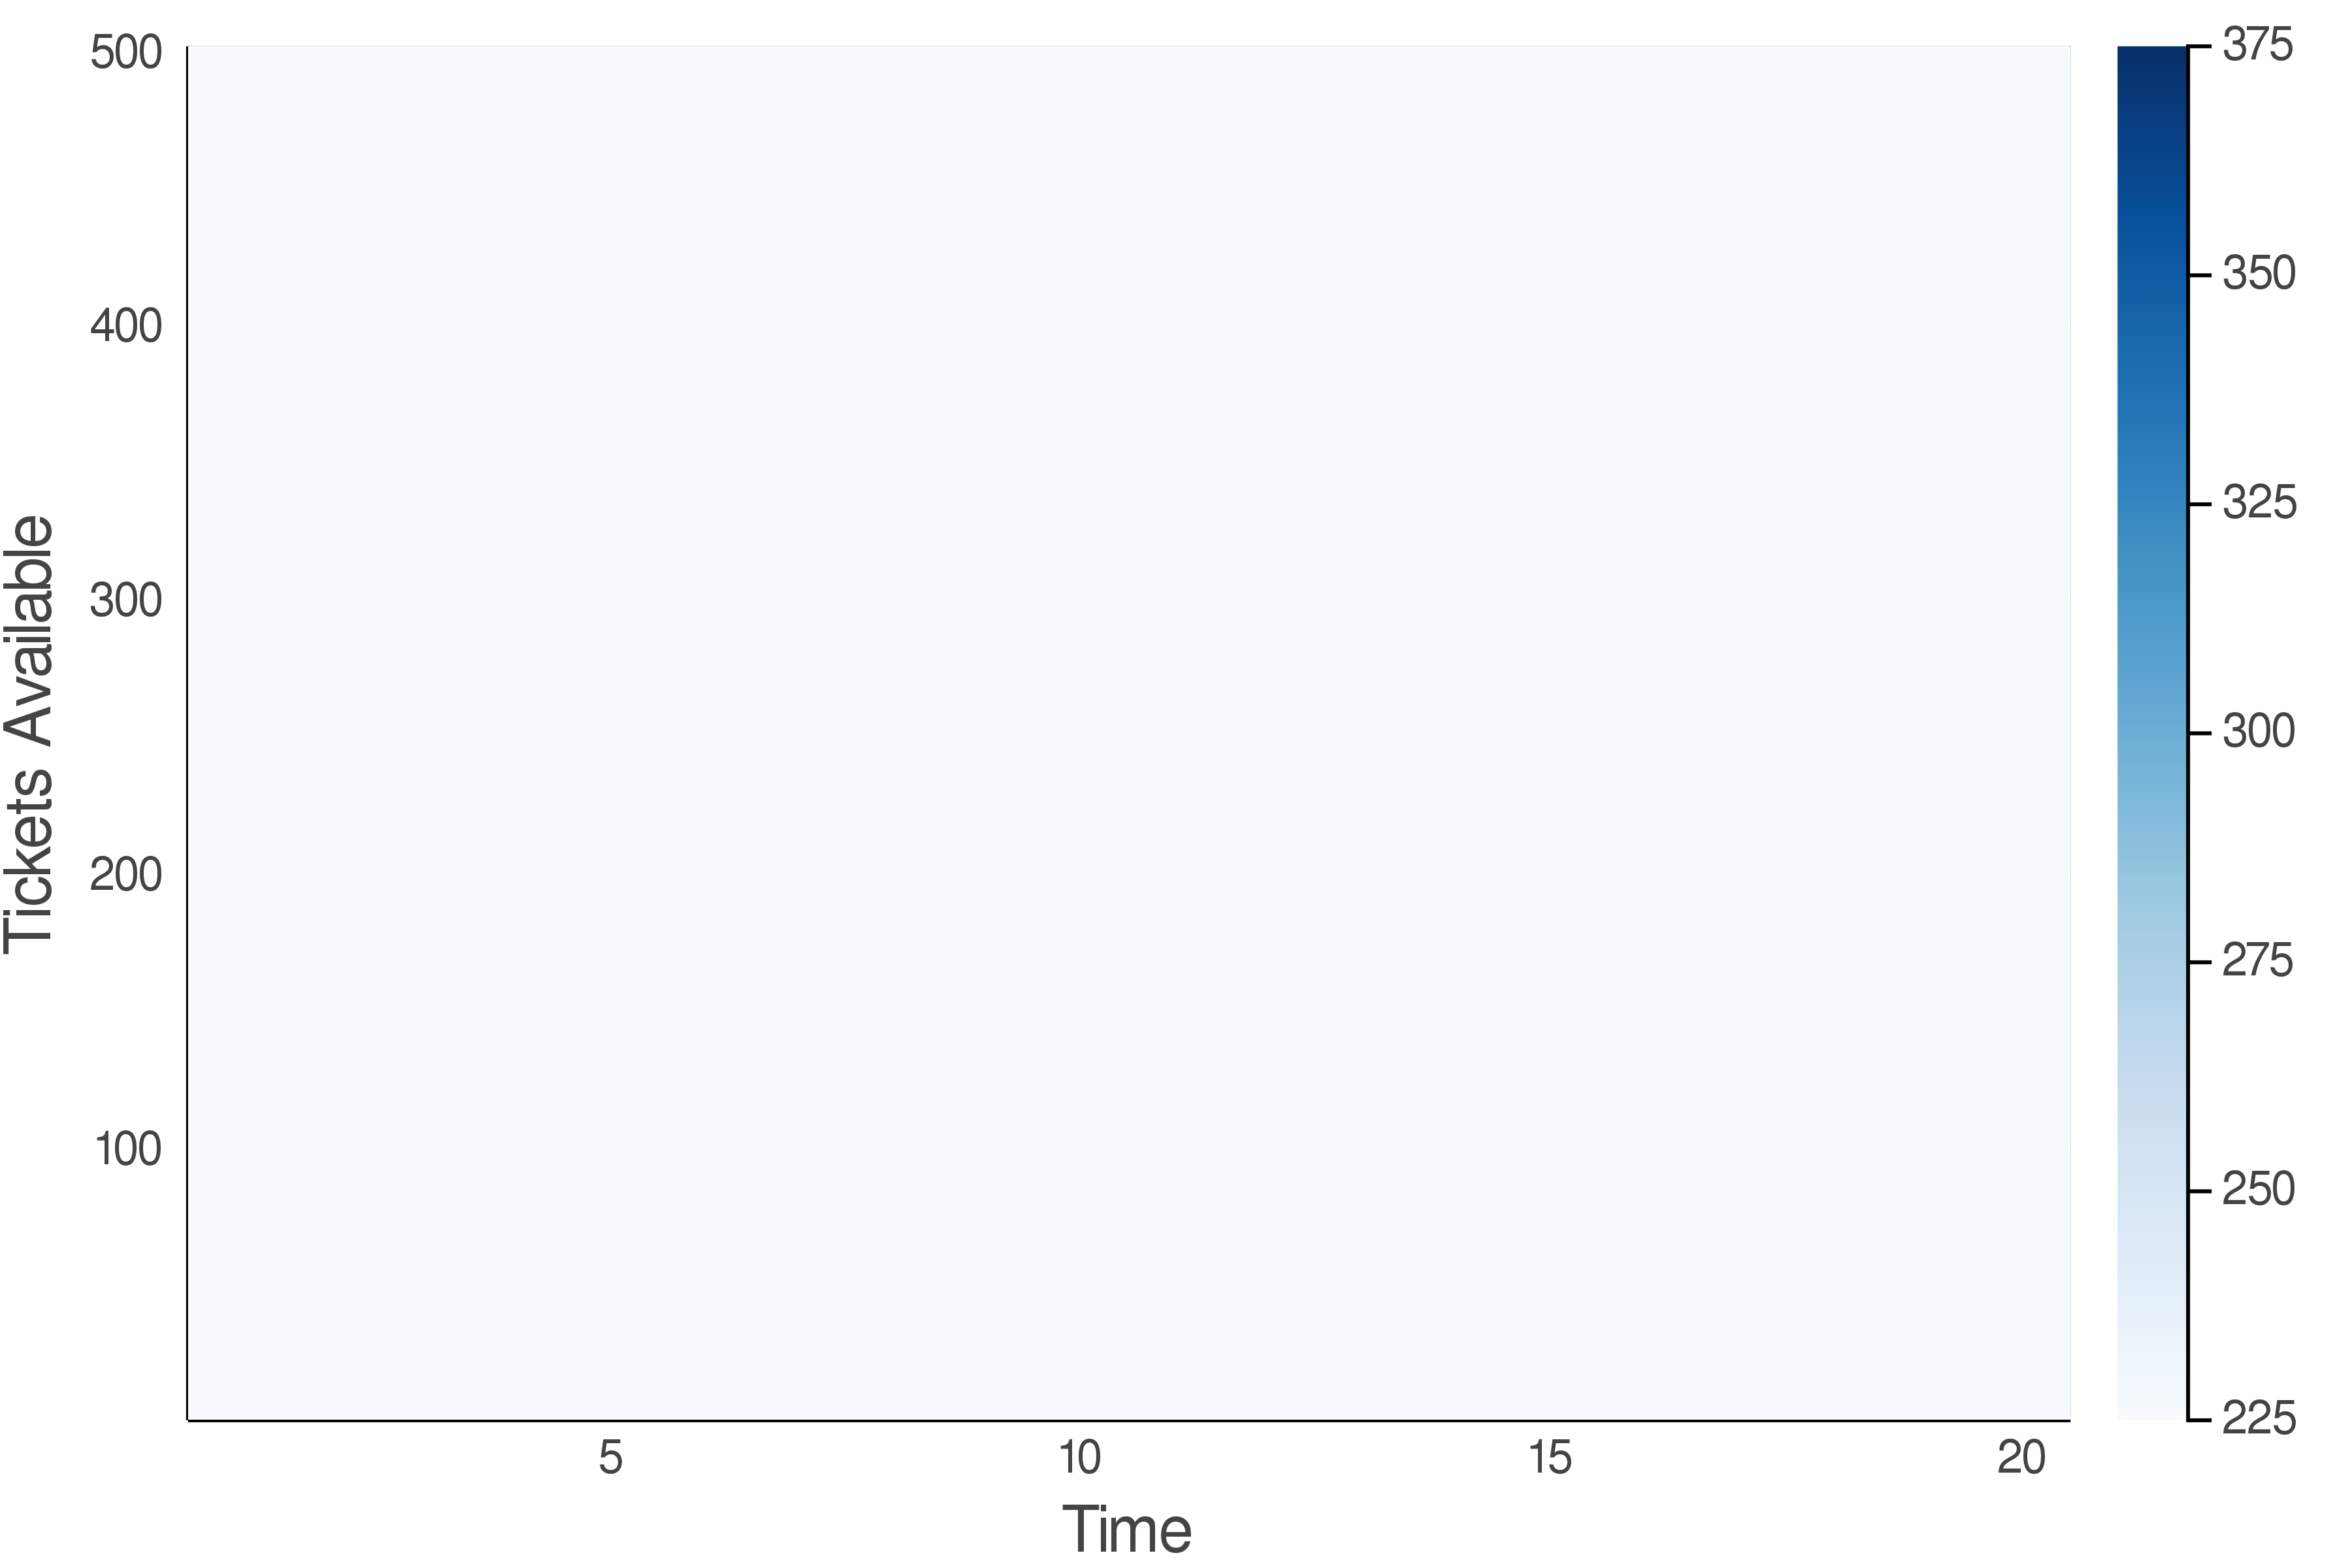
\includegraphics[width=0.3\linewidth]{final-paper/plots/doubleAgentStaticLow-2policy.png} \;
    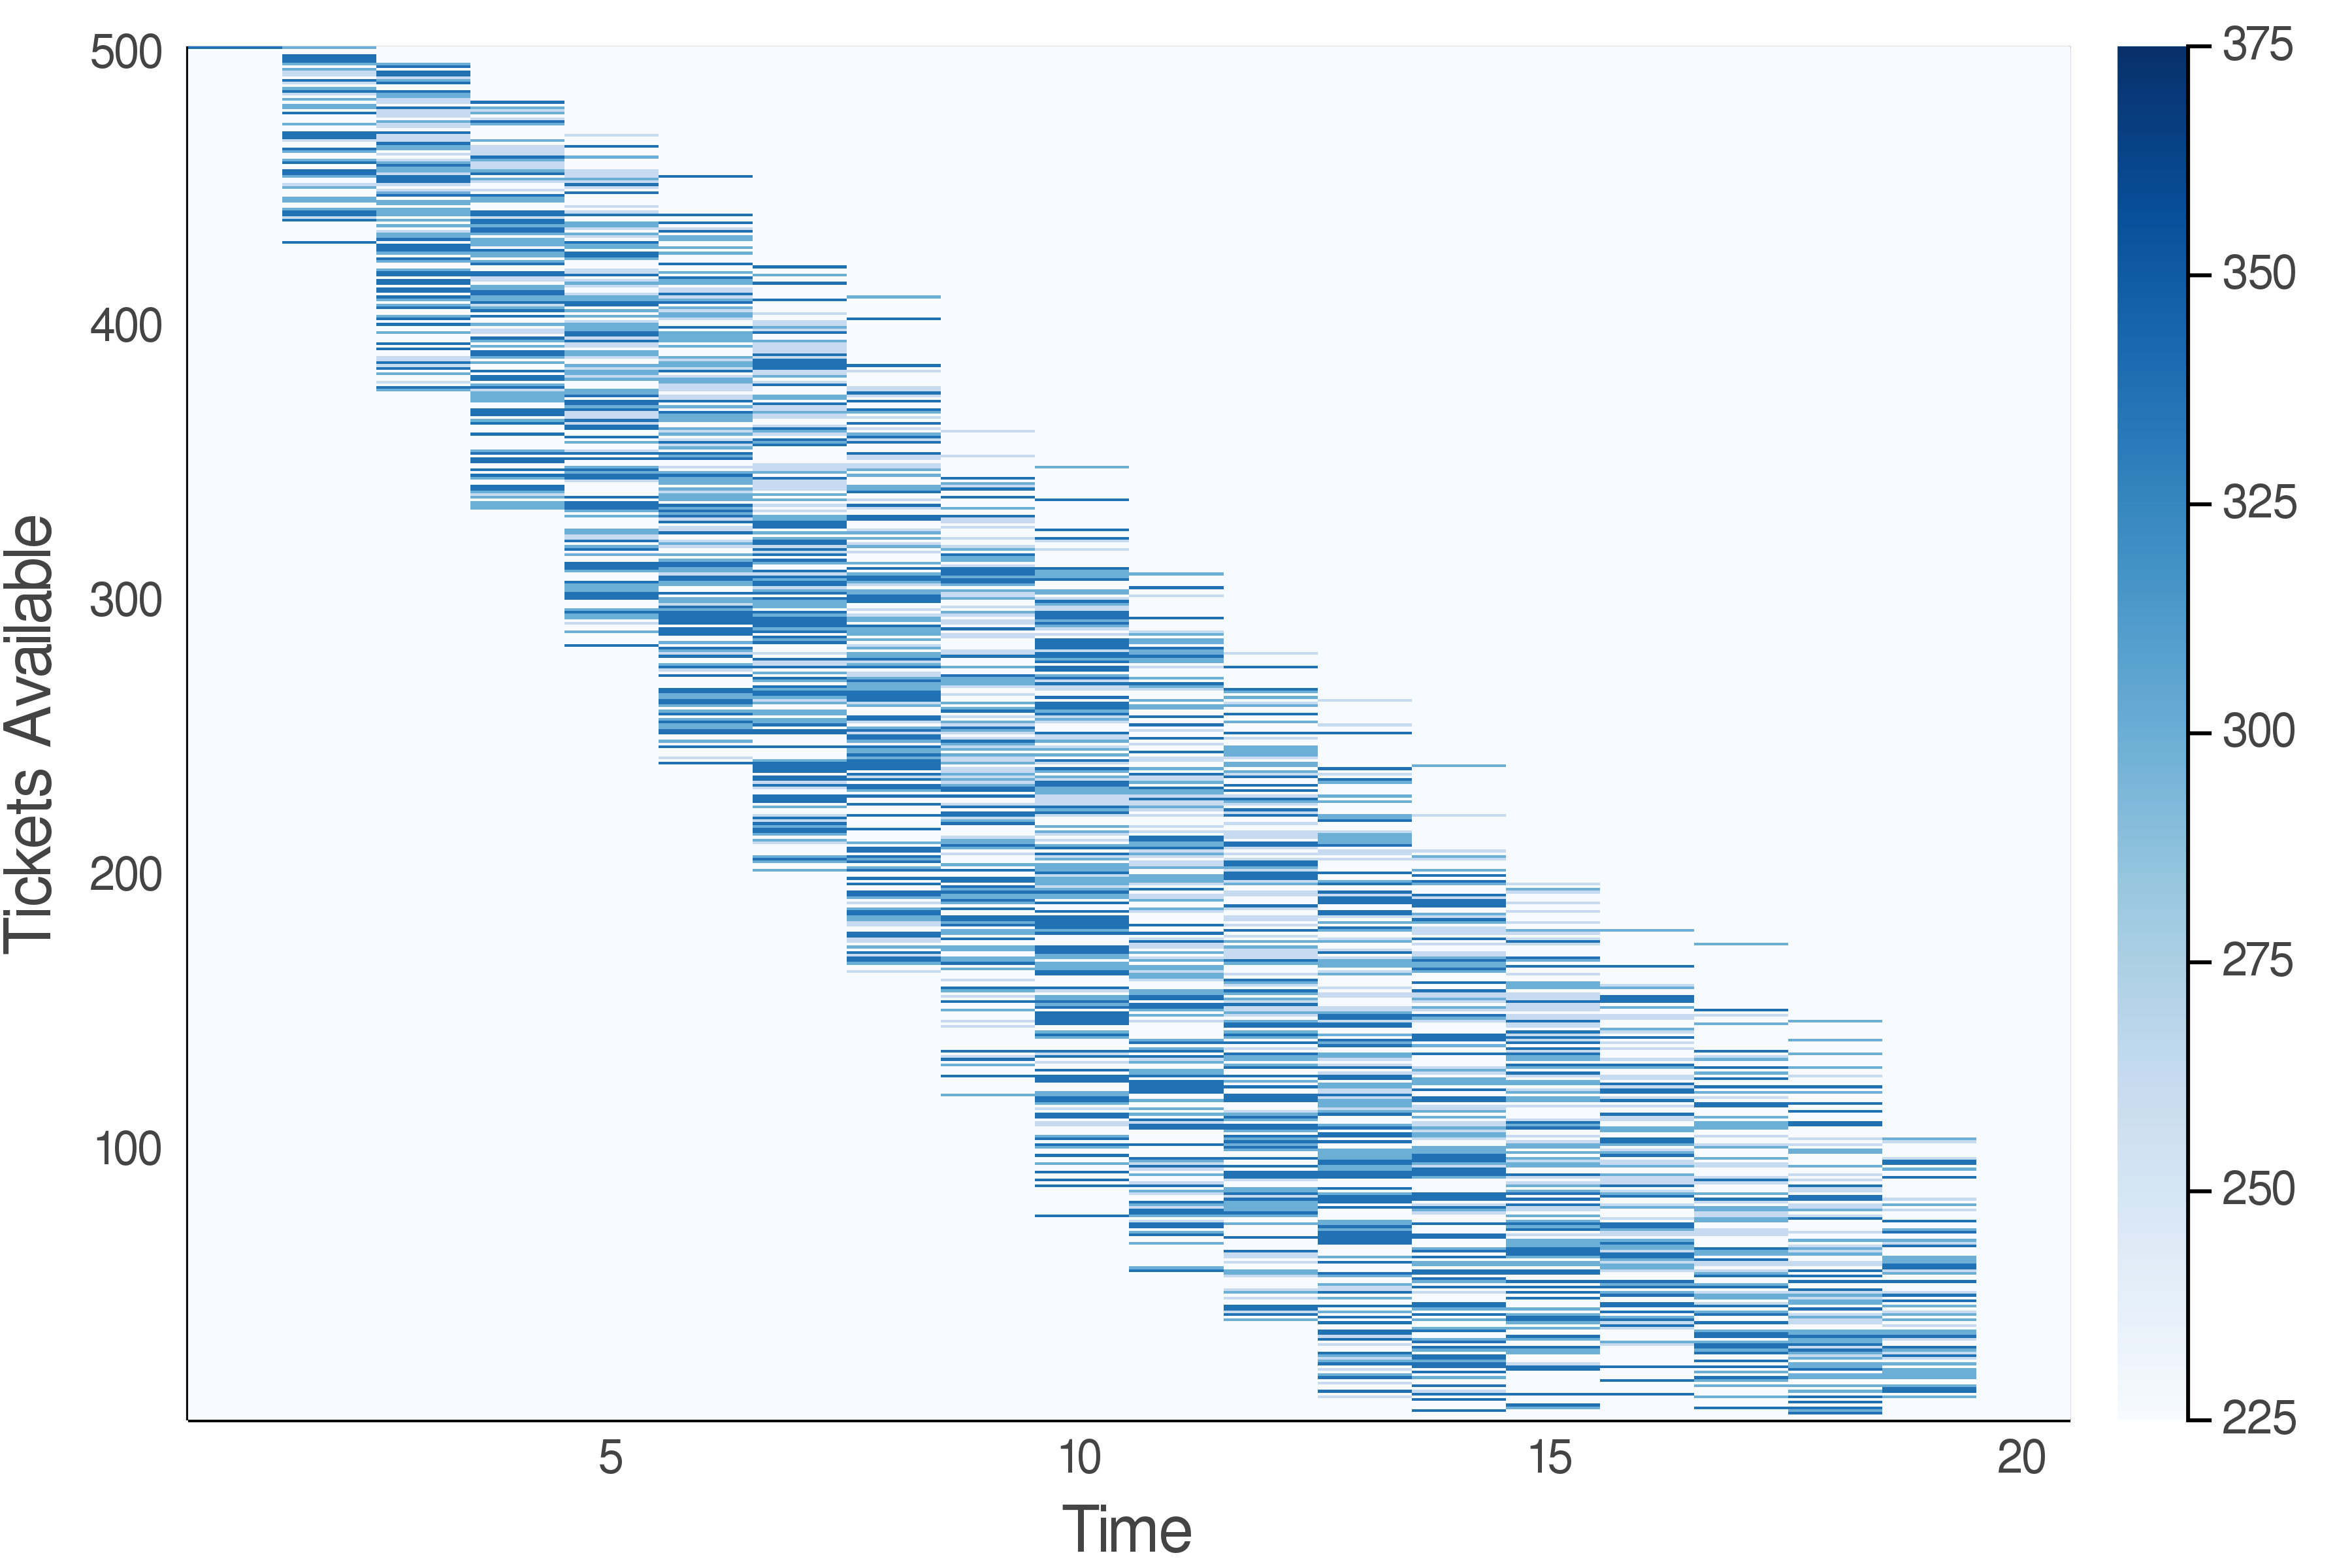
\includegraphics[width=0.3\linewidth]{final-paper/plots/doubleAgentRandom-2policy.png} \;
    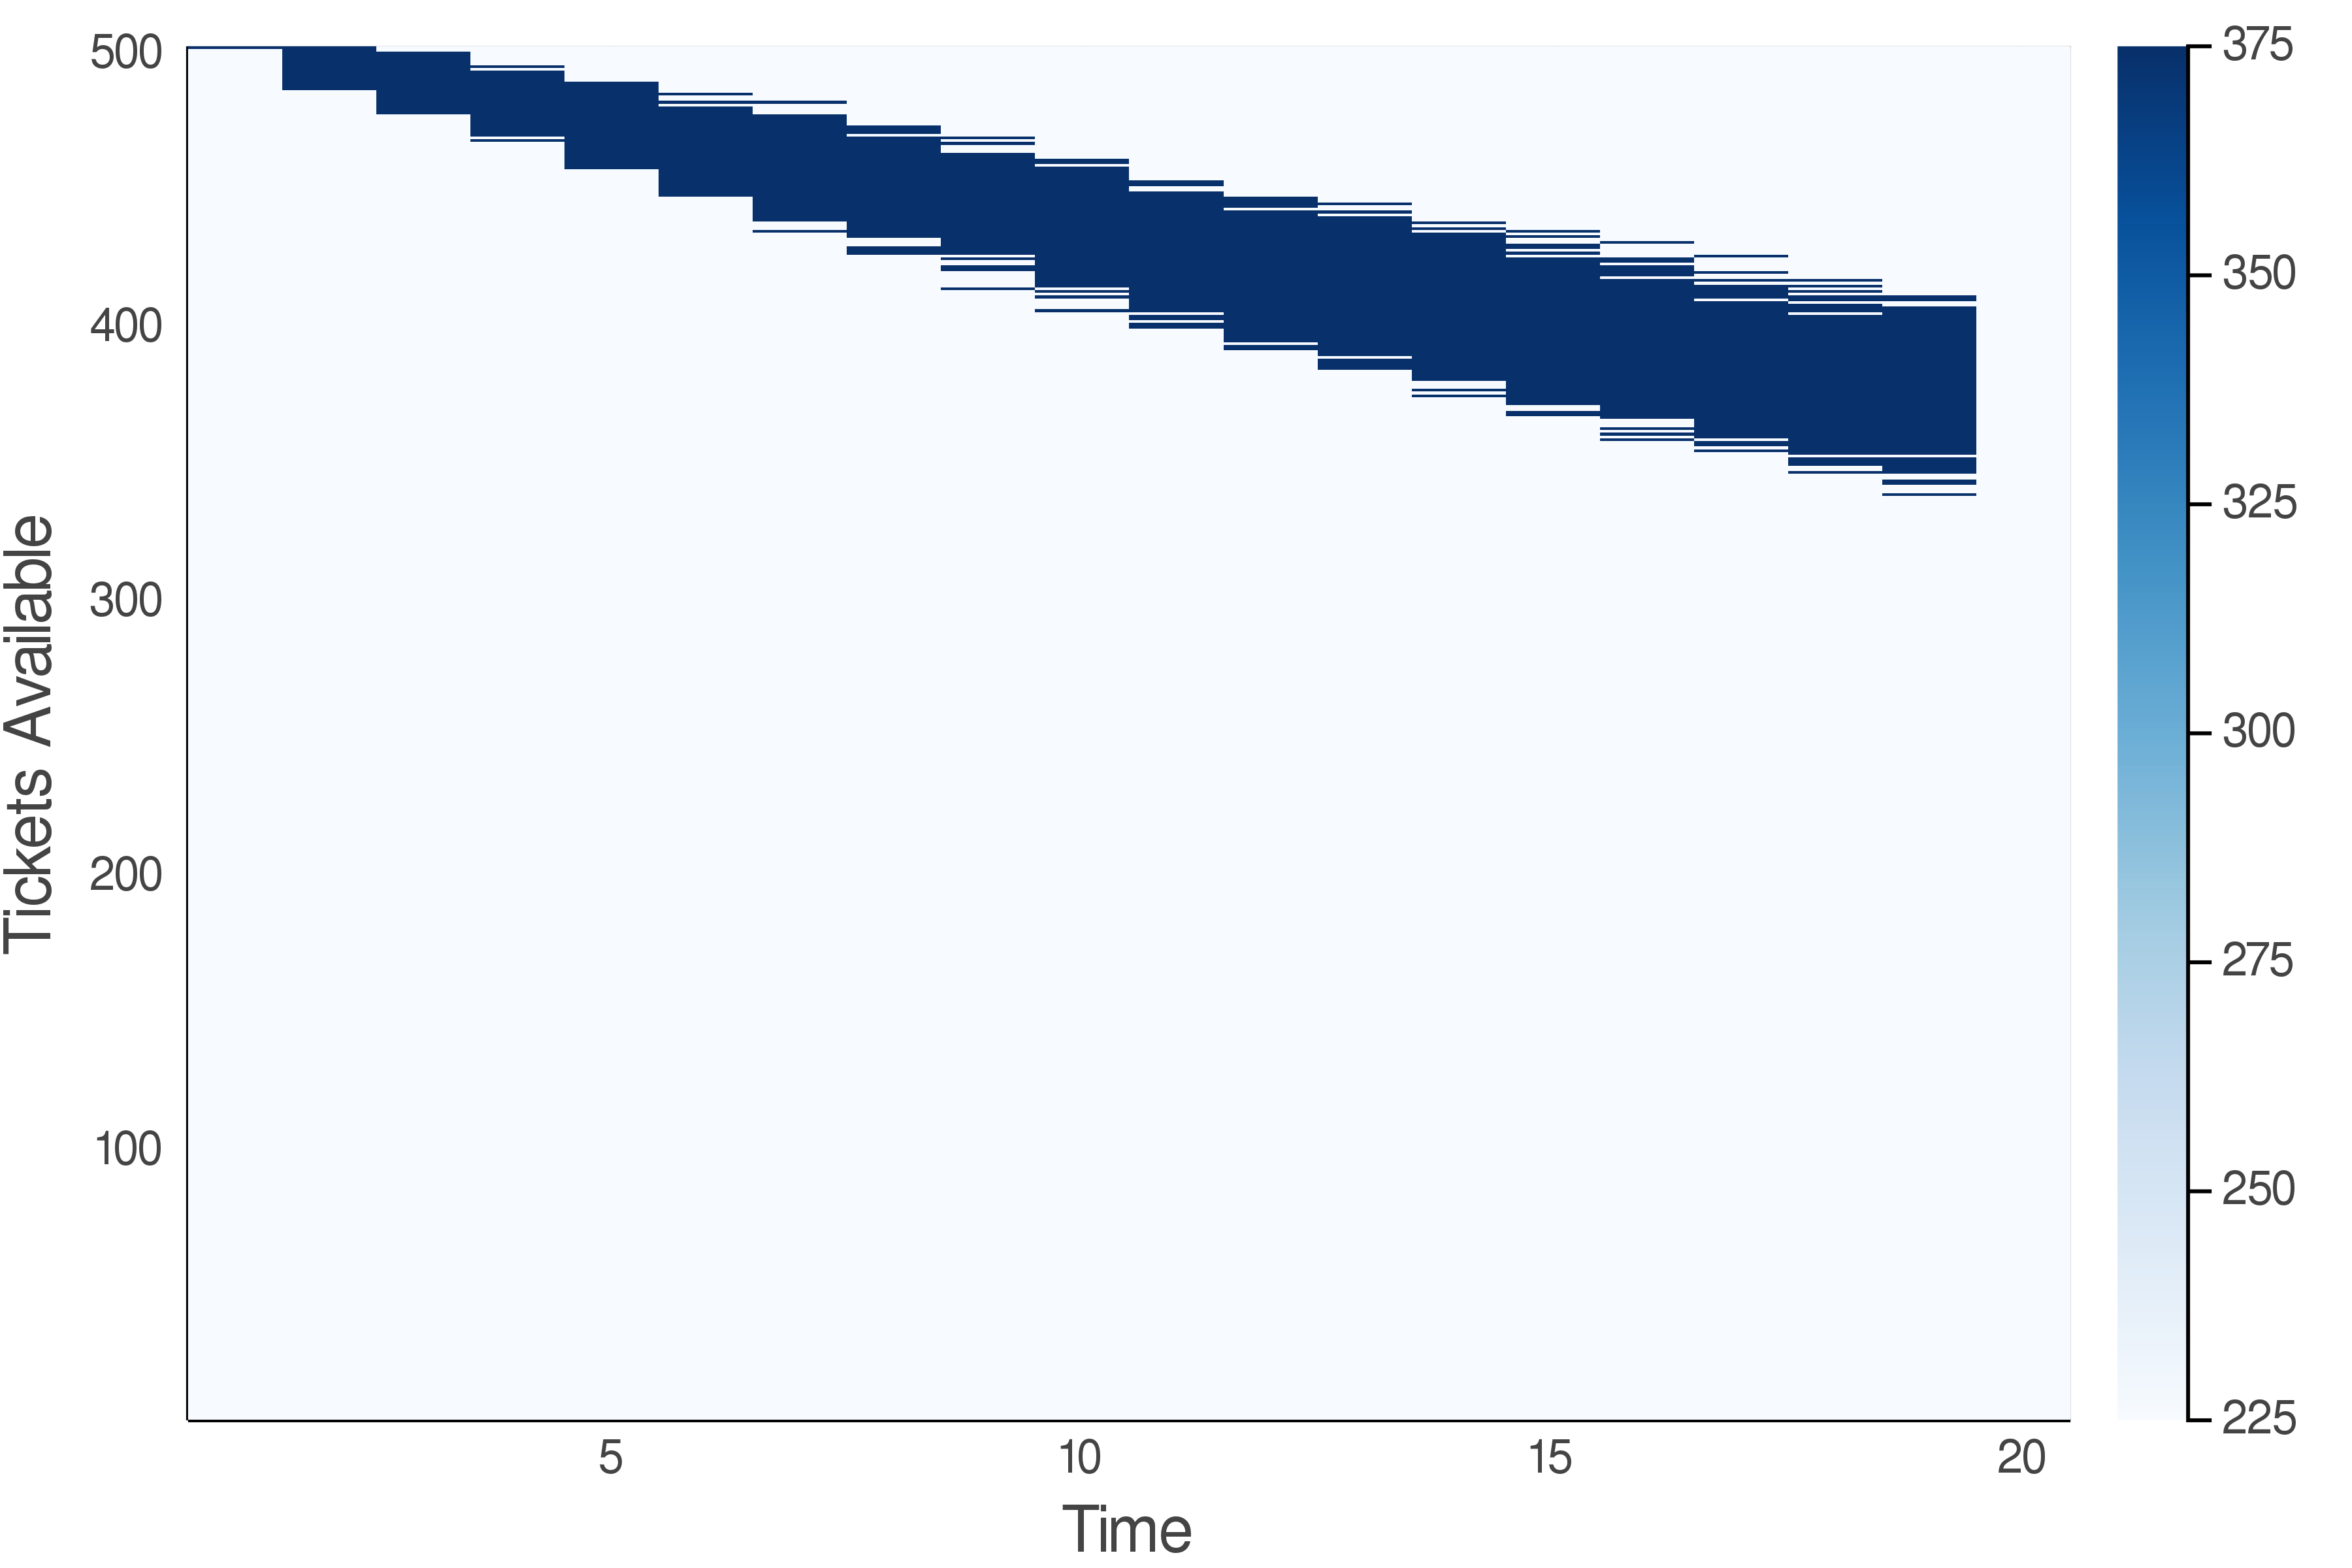
\includegraphics[width=0.3\linewidth]{final-paper/plots/doubleAgentStaticHigh-2policy.png}
    \caption{Optimal policies learned for the second fare class in the two fare class case using the cheapest price (\textit{left}), a random policy (\textit{center}), and the most expensive price (\textit{right}).}
\end{figure}

\clearpage

\section{Conclusion}

We introduced a factored multi-agent Markov decision process (MMDP) as a decision-theoretic approach to solving a multi-fare dynamic pricing problem and utilized model-free reinforcement learning algorithms to determine an approximately optimal policy for a specified set of fare classes. We demonstrated improvement over static and random default policies for a single-agent case and demonstrated improvement over static and random default policies in only some cases due to limited training time.

Further work could involve modifications to both the customer dynamics and learning frameworks. For example, the mean of the customers' willingness-to-pay threshold could be modeled to increase with time. Also, more complex learning frameworks could be used such as deep Q-learning (DQN) to globally approximate the state-action value function and thus improve generalization of the joint policy. The assumption that an agent can only set prices in a small, discrete set of prices is not poor in a general sense, however real agents can set prices in a continuous space (or at least at a fine resolution, e.g. \$1), so modifications could be made to the problem to enable a tractable solution for a fine-resolution discrete action set or continuous action space. Another modification could be to implement learning rate and epsilon-greedy annealing to stabilize the learning process and make to computation more efficient.

Additionally, the problem could be framed as a decentralized Markov decision process (DEC-MDP), where agents cannot communicate for free and the joint state is only jointly fully-observable, or the problem could be framed as a decentralized partially-observable Markov decision process (DEC-POMDP), where the individual state is partially-observable. These frameworks can improve the generalization of the joint policy to a wider variety of scenarios.

\section{Contributions}

Ross and Jonathan shared the workload for most aspects of the project. Ross worked more on developing the theoretical framework for the problem and Jonathan worked more on implementing the algorithms for solving the problem, but meetings were held regularly to discuss updates to the proposed approach, implementation of algorithms, generation of results and conclusion, and synthesis of the paper.

\bibliographystyle{aaai}
\bibliography{final}

\end{document}